%*************************************************************************
% A Classic Thesis Style
% An Homage to The Elements of Typographic Style
%
% Copyright (C) 2017 André Miede and Ivo Pletikosić
%
% If you like the style then I would appreciate a postcard. My address
% can be found in the file ClassicThesis.pdf. A collection of the
% postcards I received so far is available online at
% http://postcards.miede.de
%
% License:
% This program is free software; you can redistribute it and/or modify
% it under the terms of the GNU General Public License as published by
% the Free Software Foundation; either version 2 of the License, or
% (at your option) any later version.
%
% This program is distributed in the hope that it will be useful,
% but WITHOUT ANY WARRANTY; without even the implied warranty of
% MERCHANTABILITY or FITNESS FOR A PARTICULAR PURPOSE.  See the
% GNU General Public License for more details.
%
% You should have received a copy of the GNU General Public License
% along with this program; see the file COPYING.  If not, write to
% the Free Software Foundation, Inc., 59 Temple Place - Suite 330,
% Boston, MA 02111-1307, USA.
%
% PLEASE SEE ALSO THE AUTHORS' NOTE REGARDING THIS LICENSE
% IN THE DOCUMENTATION (ClassicThesis.pdf --> Chapter 1 / Chapter01.tex)
%*************************************************************************
\RequirePackage{silence} % :-\
    \WarningFilter{scrreprt}{Usage of package `titlesec'}
    %\WarningFilter{scrreprt}{Activating an ugly workaround}
    \WarningFilter{titlesec}{Non standard sectioning command detected}
\documentclass[ openright,titlepage,numbers=noenddot,headinclude,%twoside, %1headlines,% letterpaper a4paper
                footinclude=true,cleardoublepage=empty,abstractoff, % <--- obsolete, remove (todo)
                BCOR=5mm,paper=a4,fontsize=11pt,%11pt,a4paper,%
                ngerman,american,%lockflag%
                ]{scrreprt}

%*************************************************************************
% Note: Make all your adjustments in here
%*************************************************************************
% ****************************************************************************************************
% hdathesis-config.tex 
% Use it at the beginning of your thesis.tex, or as a LaTeX Preamble 
% in your thesis.{tex,lyx} with % ****************************************************************************************************
% hdathesis-config.tex 
% Use it at the beginning of your thesis.tex, or as a LaTeX Preamble 
% in your thesis.{tex,lyx} with % ****************************************************************************************************
% hdathesis-config.tex 
% Use it at the beginning of your thesis.tex, or as a LaTeX Preamble 
% in your thesis.{tex,lyx} with \input{hdathesis-config}
% ****************************************************************************************************

% ****************************************************************************************************
% 1. Personal data and user ad-hoc commands
% ****************************************************************************************************
\newcommand{\myTitle}{A Classic Thesis Style\xspace}
%\newcommand{\mySubtitle}{An Homage to The Elements of Typographic Style\xspace}
\newcommand{\myDegree}{Bachelor of Science (B.Sc.)\xspace} 
%\newcommand{\myDegree}{Bachelor of Arts (B.A.)\xspace}
%\newcommand{\myDegree}{Master of Science (M.Sc.)\xspace}
%\newcommand{\myDegree}{Master of Arts (M.A.)\xspace}
\newcommand{\myName}{Andr\'e Miede\xspace}
\newcommand{\myId}{081542\xspace}
\newcommand{\myProf}{Prof. Dr.-Ing. Michael Bredel\xspace}
\newcommand{\myOtherProf}{Prof. Dr. Martin Stiemerling\xspace}
\newcommand{\myFaculty}{Fachbereich Informatik\xspace}
\newcommand{\myUni}{Hochschule Darmstadt\xspace}
\newcommand{\myLocation}{Darmstadt\xspace}
\newcommand{\myTime}{20. Februar 2015\xspace}
\newcommand{\myVersion}{version 4.4\xspace}

% ****************************************************************************************************
% 2. Is it a master thesis?
% ****************************************************************************************************
%\PassOptionsToPackage{master}{hdahesis} % uncomment if this is a master thesis 

% ****************************************************************************************************
% 3. Does the thesis have a lock flag?
% ****************************************************************************************************
%\PassOptionsToPackage{lockflag}{hdathesis} % uncomment if this thesis has a lock flag 

% ****************************************************************************************************
% 4. Loading some handy packages
% ****************************************************************************************************
% ****************************************************************************************************
% Packages with options that might require adjustments
% ****************************************************************************************************

%\PassOptionsToPackage{ngerman,american}{babel}   % change this to your language(s)
% Spanish languages need extra options in order to work with this template
%\PassOptionsToPackage{spanish,es-lcroman}{babel}
\usepackage{babel}


% ****************************************************************************************************

% ****************************************************************************************************
% 1. Personal data and user ad-hoc commands
% ****************************************************************************************************
\newcommand{\myTitle}{A Classic Thesis Style\xspace}
%\newcommand{\mySubtitle}{An Homage to The Elements of Typographic Style\xspace}
\newcommand{\myDegree}{Bachelor of Science (B.Sc.)\xspace} 
%\newcommand{\myDegree}{Bachelor of Arts (B.A.)\xspace}
%\newcommand{\myDegree}{Master of Science (M.Sc.)\xspace}
%\newcommand{\myDegree}{Master of Arts (M.A.)\xspace}
\newcommand{\myName}{Andr\'e Miede\xspace}
\newcommand{\myId}{081542\xspace}
\newcommand{\myProf}{Prof. Dr.-Ing. Michael Bredel\xspace}
\newcommand{\myOtherProf}{Prof. Dr. Martin Stiemerling\xspace}
\newcommand{\myFaculty}{Fachbereich Informatik\xspace}
\newcommand{\myUni}{Hochschule Darmstadt\xspace}
\newcommand{\myLocation}{Darmstadt\xspace}
\newcommand{\myTime}{20. Februar 2015\xspace}
\newcommand{\myVersion}{version 4.4\xspace}

% ****************************************************************************************************
% 2. Is it a master thesis?
% ****************************************************************************************************
%\PassOptionsToPackage{master}{hdahesis} % uncomment if this is a master thesis 

% ****************************************************************************************************
% 3. Does the thesis have a lock flag?
% ****************************************************************************************************
%\PassOptionsToPackage{lockflag}{hdathesis} % uncomment if this thesis has a lock flag 

% ****************************************************************************************************
% 4. Loading some handy packages
% ****************************************************************************************************
% ****************************************************************************************************
% Packages with options that might require adjustments
% ****************************************************************************************************

%\PassOptionsToPackage{ngerman,american}{babel}   % change this to your language(s)
% Spanish languages need extra options in order to work with this template
%\PassOptionsToPackage{spanish,es-lcroman}{babel}
\usepackage{babel}


% ****************************************************************************************************

% ****************************************************************************************************
% 1. Personal data and user ad-hoc commands
% ****************************************************************************************************
\newcommand{\myTitle}{A Classic Thesis Style\xspace}
%\newcommand{\mySubtitle}{An Homage to The Elements of Typographic Style\xspace}
\newcommand{\myDegree}{Bachelor of Science (B.Sc.)\xspace} 
%\newcommand{\myDegree}{Bachelor of Arts (B.A.)\xspace}
%\newcommand{\myDegree}{Master of Science (M.Sc.)\xspace}
%\newcommand{\myDegree}{Master of Arts (M.A.)\xspace}
\newcommand{\myName}{Andr\'e Miede\xspace}
\newcommand{\myId}{081542\xspace}
\newcommand{\myProf}{Prof. Dr.-Ing. Michael Bredel\xspace}
\newcommand{\myOtherProf}{Prof. Dr. Martin Stiemerling\xspace}
\newcommand{\myFaculty}{Fachbereich Informatik\xspace}
\newcommand{\myUni}{Hochschule Darmstadt\xspace}
\newcommand{\myLocation}{Darmstadt\xspace}
\newcommand{\myTime}{20. Februar 2015\xspace}
\newcommand{\myVersion}{version 4.4\xspace}

% ****************************************************************************************************
% 2. Is it a master thesis?
% ****************************************************************************************************
%\PassOptionsToPackage{master}{hdahesis} % uncomment if this is a master thesis 

% ****************************************************************************************************
% 3. Does the thesis have a lock flag?
% ****************************************************************************************************
%\PassOptionsToPackage{lockflag}{hdathesis} % uncomment if this thesis has a lock flag 

% ****************************************************************************************************
% 4. Loading some handy packages
% ****************************************************************************************************
% ****************************************************************************************************
% Packages with options that might require adjustments
% ****************************************************************************************************

%\PassOptionsToPackage{ngerman,american}{babel}   % change this to your language(s)
% Spanish languages need extra options in order to work with this template
%\PassOptionsToPackage{spanish,es-lcroman}{babel}
\usepackage{babel}


% ****************************************************************************************************
% classicthesis-config.tex
% formerly known as loadpackages.sty, classicthesis-ldpkg.sty, and classicthesis-preamble.sty
% Use it at the beginning of your ClassicThesis.tex, or as a LaTeX Preamble
% in your ClassicThesis.{tex,lyx} with % ****************************************************************************************************
% classicthesis-config.tex
% formerly known as loadpackages.sty, classicthesis-ldpkg.sty, and classicthesis-preamble.sty
% Use it at the beginning of your ClassicThesis.tex, or as a LaTeX Preamble
% in your ClassicThesis.{tex,lyx} with % ****************************************************************************************************
% classicthesis-config.tex
% formerly known as loadpackages.sty, classicthesis-ldpkg.sty, and classicthesis-preamble.sty
% Use it at the beginning of your ClassicThesis.tex, or as a LaTeX Preamble
% in your ClassicThesis.{tex,lyx} with \input{classicthesis-config}
% ****************************************************************************************************
% If you like the classicthesis, then I would appreciate a postcard.
% My address can be found in the file ClassicThesis.pdf. A collection
% of the postcards I received so far is available online at
% http://postcards.miede.de
% ****************************************************************************************************


% ****************************************************************************************************
% 0. Set the encoding of your files. UTF-8 is the only sensible encoding nowadays. If you can't read
% äöüßáéçèê∂åëæƒÏ€ then change the encoding setting in your editor, not the line below. If your editor
% does not support utf8 use another editor!
% ****************************************************************************************************
\PassOptionsToPackage{utf8}{inputenc}
  \usepackage{inputenc}

% ****************************************************************************************************
% 1. Configure classicthesis for your needs here, e.g., remove "drafting" below
% in order to deactivate the time-stamp on the pages
% (see ClassicThesis.pdf for more information):
% ****************************************************************************************************
\PassOptionsToPackage{
  drafting=false,   % print version information on the bottom of the pages
  tocaligned=false, % the left column of the toc will be aligned (no indentation)
  dottedtoc=true,   % page numbers in ToC flushed right
  parts=true,       % use part division
  eulerchapternumbers=true, % use AMS Euler for chapter font (otherwise Palatino)
  linedheaders=false,       % chaper headers will have line above and beneath
  floatperchapter=true,     % numbering per chapter for all floats (i.e., Figure 1.1)
  listings=true,    % load listings package and setup LoL
  subfig=true,      % setup for preloaded subfig package
  eulermath=false,  % use awesome Euler fonts for mathematical formulae (only with pdfLaTeX)
  beramono=true,    % toggle a nice monospaced font (w/ bold)
  minionpro=false   % setup for minion pro font; use minion pro small caps as well (only with pdfLaTeX)
}{classicthesis}


% ****************************************************************************************************
% 2. Personal data and user ad-hoc commands
% ****************************************************************************************************
%\newcommand{\myTitle}{A Classic Thesis Style\xspace}
%\newcommand{\mySubtitle}{An Homage to The Elements of Typographic Style\xspace}
%\newcommand{\myDegree}{Doktor-Ingenieur (Dr.-Ing.)\xspace}
%\newcommand{\myName}{André Miede\xspace}
%\newcommand{\myProf}{Put name here\xspace}
%\newcommand{\myOtherProf}{Put name here\xspace}
%\newcommand{\mySupervisor}{Put name here\xspace}
%\newcommand{\myFaculty}{Put data here\xspace}
%\newcommand{\myDepartment}{Put data here\xspace}
%\newcommand{\myUni}{Put data here\xspace}
%\newcommand{\myLocation}{Saarbrücken\xspace}
%\newcommand{\myTime}{October 2017\xspace}
%\newcommand{\myVersion}{version 4.4}

% ********************************************************************
% Setup, finetuning, and useful commands
% ********************************************************************
\newcounter{dummy} % necessary for correct hyperlinks (to index, bib, etc.)
\newlength{\abcd} % for ab..z string length calculation
\providecommand{\mLyX}{L\kern-.1667em\lower.25em\hbox{Y}\kern-.125emX\@}
\newcommand{\ie}{i.\,e.}
\newcommand{\Ie}{I.\,e.}
\newcommand{\eg}{e.\,g.}
\newcommand{\Eg}{E.\,g.}
% ****************************************************************************************************


% ****************************************************************************************************
% 3. Loading some handy packages
% ****************************************************************************************************
% ********************************************************************
% Packages with options that might require adjustments
% ********************************************************************
%\PassOptionsToPackage{ngerman,american}{babel}   % change this to your language(s), main language last
% Spanish languages need extra options in order to work with this template
%\PassOptionsToPackage{spanish,es-lcroman}{babel}
\usepackage{babel}

\usepackage{csquotes}

\PassOptionsToPackage{%
  %backend=biber,bibencoding=utf8, %instead of bibtex
  backend=bibtex8,bibencoding=ascii,%
  language=auto,%
  style=numeric-comp,%
  %style=alphabetic,%
  %style=authoryear-comp, % Author 1999, 2010
  %bibstyle=authoryear,dashed=false, % dashed: substitute rep. author with ---
  sorting=nyt, % name, year, title
  maxbibnames=10, % default: 3, et al.
  %backref=true,%
  natbib=true % natbib compatibility mode (\citep and \citet still work)
}{biblatex}
  \usepackage{biblatex}

\PassOptionsToPackage{fleqn}{amsmath}       % math environments and more by the AMS
  \usepackage{amsmath}

\PassOptionsToPackage{doublespacing}{hdathesis}  % options: abbrev exam big wiwi english master
  \usepackage{hdathesis}

% ********************************************************************
% General useful packages
% ********************************************************************
\PassOptionsToPackage{T1}{fontenc} % T2A for cyrillics
  \usepackage{fontenc}
\usepackage{textcomp} % fix warning with missing font shapes
\usepackage{scrhack} % fix warnings when using KOMA with listings package
\usepackage{xspace} % to get the spacing after macros right
\usepackage{mparhack} % get marginpar right
%\usepackage{fixltx2e} % fixes some LaTeX stuff --> since 2015 in the LaTeX kernel (see below)
% \usepackage[latest]{latexrelease} % emulate newer kernel version if older is detected
\PassOptionsToPackage{printonlyused,smaller}{acronym}
  \usepackage{acronym} % nice macros for handling all acronyms in the thesis
  %\renewcommand{\bflabel}[1]{{#1}\hfill} % fix the list of acronyms --> no longer working
  %\renewcommand*{\acsfont}[1]{\textsc{#1}}
  %\renewcommand*{\aclabelfont}[1]{\acsfont{#1}}
  %\def\bflabel#1{{#1\hfill}}
  \def\bflabel#1{{\acsfont{#1}\hfill}}
  \def\aclabelfont#1{\acsfont{#1}}
% ****************************************************************************************************
%\usepackage{pgfplots} % External TikZ/PGF support (thanks to Andreas Nautsch)
%\usetikzlibrary{external}
%\tikzexternalize[mode=list and make, prefix=ext-tikz/]
% ****************************************************************************************************


% ****************************************************************************************************
% 4. Setup floats: tables, (sub)figures, and captions
% ****************************************************************************************************
\usepackage{tabularx} % better tables
  \setlength{\extrarowheight}{3pt} % increase table row height
\newcommand{\tableheadline}[1]{\multicolumn{1}{c}{\spacedlowsmallcaps{#1}}}
\newcommand{\myfloatalign}{\centering} % to be used with each float for alignment
\usepackage{caption}
% Thanks to cgnieder and Claus Lahiri
% http://tex.stackexchange.com/questions/69349/spacedlowsmallcaps-in-caption-label
% [REMOVED DUE TO OTHER PROBLEMS, SEE ISSUE #82]
%\DeclareCaptionLabelFormat{smallcaps}{\bothIfFirst{#1}{~}\MakeTextLowercase{\textsc{#2}}}
%\captionsetup{font=small,labelformat=smallcaps} % format=hang,
\captionsetup{font=small} % format=hang,
\usepackage{subfig}
% ****************************************************************************************************


% ****************************************************************************************************
% 5. Setup code listings
% ****************************************************************************************************
\usepackage{listings}
%\lstset{emph={trueIndex,root},emphstyle=\color{BlueViolet}}%\underbar} % for special keywords
\lstset{language=[LaTeX]Tex,%C++,
  morekeywords={PassOptionsToPackage,selectlanguage},
  keywordstyle=\color{RoyalBlue},%\bfseries,
  basicstyle=\small\ttfamily,
  %identifierstyle=\color{NavyBlue},
  commentstyle=\color{Green}\ttfamily,
  stringstyle=\rmfamily,
  numbers=none,%left,%
  numberstyle=\scriptsize,%\tiny
  stepnumber=5,
  numbersep=8pt,
  showstringspaces=false,
  breaklines=true,
  %frameround=ftff,
  %frame=single,
  belowcaptionskip=.75\baselineskip
  %frame=L
}
% ****************************************************************************************************


% ****************************************************************************************************
% 6. PDFLaTeX, hyperreferences, and citation backreferences
% ****************************************************************************************************
% ********************************************************************
% Using PDFLaTeX
% ********************************************************************
\PassOptionsToPackage{hyperfootnotes=false,pdfpagelabels}{hyperref}
  \usepackage{hyperref}  % backref linktocpage pagebackref
%\ifpdf
%\pdfcompresslevel=9
%\pdfadjustspacing=1
%\fi
%\PassOptionsToPackage{pdftex}{graphicx} %%%IVO: driver will be chosen automatically
  \usepackage{graphicx}


% ********************************************************************
% Hyperreferences
% ********************************************************************
\hypersetup{%
  %draft, % hyperref's draft mode, for printing see below
  colorlinks=true, linktocpage=true, pdfstartpage=3, pdfstartview=FitV,%
  % uncomment the following line if you want to have black links (e.g., for printing)
  %colorlinks=false, linktocpage=false, pdfstartpage=3, pdfstartview=FitV, pdfborder={0 0 0},%
  breaklinks=true, pdfpagemode=UseNone, pageanchor=true, pdfpagemode=UseOutlines,%
  plainpages=false, bookmarksnumbered, bookmarksopen=true, bookmarksopenlevel=1,%
  hypertexnames=true, pdfhighlight=/O,%nesting=true,%frenchlinks,%
  urlcolor=webbrown, linkcolor=RoyalBlue, citecolor=webgreen, %pagecolor=RoyalBlue,%
  %urlcolor=Black, linkcolor=Black, citecolor=Black, %pagecolor=Black,%
  pdftitle={\myTitle},%
  pdfauthor={\textcopyright\ \myName, \myUni, \myFaculty},%
  pdfsubject={},%
  pdfkeywords={},%
  pdfcreator={pdfLaTeX},%
  pdfproducer={LaTeX with hyperref and classicthesis}%
}

% ********************************************************************
% Setup autoreferences
% ********************************************************************
% There are some issues regarding autorefnames
% http://www.ureader.de/msg/136221647.aspx
% http://www.tex.ac.uk/cgi-bin/texfaq2html?label=latexwords
% you have to redefine the makros for the
% language you use, e.g., american, ngerman
% (as chosen when loading babel/AtBeginDocument)
% ********************************************************************
\makeatletter
\@ifpackageloaded{babel}%
  {%
    \addto\extrasamerican{%
      \renewcommand*{\figureautorefname}{Figure}%
      \renewcommand*{\tableautorefname}{Table}%
      \renewcommand*{\partautorefname}{Part}%
      \renewcommand*{\chapterautorefname}{Chapter}%
      \renewcommand*{\sectionautorefname}{Section}%
      \renewcommand*{\subsectionautorefname}{Section}%
      \renewcommand*{\subsubsectionautorefname}{Section}%
    }%
    \addto\extrasngerman{%
      \renewcommand*{\paragraphautorefname}{Absatz}%
      \renewcommand*{\subparagraphautorefname}{Unterabsatz}%
      \renewcommand*{\footnoteautorefname}{Fu\"snote}%
      \renewcommand*{\FancyVerbLineautorefname}{Zeile}%
      \renewcommand*{\theoremautorefname}{Theorem}%
      \renewcommand*{\appendixautorefname}{Anhang}%
      \renewcommand*{\equationautorefname}{Gleichung}%
      \renewcommand*{\itemautorefname}{Punkt}%
    }%
      % Fix to getting autorefs for subfigures right (thanks to Belinda Vogt for changing the definition)
      \providecommand{\subfigureautorefname}{\figureautorefname}%
    }{\relax}
\makeatother


% ****************************************************************************************************
% 7. Last calls before the bar closes
% ****************************************************************************************************
% ********************************************************************
% Development Stuff
% ********************************************************************
\listfiles
%\PassOptionsToPackage{l2tabu,orthodox,abort}{nag}
%  \usepackage{nag}
%\PassOptionsToPackage{warning, all}{onlyamsmath}
%  \usepackage{onlyamsmath}

% ********************************************************************
% Last, but not least...
% ********************************************************************
\usepackage{classicthesis}
% ****************************************************************************************************


% ****************************************************************************************************
% 8. Further adjustments (experimental)
% ****************************************************************************************************
% ********************************************************************
% Changing the text area
% ********************************************************************
%\areaset[current]{312pt}{761pt} % 686 (factor 2.2) + 33 head + 42 head \the\footskip
%\setlength{\marginparwidth}{7em}%
%\setlength{\marginparsep}{2em}%

% ********************************************************************
% Using different fonts
% ********************************************************************
%\usepackage[oldstylenums]{kpfonts} % oldstyle notextcomp
%\usepackage[osf]{libertine}
%\usepackage[light,condensed,math]{iwona}
%\renewcommand{\sfdefault}{iwona}
%\usepackage{lmodern} % <-- no osf support :-(
%\usepackage{cfr-lm} %
%\usepackage[urw-garamond]{mathdesign} <-- no osf support :-(
%\usepackage[default,osfigures]{opensans} % scale=0.95
%\usepackage[sfdefault]{FiraSans}
% ********************************************************************
% \usepackage[largesc,osf]{newpxtext}
% Used to fix these:
% https://bitbucket.org/amiede/classicthesis/issues/139/italics-in-pallatino-capitals-chapter
% https://bitbucket.org/amiede/classicthesis/issues/45/problema-testatine-su-classicthesis-style
% ********************************************************************
%\linespread{1.05} % a bit more for Palatino
% ****************************************************************************************************

% ****************************************************************************************************
% If you like the classicthesis, then I would appreciate a postcard.
% My address can be found in the file ClassicThesis.pdf. A collection
% of the postcards I received so far is available online at
% http://postcards.miede.de
% ****************************************************************************************************


% ****************************************************************************************************
% 0. Set the encoding of your files. UTF-8 is the only sensible encoding nowadays. If you can't read
% äöüßáéçèê∂åëæƒÏ€ then change the encoding setting in your editor, not the line below. If your editor
% does not support utf8 use another editor!
% ****************************************************************************************************
\PassOptionsToPackage{utf8}{inputenc}
  \usepackage{inputenc}

% ****************************************************************************************************
% 1. Configure classicthesis for your needs here, e.g., remove "drafting" below
% in order to deactivate the time-stamp on the pages
% (see ClassicThesis.pdf for more information):
% ****************************************************************************************************
\PassOptionsToPackage{
  drafting=false,   % print version information on the bottom of the pages
  tocaligned=false, % the left column of the toc will be aligned (no indentation)
  dottedtoc=true,   % page numbers in ToC flushed right
  parts=true,       % use part division
  eulerchapternumbers=true, % use AMS Euler for chapter font (otherwise Palatino)
  linedheaders=false,       % chaper headers will have line above and beneath
  floatperchapter=true,     % numbering per chapter for all floats (i.e., Figure 1.1)
  listings=true,    % load listings package and setup LoL
  subfig=true,      % setup for preloaded subfig package
  eulermath=false,  % use awesome Euler fonts for mathematical formulae (only with pdfLaTeX)
  beramono=true,    % toggle a nice monospaced font (w/ bold)
  minionpro=false   % setup for minion pro font; use minion pro small caps as well (only with pdfLaTeX)
}{classicthesis}


% ****************************************************************************************************
% 2. Personal data and user ad-hoc commands
% ****************************************************************************************************
%\newcommand{\myTitle}{A Classic Thesis Style\xspace}
%\newcommand{\mySubtitle}{An Homage to The Elements of Typographic Style\xspace}
%\newcommand{\myDegree}{Doktor-Ingenieur (Dr.-Ing.)\xspace}
%\newcommand{\myName}{André Miede\xspace}
%\newcommand{\myProf}{Put name here\xspace}
%\newcommand{\myOtherProf}{Put name here\xspace}
%\newcommand{\mySupervisor}{Put name here\xspace}
%\newcommand{\myFaculty}{Put data here\xspace}
%\newcommand{\myDepartment}{Put data here\xspace}
%\newcommand{\myUni}{Put data here\xspace}
%\newcommand{\myLocation}{Saarbrücken\xspace}
%\newcommand{\myTime}{October 2017\xspace}
%\newcommand{\myVersion}{version 4.4}

% ********************************************************************
% Setup, finetuning, and useful commands
% ********************************************************************
\newcounter{dummy} % necessary for correct hyperlinks (to index, bib, etc.)
\newlength{\abcd} % for ab..z string length calculation
\providecommand{\mLyX}{L\kern-.1667em\lower.25em\hbox{Y}\kern-.125emX\@}
\newcommand{\ie}{i.\,e.}
\newcommand{\Ie}{I.\,e.}
\newcommand{\eg}{e.\,g.}
\newcommand{\Eg}{E.\,g.}
% ****************************************************************************************************


% ****************************************************************************************************
% 3. Loading some handy packages
% ****************************************************************************************************
% ********************************************************************
% Packages with options that might require adjustments
% ********************************************************************
%\PassOptionsToPackage{ngerman,american}{babel}   % change this to your language(s), main language last
% Spanish languages need extra options in order to work with this template
%\PassOptionsToPackage{spanish,es-lcroman}{babel}
\usepackage{babel}

\usepackage{csquotes}

\PassOptionsToPackage{%
  %backend=biber,bibencoding=utf8, %instead of bibtex
  backend=bibtex8,bibencoding=ascii,%
  language=auto,%
  style=numeric-comp,%
  %style=alphabetic,%
  %style=authoryear-comp, % Author 1999, 2010
  %bibstyle=authoryear,dashed=false, % dashed: substitute rep. author with ---
  sorting=nyt, % name, year, title
  maxbibnames=10, % default: 3, et al.
  %backref=true,%
  natbib=true % natbib compatibility mode (\citep and \citet still work)
}{biblatex}
  \usepackage{biblatex}

\PassOptionsToPackage{fleqn}{amsmath}       % math environments and more by the AMS
  \usepackage{amsmath}

\PassOptionsToPackage{doublespacing}{hdathesis}  % options: abbrev exam big wiwi english master
  \usepackage{hdathesis}

% ********************************************************************
% General useful packages
% ********************************************************************
\PassOptionsToPackage{T1}{fontenc} % T2A for cyrillics
  \usepackage{fontenc}
\usepackage{textcomp} % fix warning with missing font shapes
\usepackage{scrhack} % fix warnings when using KOMA with listings package
\usepackage{xspace} % to get the spacing after macros right
\usepackage{mparhack} % get marginpar right
%\usepackage{fixltx2e} % fixes some LaTeX stuff --> since 2015 in the LaTeX kernel (see below)
% \usepackage[latest]{latexrelease} % emulate newer kernel version if older is detected
\PassOptionsToPackage{printonlyused,smaller}{acronym}
  \usepackage{acronym} % nice macros for handling all acronyms in the thesis
  %\renewcommand{\bflabel}[1]{{#1}\hfill} % fix the list of acronyms --> no longer working
  %\renewcommand*{\acsfont}[1]{\textsc{#1}}
  %\renewcommand*{\aclabelfont}[1]{\acsfont{#1}}
  %\def\bflabel#1{{#1\hfill}}
  \def\bflabel#1{{\acsfont{#1}\hfill}}
  \def\aclabelfont#1{\acsfont{#1}}
% ****************************************************************************************************
%\usepackage{pgfplots} % External TikZ/PGF support (thanks to Andreas Nautsch)
%\usetikzlibrary{external}
%\tikzexternalize[mode=list and make, prefix=ext-tikz/]
% ****************************************************************************************************


% ****************************************************************************************************
% 4. Setup floats: tables, (sub)figures, and captions
% ****************************************************************************************************
\usepackage{tabularx} % better tables
  \setlength{\extrarowheight}{3pt} % increase table row height
\newcommand{\tableheadline}[1]{\multicolumn{1}{c}{\spacedlowsmallcaps{#1}}}
\newcommand{\myfloatalign}{\centering} % to be used with each float for alignment
\usepackage{caption}
% Thanks to cgnieder and Claus Lahiri
% http://tex.stackexchange.com/questions/69349/spacedlowsmallcaps-in-caption-label
% [REMOVED DUE TO OTHER PROBLEMS, SEE ISSUE #82]
%\DeclareCaptionLabelFormat{smallcaps}{\bothIfFirst{#1}{~}\MakeTextLowercase{\textsc{#2}}}
%\captionsetup{font=small,labelformat=smallcaps} % format=hang,
\captionsetup{font=small} % format=hang,
\usepackage{subfig}
% ****************************************************************************************************


% ****************************************************************************************************
% 5. Setup code listings
% ****************************************************************************************************
\usepackage{listings}
%\lstset{emph={trueIndex,root},emphstyle=\color{BlueViolet}}%\underbar} % for special keywords
\lstset{language=[LaTeX]Tex,%C++,
  morekeywords={PassOptionsToPackage,selectlanguage},
  keywordstyle=\color{RoyalBlue},%\bfseries,
  basicstyle=\small\ttfamily,
  %identifierstyle=\color{NavyBlue},
  commentstyle=\color{Green}\ttfamily,
  stringstyle=\rmfamily,
  numbers=none,%left,%
  numberstyle=\scriptsize,%\tiny
  stepnumber=5,
  numbersep=8pt,
  showstringspaces=false,
  breaklines=true,
  %frameround=ftff,
  %frame=single,
  belowcaptionskip=.75\baselineskip
  %frame=L
}
% ****************************************************************************************************


% ****************************************************************************************************
% 6. PDFLaTeX, hyperreferences, and citation backreferences
% ****************************************************************************************************
% ********************************************************************
% Using PDFLaTeX
% ********************************************************************
\PassOptionsToPackage{hyperfootnotes=false,pdfpagelabels}{hyperref}
  \usepackage{hyperref}  % backref linktocpage pagebackref
%\ifpdf
%\pdfcompresslevel=9
%\pdfadjustspacing=1
%\fi
%\PassOptionsToPackage{pdftex}{graphicx} %%%IVO: driver will be chosen automatically
  \usepackage{graphicx}


% ********************************************************************
% Hyperreferences
% ********************************************************************
\hypersetup{%
  %draft, % hyperref's draft mode, for printing see below
  colorlinks=true, linktocpage=true, pdfstartpage=3, pdfstartview=FitV,%
  % uncomment the following line if you want to have black links (e.g., for printing)
  %colorlinks=false, linktocpage=false, pdfstartpage=3, pdfstartview=FitV, pdfborder={0 0 0},%
  breaklinks=true, pdfpagemode=UseNone, pageanchor=true, pdfpagemode=UseOutlines,%
  plainpages=false, bookmarksnumbered, bookmarksopen=true, bookmarksopenlevel=1,%
  hypertexnames=true, pdfhighlight=/O,%nesting=true,%frenchlinks,%
  urlcolor=webbrown, linkcolor=RoyalBlue, citecolor=webgreen, %pagecolor=RoyalBlue,%
  %urlcolor=Black, linkcolor=Black, citecolor=Black, %pagecolor=Black,%
  pdftitle={\myTitle},%
  pdfauthor={\textcopyright\ \myName, \myUni, \myFaculty},%
  pdfsubject={},%
  pdfkeywords={},%
  pdfcreator={pdfLaTeX},%
  pdfproducer={LaTeX with hyperref and classicthesis}%
}

% ********************************************************************
% Setup autoreferences
% ********************************************************************
% There are some issues regarding autorefnames
% http://www.ureader.de/msg/136221647.aspx
% http://www.tex.ac.uk/cgi-bin/texfaq2html?label=latexwords
% you have to redefine the makros for the
% language you use, e.g., american, ngerman
% (as chosen when loading babel/AtBeginDocument)
% ********************************************************************
\makeatletter
\@ifpackageloaded{babel}%
  {%
    \addto\extrasamerican{%
      \renewcommand*{\figureautorefname}{Figure}%
      \renewcommand*{\tableautorefname}{Table}%
      \renewcommand*{\partautorefname}{Part}%
      \renewcommand*{\chapterautorefname}{Chapter}%
      \renewcommand*{\sectionautorefname}{Section}%
      \renewcommand*{\subsectionautorefname}{Section}%
      \renewcommand*{\subsubsectionautorefname}{Section}%
    }%
    \addto\extrasngerman{%
      \renewcommand*{\paragraphautorefname}{Absatz}%
      \renewcommand*{\subparagraphautorefname}{Unterabsatz}%
      \renewcommand*{\footnoteautorefname}{Fu\"snote}%
      \renewcommand*{\FancyVerbLineautorefname}{Zeile}%
      \renewcommand*{\theoremautorefname}{Theorem}%
      \renewcommand*{\appendixautorefname}{Anhang}%
      \renewcommand*{\equationautorefname}{Gleichung}%
      \renewcommand*{\itemautorefname}{Punkt}%
    }%
      % Fix to getting autorefs for subfigures right (thanks to Belinda Vogt for changing the definition)
      \providecommand{\subfigureautorefname}{\figureautorefname}%
    }{\relax}
\makeatother


% ****************************************************************************************************
% 7. Last calls before the bar closes
% ****************************************************************************************************
% ********************************************************************
% Development Stuff
% ********************************************************************
\listfiles
%\PassOptionsToPackage{l2tabu,orthodox,abort}{nag}
%  \usepackage{nag}
%\PassOptionsToPackage{warning, all}{onlyamsmath}
%  \usepackage{onlyamsmath}

% ********************************************************************
% Last, but not least...
% ********************************************************************
\usepackage{classicthesis}
% ****************************************************************************************************


% ****************************************************************************************************
% 8. Further adjustments (experimental)
% ****************************************************************************************************
% ********************************************************************
% Changing the text area
% ********************************************************************
%\areaset[current]{312pt}{761pt} % 686 (factor 2.2) + 33 head + 42 head \the\footskip
%\setlength{\marginparwidth}{7em}%
%\setlength{\marginparsep}{2em}%

% ********************************************************************
% Using different fonts
% ********************************************************************
%\usepackage[oldstylenums]{kpfonts} % oldstyle notextcomp
%\usepackage[osf]{libertine}
%\usepackage[light,condensed,math]{iwona}
%\renewcommand{\sfdefault}{iwona}
%\usepackage{lmodern} % <-- no osf support :-(
%\usepackage{cfr-lm} %
%\usepackage[urw-garamond]{mathdesign} <-- no osf support :-(
%\usepackage[default,osfigures]{opensans} % scale=0.95
%\usepackage[sfdefault]{FiraSans}
% ********************************************************************
% \usepackage[largesc,osf]{newpxtext}
% Used to fix these:
% https://bitbucket.org/amiede/classicthesis/issues/139/italics-in-pallatino-capitals-chapter
% https://bitbucket.org/amiede/classicthesis/issues/45/problema-testatine-su-classicthesis-style
% ********************************************************************
%\linespread{1.05} % a bit more for Palatino
% ****************************************************************************************************

% ****************************************************************************************************
% If you like the classicthesis, then I would appreciate a postcard.
% My address can be found in the file ClassicThesis.pdf. A collection
% of the postcards I received so far is available online at
% http://postcards.miede.de
% ****************************************************************************************************


% ****************************************************************************************************
% 0. Set the encoding of your files. UTF-8 is the only sensible encoding nowadays. If you can't read
% äöüßáéçèê∂åëæƒÏ€ then change the encoding setting in your editor, not the line below. If your editor
% does not support utf8 use another editor!
% ****************************************************************************************************
\PassOptionsToPackage{utf8}{inputenc}
  \usepackage{inputenc}

% ****************************************************************************************************
% 1. Configure classicthesis for your needs here, e.g., remove "drafting" below
% in order to deactivate the time-stamp on the pages
% (see ClassicThesis.pdf for more information):
% ****************************************************************************************************
\PassOptionsToPackage{
  drafting=false,   % print version information on the bottom of the pages
  tocaligned=false, % the left column of the toc will be aligned (no indentation)
  dottedtoc=true,   % page numbers in ToC flushed right
  parts=true,       % use part division
  eulerchapternumbers=true, % use AMS Euler for chapter font (otherwise Palatino)
  linedheaders=false,       % chaper headers will have line above and beneath
  floatperchapter=true,     % numbering per chapter for all floats (i.e., Figure 1.1)
  listings=true,    % load listings package and setup LoL
  subfig=true,      % setup for preloaded subfig package
  eulermath=false,  % use awesome Euler fonts for mathematical formulae (only with pdfLaTeX)
  beramono=true,    % toggle a nice monospaced font (w/ bold)
  minionpro=false   % setup for minion pro font; use minion pro small caps as well (only with pdfLaTeX)
}{classicthesis}


% ****************************************************************************************************
% 2. Personal data and user ad-hoc commands
% ****************************************************************************************************
%\newcommand{\myTitle}{A Classic Thesis Style\xspace}
%\newcommand{\mySubtitle}{An Homage to The Elements of Typographic Style\xspace}
%\newcommand{\myDegree}{Doktor-Ingenieur (Dr.-Ing.)\xspace}
%\newcommand{\myName}{André Miede\xspace}
%\newcommand{\myProf}{Put name here\xspace}
%\newcommand{\myOtherProf}{Put name here\xspace}
%\newcommand{\mySupervisor}{Put name here\xspace}
%\newcommand{\myFaculty}{Put data here\xspace}
%\newcommand{\myDepartment}{Put data here\xspace}
%\newcommand{\myUni}{Put data here\xspace}
%\newcommand{\myLocation}{Saarbrücken\xspace}
%\newcommand{\myTime}{October 2017\xspace}
%\newcommand{\myVersion}{version 4.4}

% ********************************************************************
% Setup, finetuning, and useful commands
% ********************************************************************
\newcounter{dummy} % necessary for correct hyperlinks (to index, bib, etc.)
\newlength{\abcd} % for ab..z string length calculation
\providecommand{\mLyX}{L\kern-.1667em\lower.25em\hbox{Y}\kern-.125emX\@}
\newcommand{\ie}{i.\,e.}
\newcommand{\Ie}{I.\,e.}
\newcommand{\eg}{e.\,g.}
\newcommand{\Eg}{E.\,g.}
% ****************************************************************************************************


% ****************************************************************************************************
% 3. Loading some handy packages
% ****************************************************************************************************
% ********************************************************************
% Packages with options that might require adjustments
% ********************************************************************
%\PassOptionsToPackage{ngerman,american}{babel}   % change this to your language(s), main language last
% Spanish languages need extra options in order to work with this template
%\PassOptionsToPackage{spanish,es-lcroman}{babel}
\usepackage{babel}

\usepackage{csquotes}

\PassOptionsToPackage{%
  %backend=biber,bibencoding=utf8, %instead of bibtex
  backend=bibtex8,bibencoding=ascii,%
  language=auto,%
  style=numeric-comp,%
  %style=alphabetic,%
  %style=authoryear-comp, % Author 1999, 2010
  %bibstyle=authoryear,dashed=false, % dashed: substitute rep. author with ---
  sorting=nyt, % name, year, title
  maxbibnames=10, % default: 3, et al.
  %backref=true,%
  natbib=true % natbib compatibility mode (\citep and \citet still work)
}{biblatex}
  \usepackage{biblatex}

\PassOptionsToPackage{fleqn}{amsmath}       % math environments and more by the AMS
  \usepackage{amsmath}

\PassOptionsToPackage{doublespacing}{hdathesis}  % options: abbrev exam big wiwi english master
  \usepackage{hdathesis}

% ********************************************************************
% General useful packages
% ********************************************************************
\PassOptionsToPackage{T1}{fontenc} % T2A for cyrillics
  \usepackage{fontenc}
\usepackage{textcomp} % fix warning with missing font shapes
\usepackage{scrhack} % fix warnings when using KOMA with listings package
\usepackage{xspace} % to get the spacing after macros right
\usepackage{mparhack} % get marginpar right
%\usepackage{fixltx2e} % fixes some LaTeX stuff --> since 2015 in the LaTeX kernel (see below)
% \usepackage[latest]{latexrelease} % emulate newer kernel version if older is detected
\PassOptionsToPackage{printonlyused,smaller}{acronym}
  \usepackage{acronym} % nice macros for handling all acronyms in the thesis
  %\renewcommand{\bflabel}[1]{{#1}\hfill} % fix the list of acronyms --> no longer working
  %\renewcommand*{\acsfont}[1]{\textsc{#1}}
  %\renewcommand*{\aclabelfont}[1]{\acsfont{#1}}
  %\def\bflabel#1{{#1\hfill}}
  \def\bflabel#1{{\acsfont{#1}\hfill}}
  \def\aclabelfont#1{\acsfont{#1}}
% ****************************************************************************************************
%\usepackage{pgfplots} % External TikZ/PGF support (thanks to Andreas Nautsch)
%\usetikzlibrary{external}
%\tikzexternalize[mode=list and make, prefix=ext-tikz/]
% ****************************************************************************************************


% ****************************************************************************************************
% 4. Setup floats: tables, (sub)figures, and captions
% ****************************************************************************************************
\usepackage{tabularx} % better tables
  \setlength{\extrarowheight}{3pt} % increase table row height
\newcommand{\tableheadline}[1]{\multicolumn{1}{c}{\spacedlowsmallcaps{#1}}}
\newcommand{\myfloatalign}{\centering} % to be used with each float for alignment
\usepackage{caption}
% Thanks to cgnieder and Claus Lahiri
% http://tex.stackexchange.com/questions/69349/spacedlowsmallcaps-in-caption-label
% [REMOVED DUE TO OTHER PROBLEMS, SEE ISSUE #82]
%\DeclareCaptionLabelFormat{smallcaps}{\bothIfFirst{#1}{~}\MakeTextLowercase{\textsc{#2}}}
%\captionsetup{font=small,labelformat=smallcaps} % format=hang,
\captionsetup{font=small} % format=hang,
\usepackage{subfig}
% ****************************************************************************************************


% ****************************************************************************************************
% 5. Setup code listings
% ****************************************************************************************************
\usepackage{listings}
%\lstset{emph={trueIndex,root},emphstyle=\color{BlueViolet}}%\underbar} % for special keywords
\lstset{language=[LaTeX]Tex,%C++,
  morekeywords={PassOptionsToPackage,selectlanguage},
  keywordstyle=\color{RoyalBlue},%\bfseries,
  basicstyle=\small\ttfamily,
  %identifierstyle=\color{NavyBlue},
  commentstyle=\color{Green}\ttfamily,
  stringstyle=\rmfamily,
  numbers=none,%left,%
  numberstyle=\scriptsize,%\tiny
  stepnumber=5,
  numbersep=8pt,
  showstringspaces=false,
  breaklines=true,
  %frameround=ftff,
  %frame=single,
  belowcaptionskip=.75\baselineskip
  %frame=L
}
% ****************************************************************************************************


% ****************************************************************************************************
% 6. PDFLaTeX, hyperreferences, and citation backreferences
% ****************************************************************************************************
% ********************************************************************
% Using PDFLaTeX
% ********************************************************************
\PassOptionsToPackage{hyperfootnotes=false,pdfpagelabels}{hyperref}
  \usepackage{hyperref}  % backref linktocpage pagebackref
%\ifpdf
%\pdfcompresslevel=9
%\pdfadjustspacing=1
%\fi
%\PassOptionsToPackage{pdftex}{graphicx} %%%IVO: driver will be chosen automatically
  \usepackage{graphicx}


% ********************************************************************
% Hyperreferences
% ********************************************************************
\hypersetup{%
  %draft, % hyperref's draft mode, for printing see below
  colorlinks=true, linktocpage=true, pdfstartpage=3, pdfstartview=FitV,%
  % uncomment the following line if you want to have black links (e.g., for printing)
  %colorlinks=false, linktocpage=false, pdfstartpage=3, pdfstartview=FitV, pdfborder={0 0 0},%
  breaklinks=true, pdfpagemode=UseNone, pageanchor=true, pdfpagemode=UseOutlines,%
  plainpages=false, bookmarksnumbered, bookmarksopen=true, bookmarksopenlevel=1,%
  hypertexnames=true, pdfhighlight=/O,%nesting=true,%frenchlinks,%
  urlcolor=webbrown, linkcolor=RoyalBlue, citecolor=webgreen, %pagecolor=RoyalBlue,%
  %urlcolor=Black, linkcolor=Black, citecolor=Black, %pagecolor=Black,%
  pdftitle={\myTitle},%
  pdfauthor={\textcopyright\ \myName, \myUni, \myFaculty},%
  pdfsubject={},%
  pdfkeywords={},%
  pdfcreator={pdfLaTeX},%
  pdfproducer={LaTeX with hyperref and classicthesis}%
}

% ********************************************************************
% Setup autoreferences
% ********************************************************************
% There are some issues regarding autorefnames
% http://www.ureader.de/msg/136221647.aspx
% http://www.tex.ac.uk/cgi-bin/texfaq2html?label=latexwords
% you have to redefine the makros for the
% language you use, e.g., american, ngerman
% (as chosen when loading babel/AtBeginDocument)
% ********************************************************************
\makeatletter
\@ifpackageloaded{babel}%
  {%
    \addto\extrasamerican{%
      \renewcommand*{\figureautorefname}{Figure}%
      \renewcommand*{\tableautorefname}{Table}%
      \renewcommand*{\partautorefname}{Part}%
      \renewcommand*{\chapterautorefname}{Chapter}%
      \renewcommand*{\sectionautorefname}{Section}%
      \renewcommand*{\subsectionautorefname}{Section}%
      \renewcommand*{\subsubsectionautorefname}{Section}%
    }%
    \addto\extrasngerman{%
      \renewcommand*{\paragraphautorefname}{Absatz}%
      \renewcommand*{\subparagraphautorefname}{Unterabsatz}%
      \renewcommand*{\footnoteautorefname}{Fu\"snote}%
      \renewcommand*{\FancyVerbLineautorefname}{Zeile}%
      \renewcommand*{\theoremautorefname}{Theorem}%
      \renewcommand*{\appendixautorefname}{Anhang}%
      \renewcommand*{\equationautorefname}{Gleichung}%
      \renewcommand*{\itemautorefname}{Punkt}%
    }%
      % Fix to getting autorefs for subfigures right (thanks to Belinda Vogt for changing the definition)
      \providecommand{\subfigureautorefname}{\figureautorefname}%
    }{\relax}
\makeatother


% ****************************************************************************************************
% 7. Last calls before the bar closes
% ****************************************************************************************************
% ********************************************************************
% Development Stuff
% ********************************************************************
\listfiles
%\PassOptionsToPackage{l2tabu,orthodox,abort}{nag}
%  \usepackage{nag}
%\PassOptionsToPackage{warning, all}{onlyamsmath}
%  \usepackage{onlyamsmath}

% ********************************************************************
% Last, but not least...
% ********************************************************************
\usepackage{classicthesis}
% ****************************************************************************************************


% ****************************************************************************************************
% 8. Further adjustments (experimental)
% ****************************************************************************************************
% ********************************************************************
% Changing the text area
% ********************************************************************
%\areaset[current]{312pt}{761pt} % 686 (factor 2.2) + 33 head + 42 head \the\footskip
%\setlength{\marginparwidth}{7em}%
%\setlength{\marginparsep}{2em}%

% ********************************************************************
% Using different fonts
% ********************************************************************
%\usepackage[oldstylenums]{kpfonts} % oldstyle notextcomp
%\usepackage[osf]{libertine}
%\usepackage[light,condensed,math]{iwona}
%\renewcommand{\sfdefault}{iwona}
%\usepackage{lmodern} % <-- no osf support :-(
%\usepackage{cfr-lm} %
%\usepackage[urw-garamond]{mathdesign} <-- no osf support :-(
%\usepackage[default,osfigures]{opensans} % scale=0.95
%\usepackage[sfdefault]{FiraSans}
% ********************************************************************
% \usepackage[largesc,osf]{newpxtext}
% Used to fix these:
% https://bitbucket.org/amiede/classicthesis/issues/139/italics-in-pallatino-capitals-chapter
% https://bitbucket.org/amiede/classicthesis/issues/45/problema-testatine-su-classicthesis-style
% ********************************************************************
%\linespread{1.05} % a bit more for Palatino
% ****************************************************************************************************


%*************************************************************************
% Bibliographies
%*************************************************************************
\addbibresource{bibliography.bib}

%*************************************************************************
% Hyphenation
%*************************************************************************
%\hyphenation{put special hyphenation here}

%*************************************************************************
% GO!GO!GO! MOVE IT!
%*************************************************************************
\begin{document}
\frenchspacing
\raggedbottom
\selectlanguage{american} % ngerman, american
%\renewcommand*{\bibname}{new name}
%\setbibpreamble{}
\pagenumbering{roman}
\pagestyle{plain}
%*************************************************************************
% Frontmatter
%*************************************************************************
%%*******************************************************
% Titlepage
%*******************************************************
%%%
%%% title page (german)
%%%
\thispagestyle{empty}
\pdfbookmark[0]{Titelblatt}{title}
\begin{titlepage}

  % If printed on two sides, center the title page
  \condTWOSIDE{\changetext{}{19mm}{}{19mm}{}}

  \vspace{1cm}
  \begin{center}
    
\includegraphics[width=7.7cm]{gfx/logo_h-da_rot} \\ 
  \end{center}

  \begin{center}
    \vspace{0.1cm}
    \huge \textbf{\myUni}\\
    \vspace{0.4cm}
    \LARGE --~\myFaculty~--
  \end{center}

  \vfill
  \vfill

  \begin{center}
    \LARGE \textbf{\myTitle}
  \end{center} 

  \vfill
  \vfill

  \begin{center}
    \Large Abschlussarbeit zur Erlangung des akademischen Grades\\
    \vspace{0.3cm}
    \Large \myDegree
  \end{center}

  \vfill

  \begin{center}
    \Large vorgelegt von\\
    \vspace{0.3cm}
    \Large \textbf{\myName}\\
    \vspace{0.3cm}
    \normalsize Matrikelnummer: \myId
  \end{center}

  \vfill
  \vfill

  \begin{center}
    \begin{tabular}{lll}
      Referent    & : & \myProf \\
      Korreferent & : & \myOtherProf
    \end{tabular}
  \end{center} 

  % If printed on two sides, center the title page
  \condTWOSIDE{\changetext{}{-19mm}{}{-19mm}{}}

\end{titlepage}

%*******************************************************
% Titlepage
%*******************************************************
%%%
%%% title page (english)
%%%
\thispagestyle{empty}
\pdfbookmark[0]{Titlepage}{title}
\begin{titlepage}

  % If printed on two sides, center the title page
  \condTWOSIDE{\changetext{}{19mm}{}{19mm}{}}

  \vspace{1cm}
  \begin{center}
    
\includegraphics[width=7.7cm]{gfx/logo_h-da_rot} \\ 
  \end{center}

  \begin{center}
    \vspace{0.1cm}
    \huge \textbf{Darmstadt University of Applied Sciences}\\
    \vspace{0.4cm}
    \LARGE -- Faculty of Computer Science --
  \end{center}

  \vfill
  \vfill

  \begin{center}
    \LARGE \textbf{\myTitle}
  \end{center} 

  \vfill
  \vfill

  \begin{center}
    \Large Submitted in partial fulfilment of the requirements for the degree of\\
    \vspace{0.3cm}
    \Large \myDegree
  \end{center}

  \vfill

  \begin{center}
    \Large by\\
    \vspace{0.3cm}
    \Large \textbf{\myName}\\
    \vspace{0.3cm}
    \normalsize Matriculation number: \myId
  \end{center}

  \vfill
  \vfill

  \begin{center}
    \begin{tabular}{lll}
      First Examiner   & : & \myProf \\
      Second Examiner & : & \myOtherProf
    \end{tabular}
  \end{center} 

  % If printed on two sides, center the title page
  \condTWOSIDE{\changetext{}{-19mm}{}{-19mm}{}}

\end{titlepage}

\thispagestyle{empty}

\hfill

\vfill

\noindent\myName: \textit{\myTitle}, \ifdef{\mySubtitle}{\mySubtitle,}{} %\myDegree,
\textcopyright\ \myTime

%\bigskip
%
%\noindent\spacedlowsmallcaps{Supervisors}: \\
%\myProf \\
%\myOtherProf \\
%\mySupervisor
%
%\medskip
%
%\noindent\spacedlowsmallcaps{Location}: \\
%\myLocation
%
%\medskip
%
%\noindent\spacedlowsmallcaps{Time Frame}: \\
%\myTime

%\cleardoublepage\include{frontbackmatter/Dedication}
%\cleardoublepage\include{frontbackmatter/Foreword}
\cleardoublepage%*******************************************************
% Declaration
%*******************************************************
\refstepcounter{dummy}
\pdfbookmark[0]{Declaration}{declaration}
\chapter*{\condENGLISH{Declaration}{Erklärung}}
\thispagestyle{empty}
Ich versichere hiermit, dass ich die vorliegende Arbeit selbstständig verfasst und keine anderen als die im Literaturverzeichnis angegebenen Quellen benutzt habe.
\medskip

\noindent
Alle Stellen, die wörtlich oder sinngemäß aus veröffentlichten oder noch nicht veröffentlichten Quellen entnommen sind, sind als solche kenntlich gemacht.
\medskip

\noindent
Die Zeichnungen oder Abbildungen in dieser Arbeit sind von mir selbst erstellt worden oder mit einem entsprechenden Quellennachweis versehen.
\medskip

\noindent
Diese Arbeit ist in gleicher oder ähnlicher Form noch bei keiner anderen Prüfungsbehörde eingereicht worden. 
\bigskip

\noindent\textit{\myLocation, \myTime}

\smallskip

\begin{flushright}
    \begin{tabular}{m{5cm}}
        \\ \hline
        \centering\myName \\
    \end{tabular}
\end{flushright}

\condLOCK{\cleardoublepage%*******************************************************
% Declaration
%*******************************************************
\refstepcounter{dummy}
\pdfbookmark[0]{Blocking Notice}{blocking notice}
\chapter*{\condENGLISH{Blocking notice}{Sperrvermerk}}
\thispagestyle{empty}

Diese Abschlussarbeit darf nur von der Referentin/ dem Referenten, der Korreferentin / dem Korreferenten sowie den vom Prüfungsausschuss dazu beauftragten Hochschulangehörigen eingesehen werden. Sie darf ohne ausdrückliche Zustimmung des Autors
weder vollständig noch auszugsweise vervielfältigt, veröffentlicht oder Dritten zugänglich gemacht werden. Die Durchführung des Kolloquiums bleibt von der Geheimhaltung unberührt. Die Geheimhaltungsverpflichtung erlischt fünf Jahre nach Einreichung automatisch.
}
\cleardoublepage%*******************************************************
% Abstract in English
%*******************************************************
\begin{otherlanguage}{american}
	\pdfbookmark[0]{Abstract}{Abstract}
	\chapter*{Abstract}
	\begin{sloppypar}
		This work presents WebArgo, a novel volunteer computing platform that leverages modern web technologies to create an accessible and efficient distributed computing solution. The platform addresses the growing need for computational resources for research and development projects, while providing an alternative to traditional high-performance computing infrastructure, particularly beneficial for organizations with limited resources.
		\\~\\
		WebArgo's implementation utilizes three key web technologies: WebAssembly for platform-independent code execution, WebSockets for efficient real-time communication, and WebWorkers for potential browser-based parallel processing. The platform is designed to support heterogeneous client devices, requiring only access to a web browser for volunteers to participate in WebArgo and contribute their computational resources. Additionally, WebArgo allows dynamic worker participation, because the volunteer computing environment is expected to consist of potentially unreliable and fluctuating volunteer workers.
		\\~\\
		The evaluation experiments demonstrate WebArgo's capability to effectively distribute computational workloads across diverse consumer devices while maintaining system stability in environments with fluctuating worker participation. Empirical evaluation using a benchmark project to visualize the Mandelbrot set in high resolution achieved a 59\% reduction of the total computation time compared to native code execution in a cloud environment when distributing the workload across four heterogeneous common household devices with WebArgo. The platform successfully supported various client devices, including smartphones, tablets, laptops, personal computers, and single-board computers, while maintaining a reliable task distribution and providing a complete result collection.
		\\~\\
		This work contributes to the field of volunteer computing by providing a web-based solution that reduces the barrier of entry for volunteer participation while addressing security concerns through the browser's inherent security model and WebAssembly's sandbox environment. WebArgo's implementation enables a straightforward deployment, management and development of custom jobs for independent usage without a deep understanding of the underlying architecture, making distributed computing more accessible in general.
	\end{sloppypar}
\end{otherlanguage}

%\cleardoublepage%*******************************************************
% Abstract in German
%*******************************************************
\begin{otherlanguage}{ngerman}
	\pdfbookmark[0]{Zusammenfassung}{Zusammenfassung}
	\chapter*{Zusammenfassung}
	Kurze Zusammenfassung des Inhaltes in deutscher Sprache von ca. einer Seite länge. Dabei sollte vor allem auf die folgenden Punkte eingegangen werden:
	%
	\begin{itemize}
	  \item Motivation: Wieso ist diese Arbeit entstanden? Warum ist das Thema der Arbeit (für die Allgemeinheit) interessant? Dabei sollte die Motivation von der konkreten Aufgabenstellung, z.B. durch eine Firma, weitestgehend abstrahiert werden. 
          \item Inhalt: Was ist Inhalt der Arbeit? Was genau wird in der Arbeit behandelt? Hier sollte kurz auf Methodik und Arbeitsweise eingegangen werden.
          \item Ergebnisse: Was sind die Ergebnisse der Arbeit? Ein kurzer Überblick über die wichtigsten Ergebnisse als Teaser, um die Arbeit vollständig zu lesen.
	\end{itemize}
	\medskip

	\noindent
	Eine großartige Anleitung von Kent Beck, wie man gute Abstracts schreibt, finden Sie hier:
	\begin{center}
                \url{https://plg.uwaterloo.ca/~migod/research/beckOOPSLA.html}
        \end{center}

\end{otherlanguage}

%\cleardoublepage%*******************************************************
% Publications
%*******************************************************
\pdfbookmark[0]{Publications}{publications}
\chapter*{Publications}\graffito{This is just an early --~and currently ugly~-- test!}
This might come in handy for PhD theses: some ideas and figures have appeared previously in the following publications:

%\noindent Put your publications from the thesis here. The packages \texttt{multibib} or \texttt{bibtopic} etc. can be used to handle multiple different bibliographies in your document.

\begin{refsection}[ownpubs]
    \small
    \nocite{*} % is local to to the enclosing refsection
    \printbibliography[heading=none]
\end{refsection}

\emph{Attention}: This requires a separate run of \texttt{bibtex} for your \texttt{refsection}, \eg, \texttt{ClassicThesis1-blx} for this file. You might also use \texttt{biber} as the backend for \texttt{biblatex}. See also \url{http://tex.stackexchange.com/questions/128196/problem-with-refsection}.

%\cleardoublepage%*******************************************************
% Acknowledgments
%*******************************************************
\pdfbookmark[0]{Acknowledgments}{acknowledgments}

\begin{flushright}{\slshape
    We have seen that computer programming is an art, \\
    because it applies accumulated knowledge to the world, \\
    because it requires skill and ingenuity, and especially \\
    because it produces objects of beauty.} \\ \medskip
    --- \defcitealias{knuth:1974}{Donald E. Knuth}\citetalias{knuth:1974} \citep{knuth:1974}
\end{flushright}



\bigskip

\begingroup
\let\clearpage\relax
\let\cleardoublepage\relax
\let\cleardoublepage\relax
\chapter*{Acknowledgments}
Put your acknowledgments here.

Many thanks to everybody who already sent me a postcard!

Regarding the typography and other help, many thanks go to Marco 
Kuhlmann, Philipp Lehman, Lothar Schlesier, Jim Young, Lorenzo 
Pantieri and Enrico Gregorio\footnote{Members of GuIT (Gruppo 
Italiano Utilizzatori di \TeX\ e \LaTeX )}, J\"org Sommer, 
Joachim K\"ostler, Daniel Gottschlag, Denis Aydin, Paride 
Legovini, Steffen Prochnow, Nicolas Repp, Hinrich Harms, 
Roland Winkler, Jörg Weber, Henri Menke, Claus Lahiri, 
Clemens Niederberger, Stefano Bragaglia, Jörn Hees, 
Scott Lowe, Dave Howcroft, 
and the whole \LaTeX-community for support, ideas and 
some great software.

\bigskip

\noindent\emph{Regarding \mLyX}: The \mLyX\ port was intially done by
\emph{Nicholas Mariette} in March 2009 and continued by
\emph{Ivo Pletikosi\'c} in 2011. Thank you very much for your
work and for the contributions to the original style.


\endgroup




\cleardoublepage%*******************************************************
% Table of Contents
%*******************************************************
\pagestyle{scrheadings}
\refstepcounter{dummy}
\pdfbookmark[0]{\contentsname}{tableofcontents}
\setcounter{tocdepth}{2} % <-- 2 includes up to subsections in the ToC
\setcounter{secnumdepth}{3} % <-- 3 numbers up to subsubsections
\manualmark
\markboth{\spacedlowsmallcaps{\contentsname}}{\spacedlowsmallcaps{\contentsname}}
\tableofcontents

\cleardoublepage

\cleardoublepage%*******************************************************
% List of Figures
%*******************************************************    
\automark[section]{chapter}
\renewcommand{\chaptermark}[1]{\markboth{\spacedlowsmallcaps{#1}}{\spacedlowsmallcaps{#1}}}
\renewcommand{\sectionmark}[1]{\markright{\thesection\enspace\spacedlowsmallcaps{#1}}}
\refstepcounter{dummy}
\pdfbookmark[0]{\listfigurename}{lof}
\listoffigures

\cleardoublepage

%\cleardoublepage%*******************************************************
% List of Tables
%*******************************************************
\automark[section]{chapter}
\renewcommand{\chaptermark}[1]{\markboth{\spacedlowsmallcaps{#1}}{\spacedlowsmallcaps{#1}}}
\renewcommand{\sectionmark}[1]{\markright{\thesection\enspace\spacedlowsmallcaps{#1}}}
\refstepcounter{dummy}
\pdfbookmark[0]{\listtablename}{lot}
\listoftables

\cleardoublepage

\cleardoublepage%*******************************************************
% List of Listings
%*******************************************************      
\automark[section]{chapter}
\renewcommand{\chaptermark}[1]{\markboth{\spacedlowsmallcaps{#1}}{\spacedlowsmallcaps{#1}}}
\renewcommand{\sectionmark}[1]{\markright{\thesection\enspace\spacedlowsmallcaps{#1}}}
\refstepcounter{dummy}
\pdfbookmark[0]{\lstlistlistingname}{lol}
\lstlistoflistings

\cleardoublepage

\cleardoublepage%*******************************************************
% Acronyms
%*******************************************************
\automark[section]{chapter}
\renewcommand{\chaptermark}[1]{\markboth{\spacedlowsmallcaps{#1}}{\spacedlowsmallcaps{#1}}}
\renewcommand{\sectionmark}[1]{\markright{\thesection\enspace\spacedlowsmallcaps{#1}}}
\refstepcounter{dummy}
\pdfbookmark[0]{List of Abbreviations}{List of Abbreviations}
\markboth{\spacedlowsmallcaps{List of Abbreviations}}{\spacedlowsmallcaps{List of Abbreviations}}
\chapter*{List of Abbreviations}

% Insert your acronyms here
\begin{acronym}[API]
  \acro{AIRES}{Air Showers Extended Simulation}
  \acro{API}{Application Programming Interface}
  \acro{BOINC}{Berkeley Open Infrastructure for Network Computing}
  \acro{CPU}{Central Processing Unit}
  \acro{CRUD}{Create, Read, Update und Delete}
  \acro{DOM}{Document Object Model}
  \acro{DTO}{Data Transfer Object}
  \acro{EGEE}{Enabling Grids for E-science in Europe}
  \acro{FIFO}{First In - First Out}
  \acro{HTML}{Hypertext Markup Language}
  \acro{HTTP}{Hypertext Transfer Protocol}
  \acro{HPC}{High-Performance Computing}
  \acro{IQI}{Internet Quality Index}
  \acro{JSON}{JavaScript Object Notation}
  \acro{JWT}{JSON Web Token}
  \acro{LAN}{Local Area Network}
  \acro{LCG}{Large Hadron Collider Computing Grid}
  \acro{LTS}{Long Term Support}
  \acro{OGSA}{Open Grid Services Architecture}
  \acro{PC}{Personal Computer}
  \acro{PNG}{Portable Network Graphics}
  \acro{REST}{Representational State Transfer}
  \acro{SETI}{Search for Extra-Terrestrial Intelligence}
  \acro{TCP}{Transmission Control Protocol}
  \acro{UI}{User Interface}
  \acro{UML}{Unified Modeling Language}
  \acro{URL}{Uniform Resource Locator}
\end{acronym}

\cleardoublepage

%*************************************************************************
% Mainmatter
%*************************************************************************
\cleardoublepage
\pagestyle{scrheadings}
\pagenumbering{arabic}
% Alwas use \cleardoublepage before \part{...}.
\cleardoublepage
\part{Thesis}\label{pt:thesis}
\sloppy
\chapter{Introduction}
\label{ch:intro}
The work of this paper proposes a new approach to implement a volunteer computing platform. WebCrowd leverages the infrastructure of the continuously evolving web ecosystem. While the modern web provides multiple technologies to develop a robust and high-performant volunteer computing platform, the continuous development of hardware for consumer devices has led to a significant increase of computational capabilities at the edge of the internet \cite{relatedwork:mobilecloud, relatedwork:wasmedgecomputing}. The key web technologies utilized in the implementation of WebCrowd include:
\begin{itemize}
    \item \textbf{WebAssembly} \cite{methodology:wasmW3C}, a binary format that can be executed in a web browser. Multiple programming languages support WebAssembly as a compilation target and it is promissing near-native performance while providing platform independent code execution \cite{methodology:wasm, methodology:wasmW3C}.
    \item \textbf{WebSockets} \cite{methodology:websockets1}, a bidirectional communication chanel that establishes persistent connections between clients and servers. This technology enables data transmission in both directions while maintaining a minimal overhead. Therfore WebSockets significantly reduce the latency compared to traditional \acs{HTTP} polling methods \cite{methodology:websockets3}. 
    \item \textbf{WebWorker} \cite{methodology:webworkers}, enabling parallel processing in the browser by executing JavaScript code in isolated background threads. These WebWorker threads are independent of the main browser UI thread and prevent computationally intensive tasks from blocking the user interface rendering process \cite{methodology:webworkers}.
\end{itemize}
Edge devices that participate in volunteer computing are usually very diverse in hardware and operating system \cite{intro:diverseDevices}. Furthermore, these clients are most likely unreliable \cite{relatedwork:boinc1}, as they fluctuate in availability and may disconnect during active task execution. To manage such an inconsistent crowd of heterogeneous clients, WebCrowd implements the following two main features:
\begin{enumerate}
    \item \textbf{Heterogeneity:} The platform supports a diverse range of devices, regardless of their operating system or hardware. The only requirement to participate in a job distributed by WebCrowd is access to a modern browser, which supports the previously specified web technologies. Supported client devices range from personal computers and smart-devices to single-board computers.
    \item \textbf{Dynamic participation:} The amount of participating devices is variable and can change dynamically during the runtime of a job. The implemented infrastructure of WebCrowd ensures that all active jobs are completed without issues, even as the number of participating devices fluctuates. Hence clients are able to join an active job or disconnect from the platform at any time without disrupting ongoing processes.
\end{enumerate}

\section{Motivation}
\label{sec:intro:motivation}
The primary objective of this work is to develop a resource-efficient, accessible and flexible alternative to conventional data centers and \ac{HPC} infrastructures. These traditional \ac{HPC} infrastructures often require significant investments in dedicated hardware and maintenance. This creates barriers for universities, research projects or smaller businesses that do not have access to external supercomputers and do not possess the necessary resources to build a \ac{HPC} infrastructure themselves. WebCrowd aims to provide for such organizations with limited resources a simple and user friendly platform to execute extensive research or development tasks. By leveraging WebCrowd, these organizations can establish their own local volunteer computing network that utilizes existing and available computational resources. Furthermore, WebCrowd can be expanded to a global volunteer computing platform where volunteering clients are able to support research projects and jobs world wide.

\section{Objectives}
\label{sec:intro:objectives}
WebCrowd aims to reduce the overhead for volunteering participants, thereby beeing more appealing for clients and potentially generating a larger volunteer base. The platform is designed in a way that volunteers require no setup to participate in projects. They connect to the web application through their browser via \acs{URL} and automatically participate in the active job of the volunteer computing network, with the platform's structure autonomously handling all processes in the background. No files or executables need to be downloaded on to the device, except for a modern browser, which already comes pre-installed on most consumer devices. Volunteers can transparently monitor the computing process of tasks through the web interface and maintain flexibility in joining or leaving the process at any time. When participants disconnect from the platform, no persistent files or data remain stored on their devices leaving no permanent effect on the device.

A study has revealed that privacy and security concerns significantly impact willingness to participate in volunteer computing projects \cite{intro:volunteerStudy}. The approach to utilize the browser environment offers an additional advantage in addressing these concerns, as it implements an inherent security model. The browser cannot read or write files or access device hardware such as cameras or microphones without explicit user permissions. WebAssembly, the key technology underlying WebCrowd, is also restricted to these security constraints. Additionally, the fact that volunteers are not required to install any third-party tool on their device could enhance the trust and positively effect the sense of security for participants.
\\~\\
Furthermore, WebCrowd aims to minimize any overhead for administrators that maintain the platform or develop additional jobs. The process of creating and distributing new jobs through the platform is designed to be straightforward and does not require a deep understanding of the underlying architecture of WebCrowd. WebAssembly significantly facilitates this objective, since it is designed to be a compilation target for numerous high-level programming languages \cite{methodology:wasm, methodology:wasmW3C, methodology:wasmdocu, relatedwork:wasmedgecomputing}. Developers can select a programming language with which they are familiar to create projects, while the overhead required to implement this code into the WebCrowd framework remains comparatively low. 

In addition, administrators are able to monitor and controll the deployed volunteer computing platform through a transparent web application that implements specific security measures to be accessible only by an administrator.

\subsection{Research Questions}
\label{subsec:into:objectives:questions}
This work investigates the viability of the developed volunteer computing platform - WebCrowd. Through empirical testing, this evaluation focuses on addressing three fundamental research questions that examine WebCrowd's computational capabilities, dynamic adaptability, and support of heterogeneous devices:
\begin{enumerate}
    \item \textbf{Computational Capability:} Is WebCrowd capable of successfully solving large, parallelizable problems?
    \item \textbf{Dynamic Viability:} Is the WebCrowd platform stable in a environment with dynamic clients?
    \item \textbf{Heterogeneous Viability:} Does WebCrowd support a diverse range of client devices without issues?
\end{enumerate}
These research questions are designed to evaluate critical aspects of WebCrowd's functionality and performance. The first question examines the platform's fundamental ability to successfully distribute task across the network to complete a parallelizable job. The second question addresses the platform's resilience and stability when dealing with varying numbers of connected clients and potentially unreliable connections. The third question investigates the platform's compatibility across different device hardware and operating systems. Through these investigations, this work aims to validate WebCrowd's effectiveness as a viable solution for distributed computing in the modern web environment.

\section{Structure}
\label{sec:intro:structure}
This paper presents a comprehensive examination of the developed WebCrowd platform. The foundation is established in \autoref{ch:background}, which explores the fundamental concepts of volunteer computing, provides the theoretical background, and examines related work in the fields of distributed and volunteer computing as well as edge computing with WebAssembly. \autoref{ch:methodology} introduces the key technologys as well as the structure of the development process. The implementation process and challenges that occured during the development are discussed in \autoref{ch:implementation}, providing insights into the architecture and technical desing of the platform. \autoref{ch:evaluation} describes the experimental setup that has been used to benchmark the platform and evaluates the corresponding results of these benchmarks. The paper concludes in \autoref{ch:conclusion} with a summary of the findings and outlines potential future research directions of this project.
\chapter{Background and related Work}
\label{ch:background}
This chapter covers the background and theoretical foundation of this work. A theoretical example case is used to ilustrate the expected performance behaviour of the WebCrowd platform. \autoref{sec:background:related_work} presents related works to describes the state of research and development in the field of volunteer computing and edge computing with WebAssembly.

\section{Distributed Computing \& Volunteer Computing}
Distributed computing describes a architecture where many autonomous computing elements collaborate as a unified system to solve complex computational problems through coordinated sharing of resources. A distributed computing system typically consists of multiple independent nodes, each possessing local memory and computational resources, interconnected through a network infrastructure that facilitates communication and synchronization between processes. This concept is particularly suitable to compute parallelizable workloads.

Volunteer Computing is a sub category of distributed computing that focuses on puplic support. Participants share their computer processing power to support a collective interest. The idea of volunteer computing already emerged in 1996 \cite{relatedwork:boinc1} and \citeauthor{background:vcname} later characterized the term \emph{volunteer computing} \cite{background:vcname}. The first large-scale scientific projects SETI@home and Folding@Home where launched in 1999 \cite{relatedwork:boinc1,relatedwork:seti}. These pioneering projects are since than demonstrating the success and popularity of volunteer computing.

Since the total amount of edge devices like laptops, smartphones, tablets and desktop computers continues to increase \cite{background:amountdeviceses,relatedwork:boinc1} there is a big pool of devices that can be used for volunteer computing. A study in 2014 has estimated that about 2 Billion computers are aktively in use worldwide \cite{intro:computersAmount}. However, many of these resources often remain idle or underutilized during regular operation \cite{relatedwork:mobilecloud, relatedwork:wasmedgecomputing}. While these untapped resources may seem insignificant individually, they collectively represent substantial potential due to their total number. These available resources located in office buildings, universities or public spaces can participate in volunteer computing projects to share their unused computational capabilities.

Furthermore, a study of 2011 revealed significant potential acceptance of volunteer computing in society, with 37\% of respondents indicating they were either \emph{"somewhat likely"} or \emph{"very likely"} to participate in volunteer computing projects \cite{intro:volunteerStudy}. However, the study also identified privacy and security concerns as primary factors that negatively influence willingness to volunteer in such projects \cite{intro:volunteerStudy}.

\section{Theory}
\label{sec:background:theory}
This following section displays the mathematical and theoretical background of the developed volunteer computing network. The objective is to identify the constraints that must be satisfied to ensure that the use of a volunteer computing network offers advantages over regular local computing on a single device.

The primary constraint is that the program code, which is distributed across multiple devices, must be capable of parallel execution. This allows all participating devices to  each compute a portion of the overall workload simultaneously. In this context, a parallelizable problem, as defined in this work, is characterized by the following properties:
\begin{itemize}
  \item The problem can be divided into multiple tasks.
  \item Each task executes the same program code.
  \item Each task can receive specific input parameters to process a distinct part of the problem.
  \item Each task operates independently, with no need for communication between tasks and no dependencies to other sequentially preceding tasks.
\end{itemize}
The total estimated execution time of a problem that is divided into \emph{T} equally sized tasks which are executed sequentially is denoted as $t_{ExSeq}$. It is assumed that, on average, each task requires a computing time of $t_{C}$ when executed. Consequently, the total computation time for the sequential execution of a problem on a single device is expressed as:
\begin{equation}
  t_{ExSeq} = T \cdot t_{C}
  \label{equ:single}
\end{equation}
When \emph{T} equal tasks are distributed over \emph{N} independent nodes, the total computation time is expected to be proportionally reduced, hece the workload is being parallelized. This reducing factor \emph{I} represents the amount of iterations needed to distribute all tasks \emph{T} over \emph{N} nodes and is described by the fraction of \emph{T} devided by \emph{N}. Since \emph{T} and \emph{N} are part of the natural numbers $\mathbb{N}$ and a single task can not be divided into smaller chunks, \emph{I} is also part of the natural numbers $\mathbb{N}$. To esure that the result of the devision is always a natural number the gaussian ceiling function is applied here. Hence, \emph{I} is given by: 
\begin{equation}
  I = \bigg\lceil\frac{T}{N}\bigg\rceil
  \label{equ:frac}
\end{equation}
When a problem is distributed across \emph{N} nodes over a wireless connection, the network latency must be taken into account in the computation of the total execution time $t_{ExDist}$. The latency, denoted as $t_{L}$, consists of the time required to send input arguments to a single device and the time needed to receive the result from a single task. It is assumed that the program code necessary to execute a task is loaded on all devices in advance, and therefore, the initial overhead of this process is excluded from the calculation. Additionally, it is assumed that the computation time $t_{C}$ of a task is equally long across all \emph{N} nodes. Thus, the total execution time $t_{ExDist}$ for a parallelizable problem distributed across \emph{N} nodes can be expressed as: 
\begin{alignat}{4}
  t_{ExDist} &= I \cdot (t_{C} + t_{L}) \nonumber \\
  t_{ExDist} &= \bigg\lceil\frac{T}{N}\bigg\rceil \cdot (t_{C} + t_{L})
  \label{equ:multiple}
\end{alignat}
The objective is to reduce the total computation time of a problem by distributing the workload across multiple nodes in parallel. This means that the execution time on a single device $t_{ExSeq}$, as described by \eqref{equ:single}, must be longer than the execution time on multiple devices $t_{ExDist}$, as described by \eqref{equ:multiple}. This leads to following inequality expression:
\begin{alignat}{4}
  t_{ExSeq} &> t_{ExDist} \nonumber \\
  T \cdot t_{C} &> \bigg\lceil\frac{T}{N}\bigg\rceil \cdot (t_{C} + t_{L})
  \label{equ:compare}
\end{alignat}
In order to transform this inequality, the term needs to be simplified by substituting the gaussian bracket. The value of \emph{I} can be overestimated by the following term:
\begin{equation}
  I = \bigg\lceil\frac{T}{N}\bigg\rceil \quad < \quad \frac{T}{N} + 1
  \label{equ:frac2}
\end{equation}
This overestimate is used to substitude the value of \emph{I} in function \ref{equ:multiple} to create following inequality expression:
\begin{equation}
  T \cdot t_{C} > \bigg(\frac{T}{N} + 1\bigg) \cdot (t_{C} + t_{L})
  \label{equ:substitution}
\end{equation}
This allows following transformation of the inequality of \ref{equ:substitution}:
\begin{alignat}{4}
  T \cdot t_{C} &> \bigg(\frac{T}{N} + 1\bigg) \cdot (t_{C} + t_{L}) \nonumber \\
  T \cdot t_{C} &> \bigg(\frac{T + N}{N}\bigg) \cdot (t_{C} + t_{L}) \nonumber \\
  \frac{T \cdot N \cdot t_{C}}{T + N} &> t_{C} + t_{L} \nonumber \\
  \frac{T \cdot N \cdot t_{C}}{T + N} - t_{C} &> t_{L} \nonumber \\
  t_{C} \cdot \bigg(\frac{T \cdot N}{T + N} - 1\bigg) &> t_{L}
  \label{equ:transformation}
\end{alignat}
The last expression through the transformation in \eqref{equ:transformation} results in the constrain, that distributing a parallelizable problem across multiple nodes is only beneficial if the latency $t_{L}$ is shorter than the computation time of a single task multiplied by the factor $(\frac{T \cdot N}{T + N} - 1)$.

Additionally the expression from \eqref{equ:frac} can be used to determine the optimal amount of nodes \emph{N} for a problem divided in \emph{T} equally sized tasks. The number of iterations \emph{I} reaches its minimum of $1$ if \emph{N} and \emph{T} are equally sized. This outcome is intuitive, as in this ideal scenario each node is rersponsible for a single task and therefore all tasks \emph{T} are executed simultaneously. Furthermore can be concluded from \eqref{equ:frac} that the amount of nodes should ideally be a divisor of \emph{T} to ensure a efficient utilization of all nodes. However, in practice, it should be considered to include additional backup devices in the network to account for potential failures or disruptions.

\subsection{Theoretical Case}
To illustrate the performance gain achieved by a volunteer computing network, both expressions \eqref{equ:single} and \eqref{equ:multiple} are plotted in \autoref{fig:background:theoryplot}. To calculate these graphs, an Internet latency of 32 ms \cite{backend:latency} was assumed. This value is the \ac{IQI} estimated round trip time within Europe \cite{backend:latency}. The average computation time $t_{C}$ for a single task was assumed to be 34.97 s, based on the measured average run time of the source code in \autoref{app:code:mandelbrot1} on the system specified in \autoref{app:system:mymachine}. This measurment was repeated with a WebAssembly binary, generated with the source code in \autoref{app:code:mandelbrot2}. The average execution time of the WebAssembly binary in a browser environment (Mozilla Firefox 132.0 \cite{background:firefox}) on the system specified in \autoref{app:system:mymachine} was measured at 71.17 seconds, being about 2.04 times slower. 
\newline
\begin{addmargin}[25pt]{25pt}
  This is an unexpected difference in computation duration between native and WebAssembly code execution, since WebAssembly is promissed to perform at near-native speed \cite{methodology:wasm}. \citeauthor{background:not-so-fast} stated in their work that WebAssembly shows a significantly worse performance compared to native code, with an average performance gap of 45\% (Firefox) to 55\% (Chrome) and peak slowdowns of 2.08x (Firefox) and 2.5x (Chrome) across measured SPEC CPU benchmarks \cite{background:not-so-fast}. This matches the unexpected slowdown of 2.04 measured in the previously mentioned experiment. \citeauthor{background:not-so-fast} identified the following performance issues to be the root cause of the experienced performance gap when using WebAssembly \cite{background:not-so-fast}:
  \begin{enumerate}
    \item \emph{Increased Register Pressure}
    \item \emph{Extra Branch Instructions}
    \item \emph{Increased Code Size}
  \end{enumerate}
\end{addmargin}
In the modeling of this theoretical case is an additional initial offset time considered, which estimates the time needed to establish the volunteer computing network. In this process, each node must download all necessary files in advance to be able to execute the workload. Since this setup occurs in parallel across all nodes, the offset matches the time required for the setup of a single node. This offset value is calculated using the \ac{IQI} estimated download speed in Europe of 29 Mbps \cite{backend:latency}. The size of the compiled WebAssembly binary file from the source code in \autoref{app:code:mandelbrot2} is 21.6 Mb (2.7 MB), and the coresponding \emph{wasm\_exec.js} JavaScript file to setup the WebAssembly environment is 0.13 Mb (16.7 KB), resulting in a total file size of 21.73 Mb. The time required to download both files to a single node can be estimated using the following expression:
\begin{equation}
  DownloadTime = Latency + \frac{Filesize}{Bandwith} 
  \label{equ:offset}
\end{equation}
Since the bandwidth is given in megabits per second, while the latency is provided in milliseconds, the latency value needs to be converted to seconds. Using the calculation in \ref{equ:offset}, the additional offset that is required to set up the platform, in this theoretical case, is estimated to be at least 0.78 s.

\begin{figure}[htbp]
  \myfloatalign
  \subfloat[Variable amount of nodes N]{
     \label{fig:background:theoryA}
     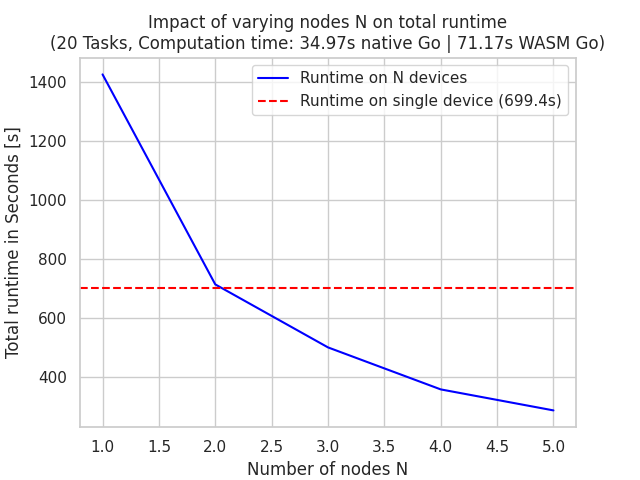
\includegraphics[width=.48\linewidth]{gfx/figures/Theory_A.png}
   } 
   \subfloat[Variable amount of tasks T]{
     \label{fig:background:theoryB}
     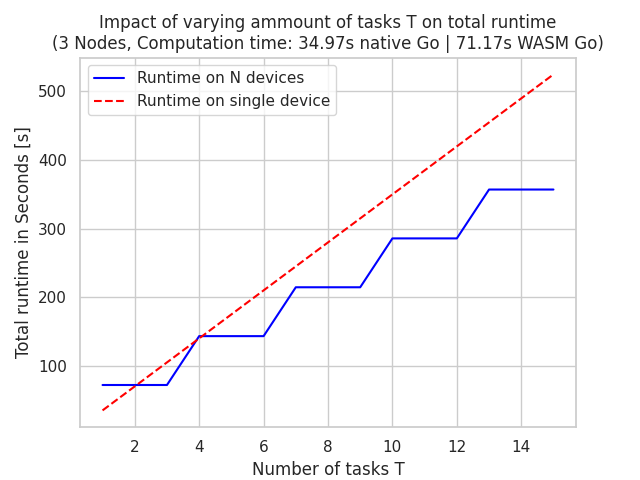
\includegraphics[width=.48\linewidth]{gfx/figures/Theory_B.png}
   }
   \caption{Visualizing the Total Computation Time for an Estimated Example Case}
   \label{fig:background:theoryplot}
\end{figure}
~\\
The graph in \autoref{fig:background:theoryA} represents the total runtime, on the y-axis in seconds, as a function of the number of nodes $N$ in the network, on the x-axis. The red dotted line displays the performance of a single machine $t_{ExSeq}$, while the blue line illustrates the performance of the volunteer computing network $t_{ExDist}$. The total number of all tasks $T$ is set to 20. This plot reveals that the volunteer network achieves a faster total computation time than a single device, if three or more nodes are availabile in the network. The total runtime $t_{ExDist}$ is already by 30\% faster than $t_{ExSeq}$ when the workload is distributed to three nodes.

The other graph in \autoref{fig:background:theoryB} displays the total runtime on the y-axis in seconds as a function of the number of tasks $T$ on the x-axis. The red dotted line represents again $t_{ExSeq}$ of a single device and the blue line $t_{ExDist}$ of the volunteer computing network. The number of nodes $N$ is set to three. This plot demonstrates that the volunteer network achieves faster total computation time than a single device when the workload $T$ consists of more than two tasks. The performance gain grows exponentially as the number of tasks increases. Furthermore, it can be concluded that the total computation time $t_{ExDist}$ of the volunteer network only increases when the number of tasks $T$ and the number of nodes $N$ have no common divisor. However, it is crucial to note that the network will have a longer computation time in every scenario with only one task, as a single task cannot be executed in parallel.

Both plots show, that the total computation time $t_{ExDist}$ is already almost even to the threshold value of $t_{ExSeq}$ if the volunteer network has two participating nodes and faster if there are three or more nodes. This holds true even if the computation time $t_{C}$ of a single task is twice as fast on a native system as measured in the browser environment. This proves that the approach of distributing the workload has a performance gain in this theoretical example, if multiple nodes participate in the volunteer computing network. 

However it needs to be considdered, that if there is only one or two node in the network this approach will already be slower in this example due to the initial offset time, the additional network latency and the higher computation time for each individual task.

\section{Related Work}
\label{sec:background:related_work}
The idea of volunteer computing has been established for a long time. The earliest concept of volunteer computing started already back in 1996 \cite{relatedwork:boinc1}. This section introduces relevant projects in this field, which have been used in the past or are currently in active use and maintenance.

\subsection{BOINC}
\label{subsec:background:related_work:boinc}
\ac{BOINC} is an open-source middleware system for volunteer computing, which utilizes consumer devices for scientific computing. It addresses key challenges in distributed computing, such as dealing with untrusted, unreliable, and heterogeneous computing resources, validating results from potentially malicious hosts, and supporting diverse applications and computing environments. \cite{relatedwork:boinc1}

The BOINC architecture consists of server components, including a database and job scheduler, and client software comprising a core client, GUI, and screensaver. Communication between clients and servers is facilitated through HTTP-based RPCs. BOINC employs replication-based validation and adaptive replication to ensure result integrity while minimizing overhead. The system also implements sophisticated scheduling policies both on the client and server sides to optimize resource allocation and job dispatch. \cite{relatedwork:boinc1}

BOINC has been successful in supporting numerous scientific projects and providing substantial computing power. \cite{relatedwork:boinc1}

\subsection{SETI@home}
\label{subsec:background:related_work:seti}
\ac{SETI} at home (\ac{SETI}@home) represents a pioneering project in the field of distributed and volunteer computing. It utilises the resources of volunteer computers worldwide to analyze radio telescope data in search of extraterrestrial intelligence. Data from the Arecibo radio telescope is divided into smaller chunks which are distributed to volunteer computers for processing. The system is designed to identify several types of patterns in radio signals that could indicate an artificial origin. These anormalies are spikes, Gaussians, pulsed signals, and triplets in the collected radio data. \cite{relatedwork:seti}

Back in the year 2002, \ac{SETI}@home had engaged over 3.8 million participants across 226 countries, achieving an average computing power of 27.36 teraFLOPS \cite{relatedwork:seti}.

\ac{SETI}@home demonstrated the viability of large-scale public-resource computing and identified key factors that make tasks suitable for this approach:
\begin{itemize}
  \item High computing-to-data ratio
  \item Independent parallelism
  \item Error tolerance
  \item Ability to attract public interest
\end{itemize}
The success of \ac{SETI}@home not only advanced scientific research but also increased public awareness and involvement in scientific participation. This project laid therefore the groundwork for future volunteer computing projects and frameworks. \cite{relatedwork:seti}

\subsection{XtremWeb}
\label{subsec:background:related_work:xtremweb}
XtremWeb is an experimental Global Computing platform designed to harness idle computing resources connected to the Internet for high-throughput computing. The system aims to provide a platform for experimenting with Global Computing capabilities and addressing issues such as scalability, heterogeneity, availability, fault tolerance, security, and usability in massively distributed computing environments. \cite{relatedwork:xtremweb}

The architecture of XtremWeb consists of three main components:
\begin{enumerate}
  \item Workers: These are volunteer PCs that execute tasks. They are implemented primarily in Java for portability, with native code used for OS-specific functions. Workers monitor resource availability based on user-defined policies and support multiple platforms, including Linux and Windows.
  \item Servers: These manage tasks and applications. The server design is modular, with components for application pool, job pool, accounting, and scheduling. Servers can be clustered for increased throughput and support specialization for tasks such as dedicated result collection.
  \item Clients: These submit tasks to the system.
\end{enumerate}
XtremWeb employs a two-part scheduling system:
\begin{enumerate}
  \item Dispatcher: Selects tasks from the pool based on application priorities.
  \item Scheduler: Assigns tasks to workers.
\end{enumerate}
The default scheduling policy of XtremWeb is FIFO and XtremWeb implements a timeout to enable rescheduling of aborted tasks \cite{relatedwork:xtremweb}.

Furthermore XtremWeb implements a worker-initiated communication protocol, which facilitates easier deployment through firewalls. This protocol consists of the four main requests: \emph{hostRegister}, \emph{workRequest}, \emph{workAlive}, and \emph{workResult}. \cite{relatedwork:xtremweb}

XtremWeb has been successfully applied to various projects in the past. Thes include the Pierre Auger Observatory for studying high-energy cosmic rays. In this application, XtremWeb was used to run the \ac{AIRES} program by partitioning large simulations into smaller subtasks. \cite{relatedwork:xtremweb}

In summary, XtremWeb provides a flexible and robust platform for experimenting with Global Computing concepts. Its approach and concept has some similarities to WebCrowd. The original XtremWeb project seems to be not maintained since its development in the early 2000s.

\subsection{EGEE}
\label{subsec:background:related_work:egee}
Initiated on April 1, 2004, \ac{EGEE} was a two-year project within a planned four-year program, involving 71 partners from Europe, Russia, and the United States \cite{relatedwork:egee}. The project's primary objectives were to establish a seamless European grid infrastructure for scientific research, provide production-level grid services, and re-engineer grid middleware for enhanced robustness and scalability \cite{relatedwork:egee}.

The infrastructure of \ac{EGEE} was built upon the EU Research Network GEANT, leveraging expertise from previous initiatives such as EU DataGrid, UK e-Science, INFN Grid, Nordugrid, and US Trillium. The project aimed to expand its computational capabilities from an initial 3000 CPUs at 10 sites to 10000 CPUs across 50 sites by the end of 2005 \cite{relatedwork:egee}.

\ac{EGEE} focused on two primary pilot applications: 
\begin{itemize}
  \item The \ac{LCG} for high-energy physics data analysis.
  \item Biomedical Grids addressing challenges in genomic database mining and medical database indexing
\end{itemize}
The project focused on re-engineering existing middleware to address issues from first-generation implementations and ensure adherence to \ac{OGSA} standards. This approach aimed to enhance the reliability and scalability of the grid infrastructure \cite{relatedwork:egee}.

In conclusion, the \ac{EGEE} project represented a significant effort to transform grid computing from a research concept into a practical infrastructure to support "e-science" across Europe.

\subsection{WebAssembly for Edge Computing}
\label{subsec:background:related_work:wasmedgecomputing}
The work from \citeauthor{relatedwork:wasmedgecomputing} \cite{relatedwork:wasmedgecomputing} investigates WebAssembly as a promising solution for edge computing challenges, particularly addressing the crucial requirements of portability and migratability for such applications. This work builds upon previous research in edge computing virtualization while introducing novel perspectives on using WebAssembly as an enabling technology for portable and migratable edge applications. Their comprehensive analysis demonstrates WebAssembly's capabilities in achieving near-native performance while maintaining platform independence, which proposes a significant advancement compared to traditional virtualization approaches. In their work the authors present a systematic evaluation of different WebAssembly execution environments, including browser-based implementations and standalone runtimes, focusing on the performance to portability trade-off. 

Their findings highlight WebAssembly's potential as a lightweight alternative to conventional virtual machines or container based approaches in edge computing scenarios \cite{relatedwork:wasmedgecomputing}. However, they identified that WebAssembly is currently lacking migratability features, compared to virtual machines and containers, to make it a complete solution for edge computing environments \cite{relatedwork:wasmedgecomputing}. Depending on the migration scenario they provide ideas for further actions or development to utilize WebAssembly.

\subsection{Dynamic Mobile Device Clusters in
Edge Femtoclouds}
The work from \citeauthor{relatedwork:mobilecloud} \cite{relatedwork:mobilecloud} explored the concept of Edge Femtoclouds, which demonstrated significant performance improvements through collaborative mobile edge computing \cite{relatedwork:mobilecloud}. Their experimental results show that Edge Femtoclouds can reduce job completion time by up to 26\% compared to traditional cloud computing approaches, with their novel checkpointing mechanism further improving efficiency by an additional 31\% \cite{relatedwork:mobilecloud}. The authors developed a comprehensive system architecture incorporating cloud-based controllers, mobile device helpers, and job managers, successfully addressing the challenges of device churn and system stability. 

Their prototype demonstrated robust performance across varying job arrival rates \cite{relatedwork:mobilecloud}. While highlighting the benefits of reduced latency and network congestion, their findings also identified key challenges including the need for sufficient device participation and robust security measures \cite{relatedwork:mobilecloud}. The work presents Edge Femtoclouds as a cost-effective alternative to dedicated edge servers, though noting the importance of developing appropriate incentive mechanisms for device owners.

They stated that the support of heterogen devices is a important feature for such a application, due to the heterogeneous characteristic of the mobile device environment \cite{relatedwork:mobilecloud}. However the implemented prototype that was build in their work was only supporting android devices as a proof of concept.
\chapter{Methodology}
\label{ch:methodology}
The overall process of developing the WebArgo platform presented in this work consited of the following steps:
\begin{enumerate}
  \item Theoretical design of the platforms Architecture
  \item Development of a Proof of Concept prototype
  \item Development process from the prototype to the WebArgo platform
  \begin{itemize}
    \item Implementation of \acs{API} and web interface
    \item Usage of generic job and task entities to support any kind of custom job
    \item Add WebAssembly Support for multiple programming languages
    \item Implement support for various output datatypes (primitiv datatypes, lists, files as binary)
  \end{itemize}
  \item Deployment of the web application
  \begin{itemize}
    \item Orchestrate all components of the WebArgo platform with Docker Compose \cite{conclusion:docker}
    \item Host the project on a cloud services (\emph{openstack} from h\_da)
    \item Implement user entity with specific user roles to enable security
    \item Implement security measures through authentication \& authorization
  \end{itemize}
  \item Enhance robustness of the platform
  \begin{itemize}
    \item Implement system recovery measures and persistence of critical data
    \item Adjust scheduling algorithm to ensure the completion of jobs, even when workers are unreliable
    \item Eliminate bugs through testing the application
  \end{itemize}
  \item Implement the visualization of the Mandelbrot set in multiple languages as the benchmark job
  \item Evaluation of the platform through multiple experiments 
\end{enumerate}
The following content of this chapter enumerates and describes all the technologies, frameworks, and tools utilized in the development of the volunteer computing platform, along with the reasoning for their selection. Each section provides a detailed explanation of these components, establishing a foundation for the following \autoref{ch:implementation} which focuses on the implementation. Additionally, all entities are listed and described in \autoref{sec:methodology:entities} to define all specific terms used in the subsequent chapters.

\section{Entities}
\label{sec:methodology:entities}
This section describes all entities and establishes the terms used to describe the processes in this work.

\subsection{Job}
\label{subsec:methodology:entities:job}
The job entity represents a problem to be processed or solved using the platform. The platform is designed to handle multiple jobs while each job is a unique object. The State of a job can have one of the following values:
\begin{itemize}
  \item PENDING
  \item ACTIVE
  \item RUNNING
  \item STOPPED
  \item DONE
\end{itemize}
\begin{figure}[htbp]
  \centering
  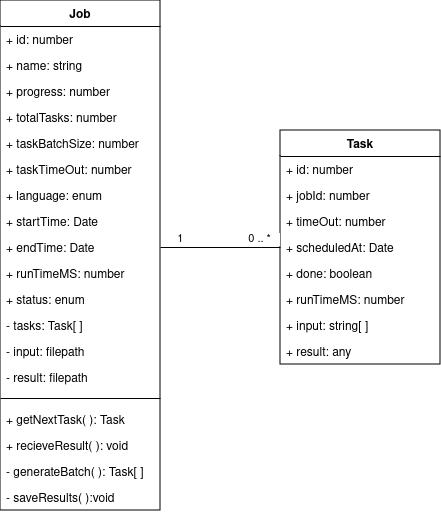
\includegraphics[width=0.75\textwidth]{gfx/figures/Job-Task.png}
  \caption{\acs{UML} Class Diagram: Job \& Task}
  \label{fig:methodology:job-task}
\end{figure}
\autoref{fig:methodology:job-task} illustrates the \ac{UML} class diagram for the job entity on the left side, lisitng all important attributes and methods of a job. The language attribute defines the programming langugae of the source code that has been compiled to a WebAssembly binary file.

\subsection{Task}
\label{subsec:methodology:entities:task}
Each job is divided into multiple equally sized tasks. These tasks are distributed to the worker nodes of the platform. Tasks are unique objects, each holding the specific input parameters that describe the particular portion of the job to which the task is assigned. \autoref{fig:methodology:job-task} displays the \ac{UML} class diagram for the task entity on the right side. The relationship between the job and task entities is defined as One-to-Many, meaning a job can consist of multiple tasks, but each task is always assigned to a single job.

\subsubsection{Batch}
\label{ssubsec:methodology:entities:task:batch}
A batch is defined to be a subset of tasks, wich are all assigned to the same job.

\subsection{Client}
\label{subsec:methodology:entities:client}
\begin{figure}[htbp]
  \centering
  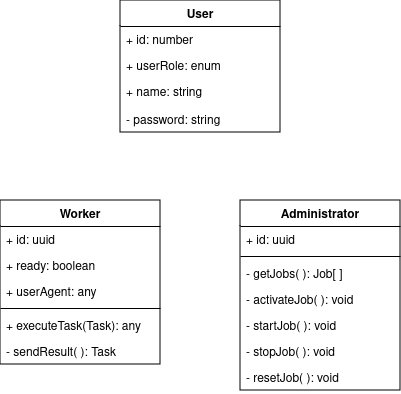
\includegraphics[width=0.75\textwidth]{gfx/figures/Client.png}
  \caption{\acs{UML} Class Diagram: User - Worker \& Administrator}
  \label{fig:methodology:client}
\end{figure}
~\\
A client represents a node that accesses the platform. The actions a client can perform are determined by the user role assigned to its user. This user role can either have the value \emph{User} for limited access or \emph{Admin} for full access to all features. \autoref{fig:methodology:client} displays the \ac{UML} class diagram for the user entity at the top of the illustration.

\subsubsection{Worker}
\label{ssubsec:methodology:entities:client:worker}
Workers are clients that voluntarily donate their computing power to support an active job. Therfore they receive tasks from the current batch sent by the server (\autoref{subsec:methodology:entities:Server}), compute these tasks, and return the corresponding results back to the server. \autoref{fig:methodology:client} presents the \ac{UML} class diagram of the worker entity on the left side, listing all relevant attributes and methods. As workers connect to the server via web browsers, the browser's user agent is utilized to individually characterize each worker. This so called browser user agent can be accessed inside the clients browser environment and provides information about the client's hardware resources and operating system.

\subsubsection{Administrator}
\label{ssubsec:methodology:entities:client:admin}
An administrator client can perform the same actions as a worker, but also has additional capabilities. Only administrators have the ability to set or change the state of jobs and to oversee the progress of all jobs. \autoref{fig:methodology:client} illustrates the \ac{UML} class diagram of the administrator entity on the right side.

\subsection{Server}
\label{subsec:methodology:entities:Server}
The server is used as the central component to maintain the network. Each client intending to connect to the network must establish a connection with the server.

Additionally the server is responsible for scheduling and distributing the tasks to all workers. It also persistently stores each job along with all results of its corresponding tasks.

\section{Database}
An object-relational database system was identified to fulfill the platform's requirements, as these systems typically offer high performance capabilities and the entities described in the previous sections can be represented with an object-relational database schema.

PostgreSQL is an open source object-relational database system that has been actively developed for more than 35 years \cite{methodology:db}. Therefore it has gained a strong reputation for reliability, feature robustness, and performance \cite{methodology:db}, hence PostgreSQL was selected as the database management system for this implementation.

\section{Frameworks}
\label{sec:methodology:frameworks}
This section introduces the frameworks selected for the development of the web application. The following criteria were used to guide the selection of a suitable framework for the backend as well as the frontend:
\begin{itemize}
    \item The framework is well-tested and provides a stable \ac{LTS} version.
    \item The framework is popular among web developers.
\end{itemize}

\subsection{Backend}
\label{subsec:methodology:frameworks:backend}
It was crucial for the backend framework to be popular among web developers. Working with a popular framework improves the development process by ensuring the availability of detailed educational resources online as well as various online support forums. Additionally, a widely used framework increases the likelihood that the platform can be maintained or further extended by other programmers.
\begin{figure}[htbp]
 \centering
 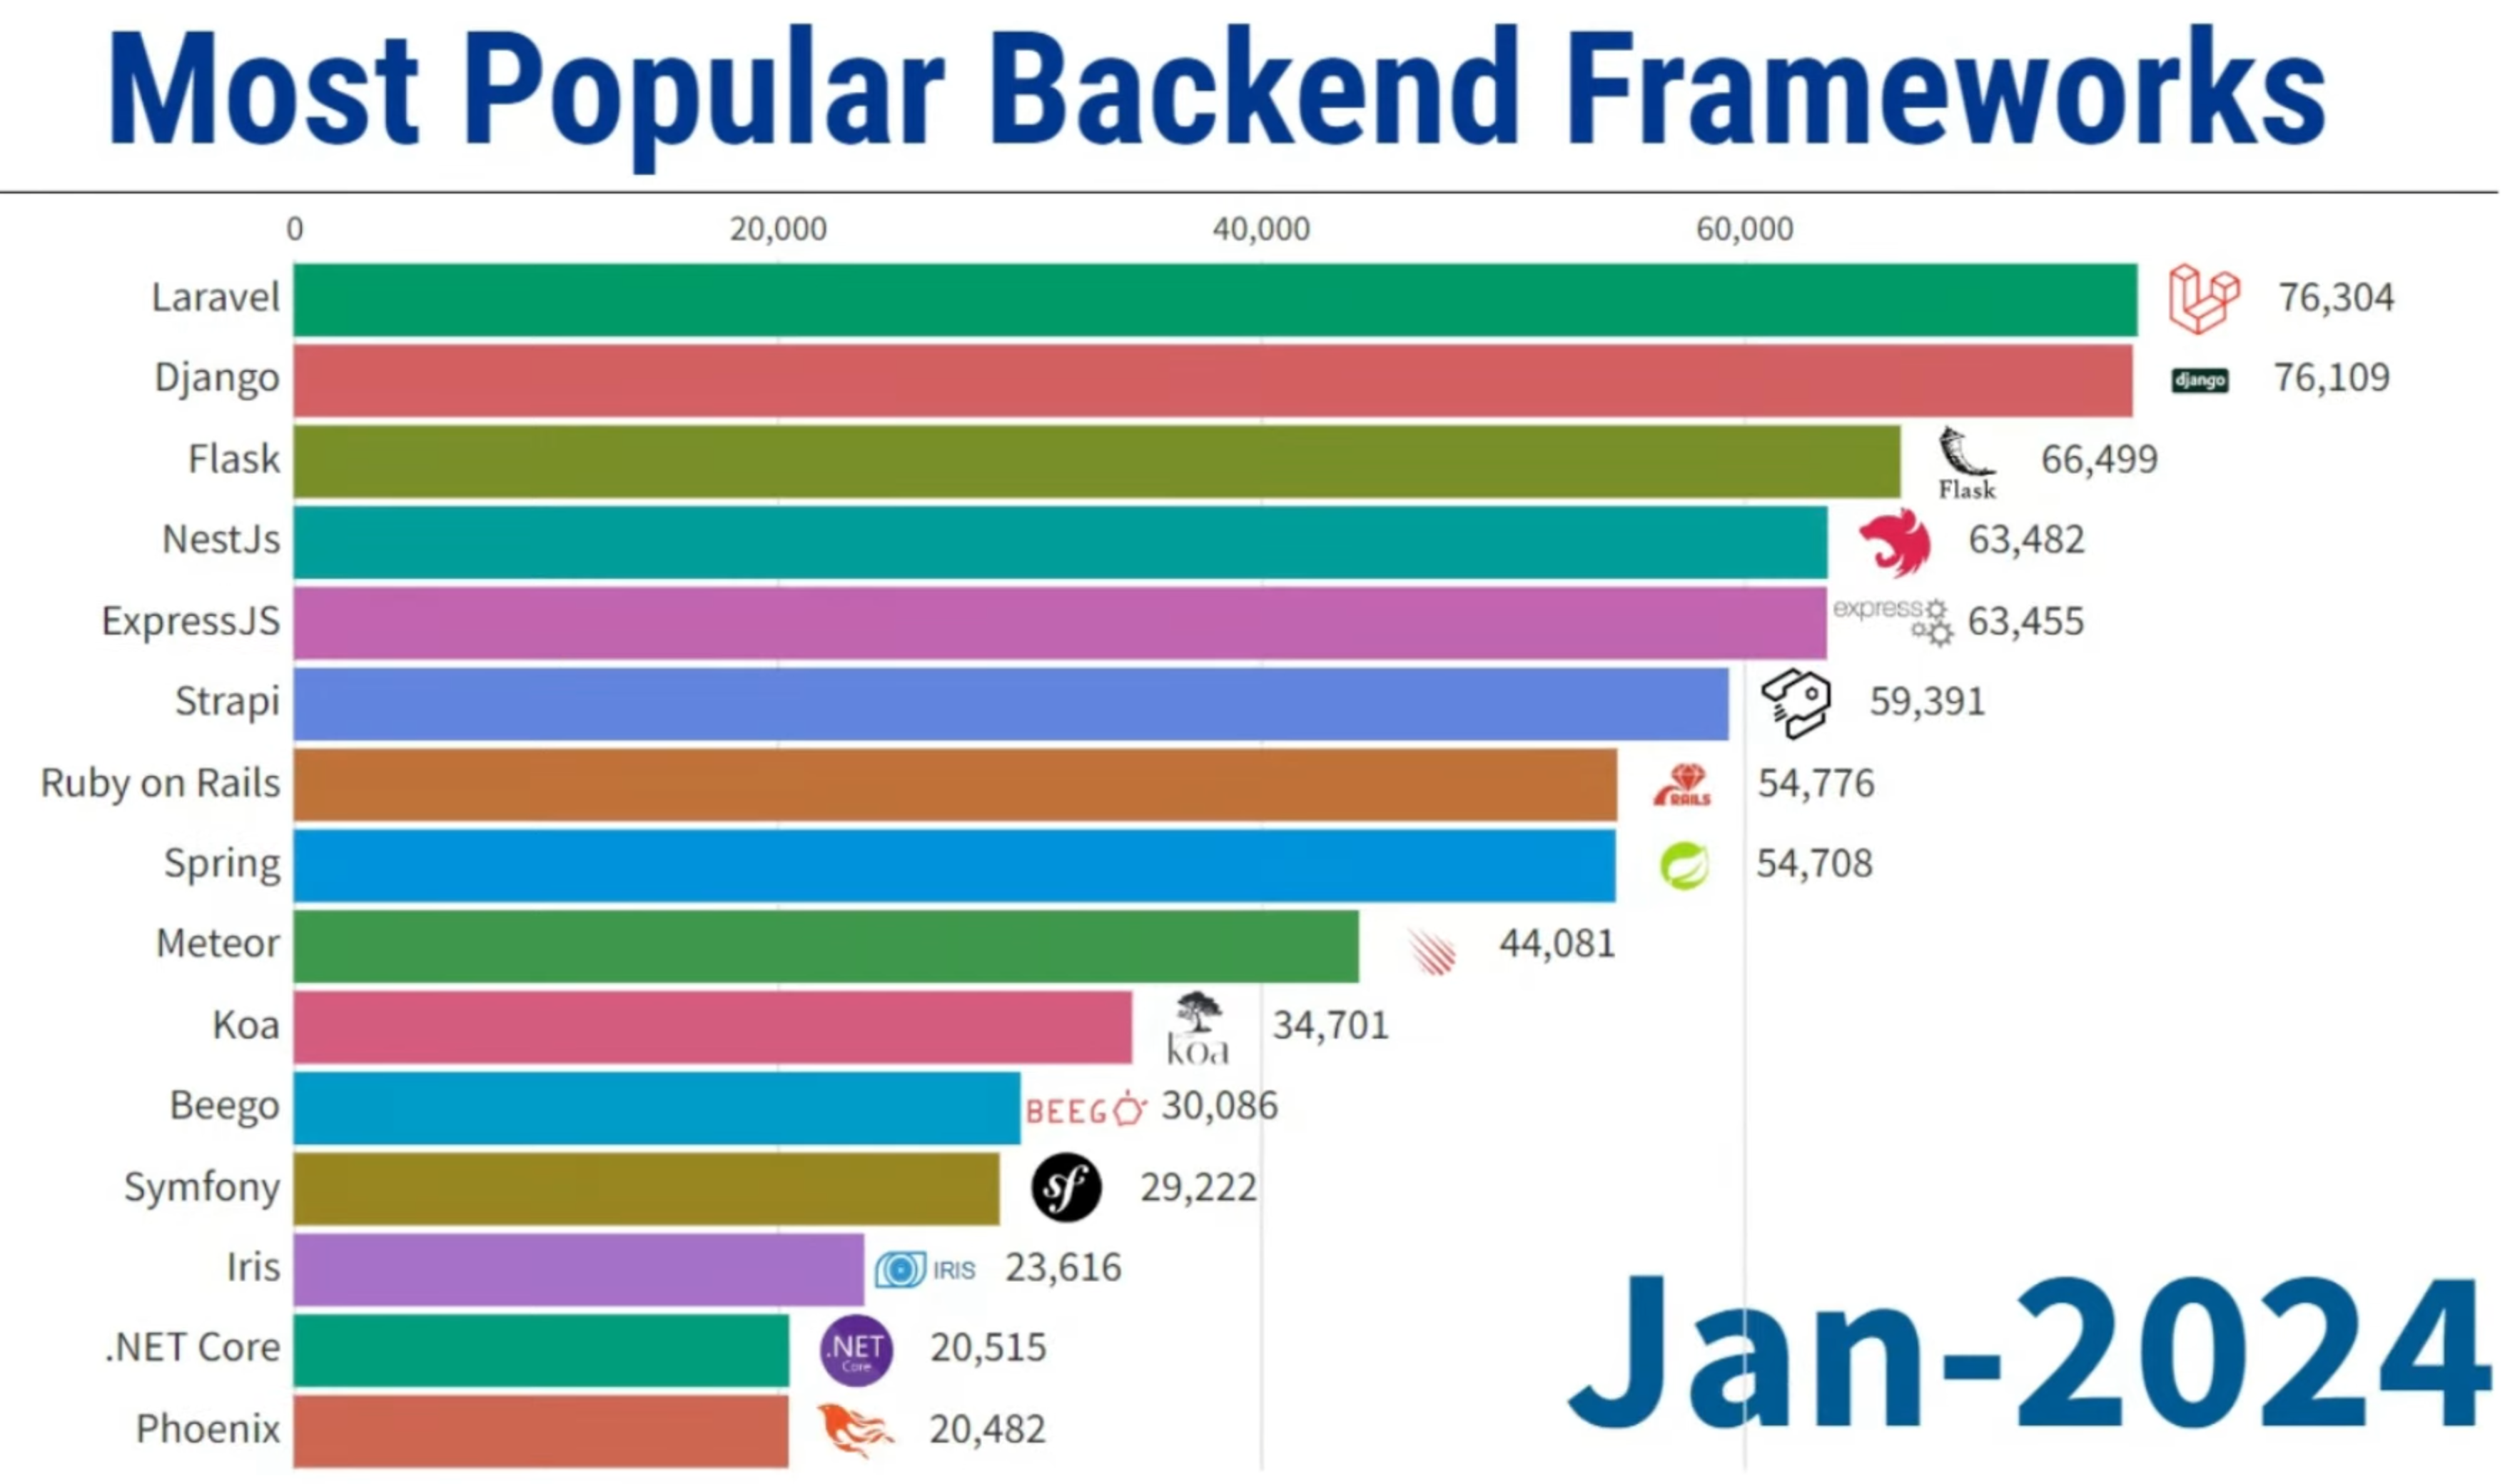
\includegraphics[width=0.95\textwidth]{gfx/figures/Popular_BE.png}
 \caption{Most Popular Backend Frameworks (Jan 2024) by GitHub Stars \cite{backend:popularity}}
 \label{fig:methodology:popularBE}
\end{figure}
~\\
The 15 most popular backend frameworks of January 2024 are displayed in \autoref{fig:methodology:popularBE}. The popularity for each framework of this list is calculated by the number of GitHub Stars from repositories listed in a GitHub Archive \cite{backend:popularity}. The selection options of the backend framework where based on this popularity list.

In addition to the previously stated criteria, the selected backend framework needed to meet specific performance requirements. It was essential for the framework to efficiently handle multiple connected clients with minimal latency. Furthermore, the framework's internal computation speed was critical, particularly for preparing input arguments for each task and managing task scheduling across all clients. The goal was to reduce overhead as much as possible to ensure high performance.
\begin{figure}[htbp]
  \myfloatalign
  \subfloat[Best fortunes responses per second (2023-10-17) \cite{backend:benchmark2}]{
    \label{fig:methodology:benchmark2BE}
    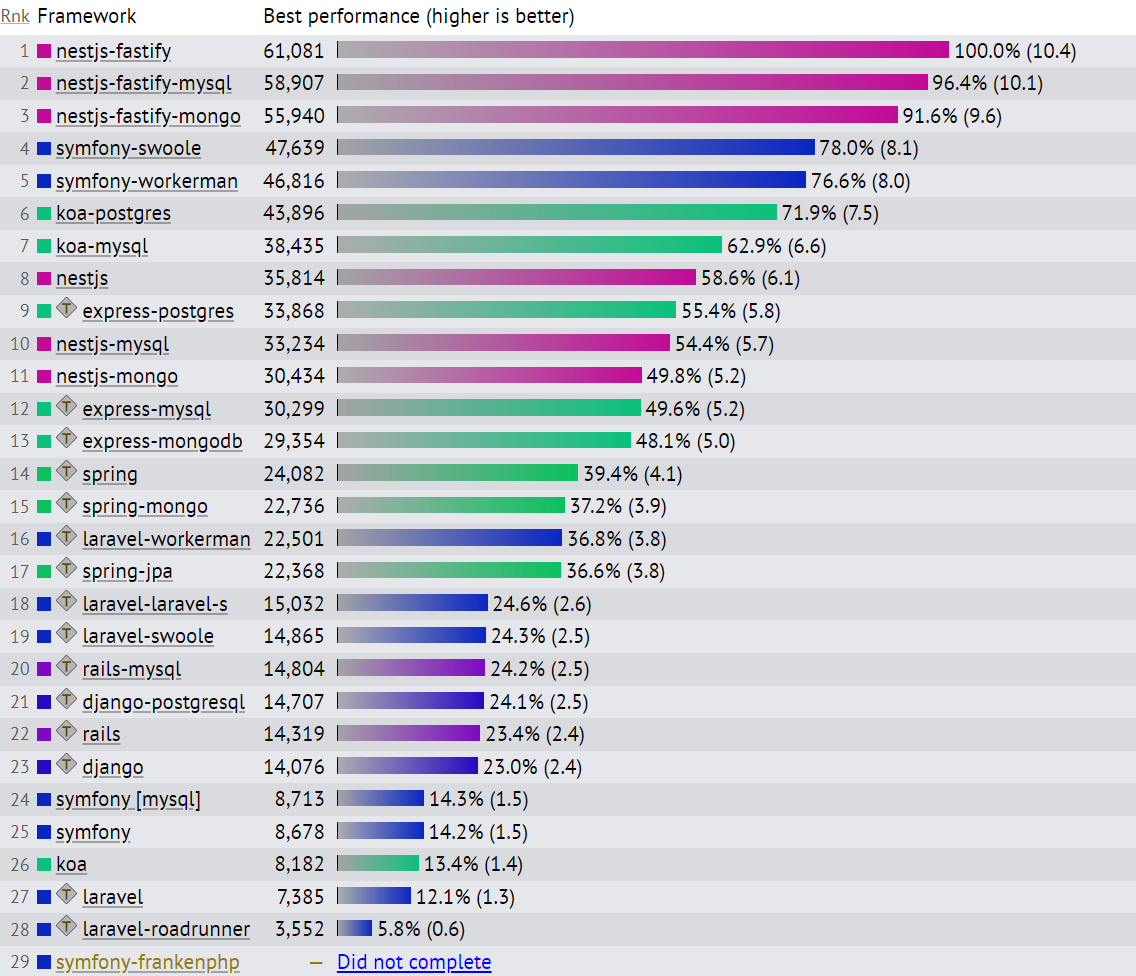
\includegraphics[width=.95\linewidth]{gfx/figures/Benchmark2_BE.png}
  }
  \caption{Most Popular Backend Frameworks from \autoref{fig:methodology:popularBE} Ranked by Performance.}
  \label{fig:methodology:benchmarkBE}
\end{figure}
\begin{figure}[htbp] \ContinuedFloat
  \myfloatalign
  \subfloat[Requests/Second (2024-06-25) \cite{backend:benchmark1}]{
     \label{fig:methodology:benchmark1BE}
     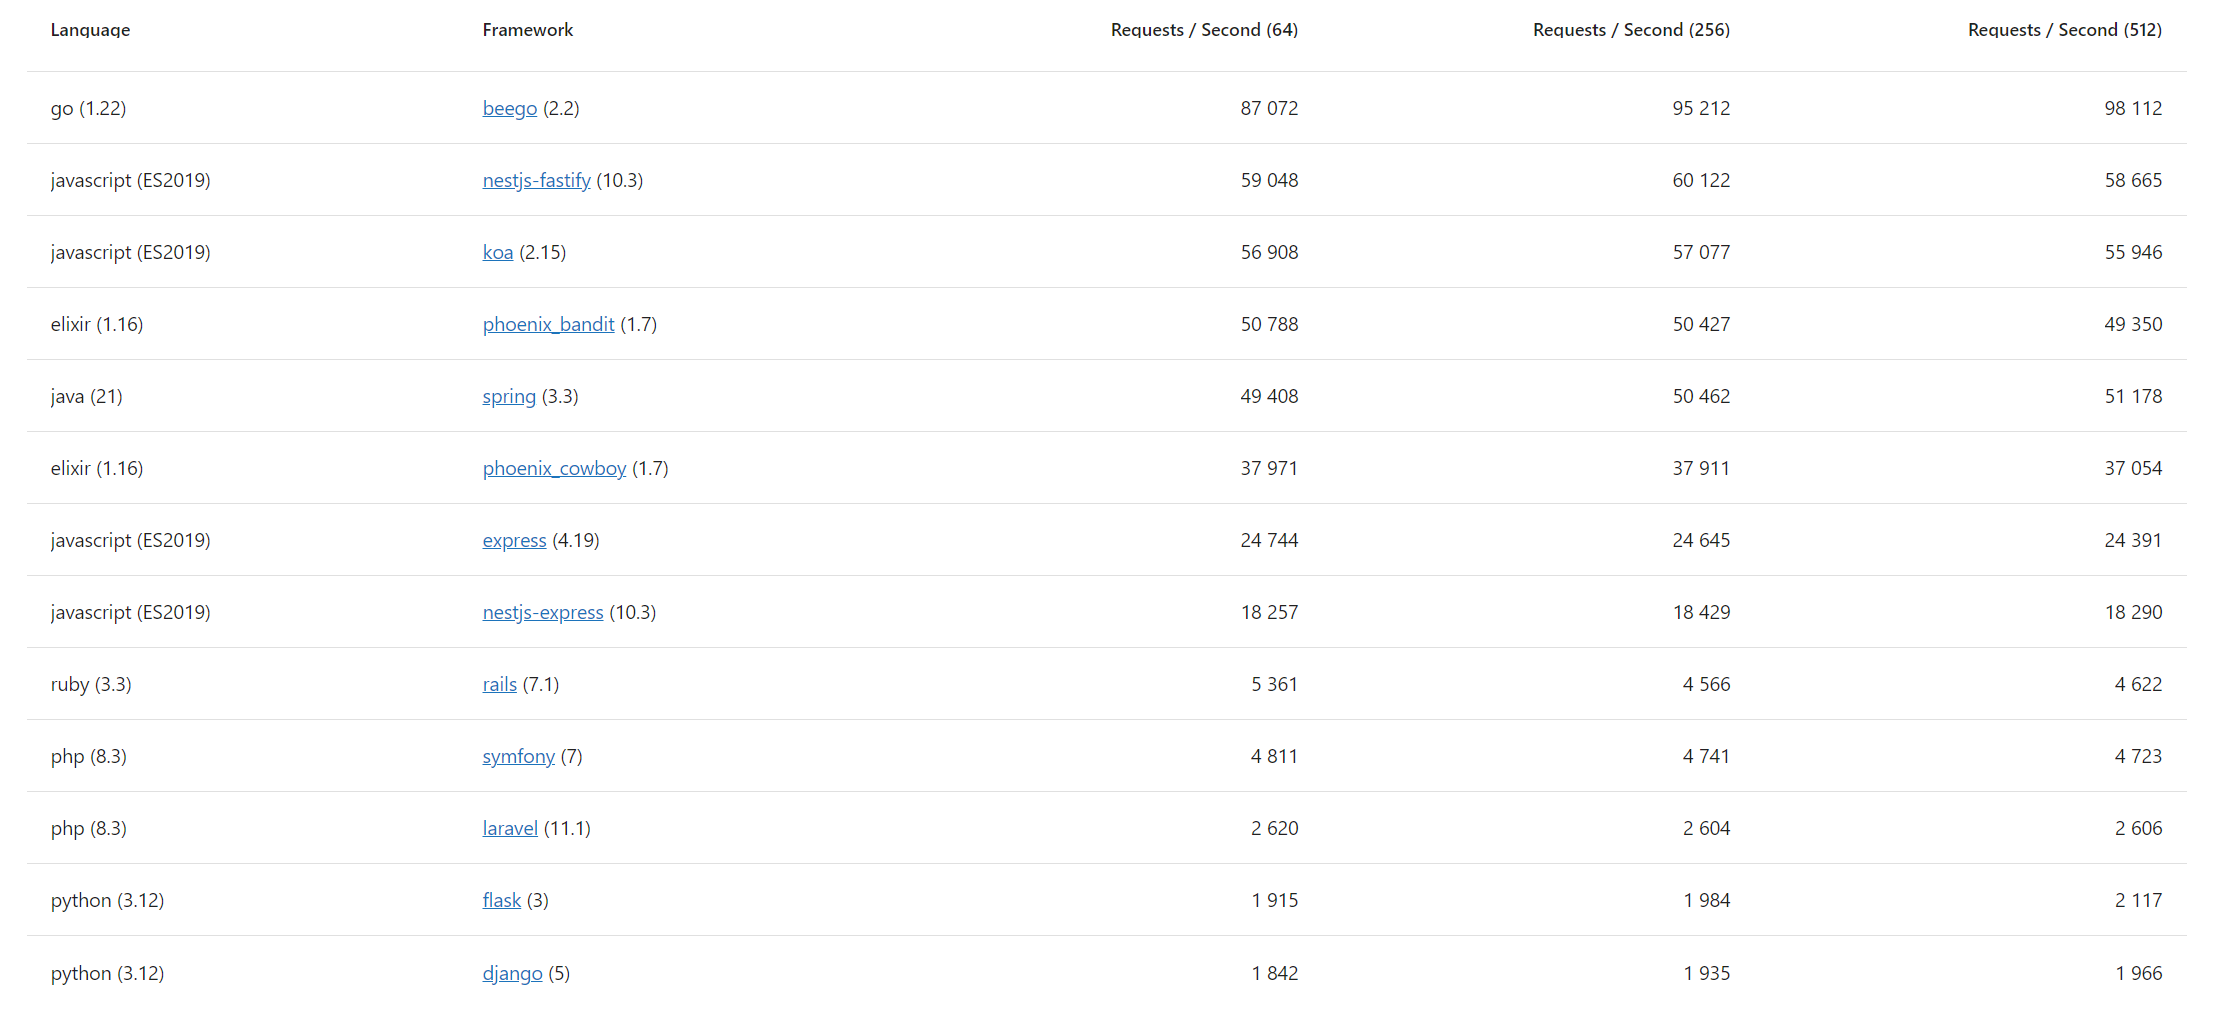
\includegraphics[width=.75\linewidth]{gfx/figures/Benchmark1_BE.png}
   }
   \caption{Most Popular Backend Frameworks from \autoref{fig:methodology:popularBE} Ranked by Performance.}
   \label{fig:methodology:benchmarkBE}
\end{figure}
~\\
To identify a high-performance framework, the most popular backend frameworks listed in \autoref{fig:methodology:popularBE} were compared by using two independent benchmark sources. The results of these benchmarks are presented in \autoref{fig:methodology:benchmarkBE}, where the frameworks are ranked from top to bottom based on their performance. It is important to note that some frameworks from the list in \autoref{fig:methodology:popularBE} where not part of these specific benchmarks. Both benchmark sources simulated numerous clients sending requests to each backend and measuring the number of successful responses per second in order to determine the performance \cite{backend:benchmark1, backend:benchmark2}.

Finally, NestJS \cite{methodology:nestjs} with Fastify was selected as the backend framework. It performed exceptionally well in both benchmarks shown in \autoref{fig:methodology:benchmarkBE} and is also a popular choice among developers.

\begin{figure}[htbp]
  \centering
  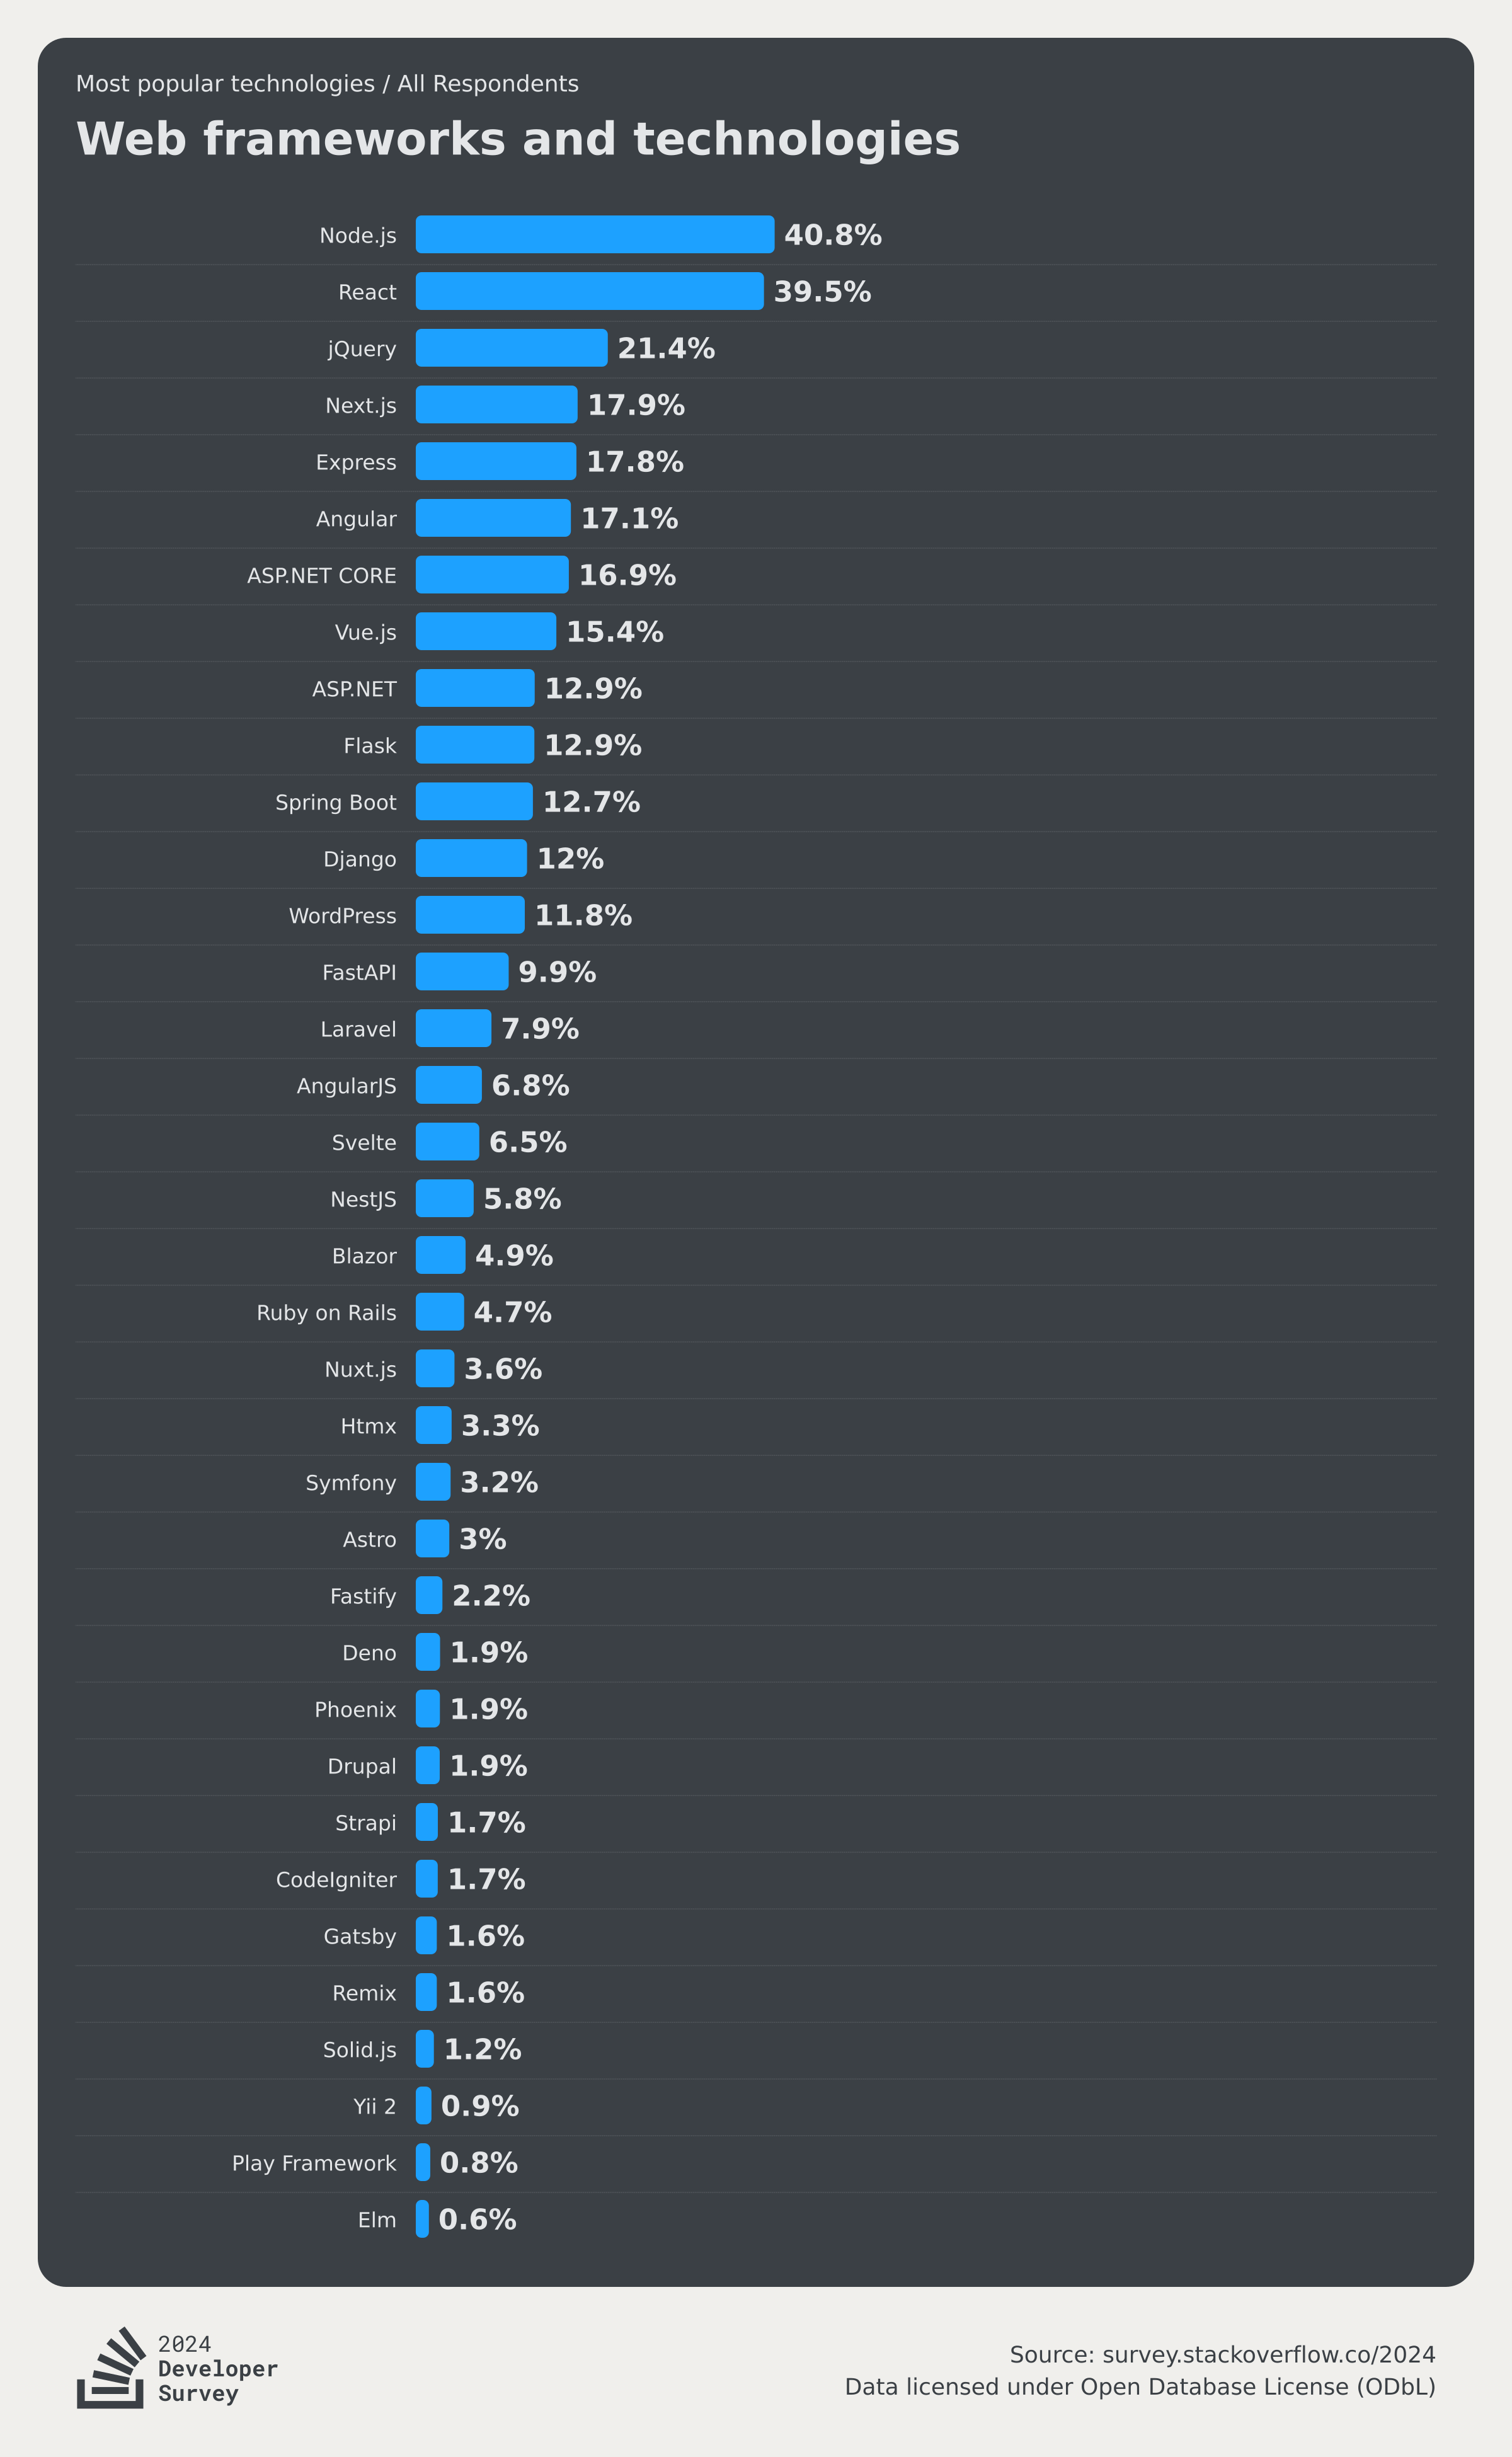
\includegraphics[width=0.95\textwidth]{gfx/figures/FrameworkSurvey2024.png}
  \caption{Most Used Web Frameworks and Technologies in 2024 (Developer Survey from Stack Overflow) \cite{frontend:popularity}}
  \label{fig:methodology:popularFE}
\end{figure}
\clearpage

\subsection{Frontend}
\label{subsec:methodology:frameworks:frontend}
The criteria stated in \autoref{sec:methodology:frameworks} also applied for the selection of a framework for the frontend. \autoref{fig:methodology:popularFE} shows the 36 most used frameworks among web developers in July 2024 \cite{frontend:popularity}. This statistic has been collected by Stack Overflow and is the result of a survey. In this survey web developers have been asked which web frameworks and web technologies they had been working with in the past year, and which do they want to work in over the next year \cite{frontend:popularity}. The two most popular options are, by far, Node.js and React with each around 40\% of votes. While Node.js is mainly used for backend development React is a JavaScript library used for frontend development. This is qualifying React as the choice of technology for the frontend development. Ranking fourth in \autoref{sec:methodology:frameworks} is Next.js with 17.9\% of votes. Next.js is a web framework based on React \cite{methodology:nextjs} and according to the survey the most popular React web framework in the year 2024. Therfore Next.js was selected as the framework for frontend development.

\section{WebAssembly}
\label{sec:methodology:wasm}
WebAssembly \cite{methodology:wasmW3C} is a key technology utilized in the implementation of WebArgo, offering several advantages for distributed or edge computing \cite{relatedwork:wasmedgecomputing}. It provides near-native performance, while maintaining platform independence \cite{methodology:wasm, methodology:wasmW3C, relatedwork:wasmedgecomputing}. 

WebAssembly is a low-level binary instruction format designed to serve as a compilation target for high-level programming languages \cite{methodology:wasm, methodology:wasmW3C, methodology:wasm2}, that promisses near-native performance execution in web browsers \cite{methodology:wasm, methodology:wasmW3C, relatedwork:wasmedgecomputing}. It employs a stack-based virtual machine architecture, operates in a memory-safe sandboxed environment, and interacts with JavaScript of the browser environment through a defined \ac{API} \cite{methodology:wasm, methodology:wasmW3C, methodology:wasm2, methodology:wasmdocu}. A compiled WebAssembly is particularly effective for computationally intensive tasks in the browser \cite{methodology:wasm2, methodology:wasmW3C} like image processing, game engines, or cryptographic operations.

The flexible features of platform independence and support of multiple high-level programming languages makes WebAssembly a fantastic choice for the WebArgo platfrom.
\\~\\
Furthermore, WebAssembly is maintaining the browsers inherent security model \cite{methodology:wasmW3C, methodology:wasm2, methodology:wasmdocu}. This is preventing any application to read and write files or to access device hardware such as cameras or microphones without explicit user permissions. Therfore WebArgo is ensuring a higher security for worker nodes than other volunteer computing applications, which require the installation of third-party software directly to the machine. This directly addresses the privacy and security concerns revealed by the study of \citeauthor{intro:volunteerStudy} \cite{intro:volunteerStudy} to increase the potential pool of participating workers.
\clearpage
\begin{figure}[htbp]
  \centering
  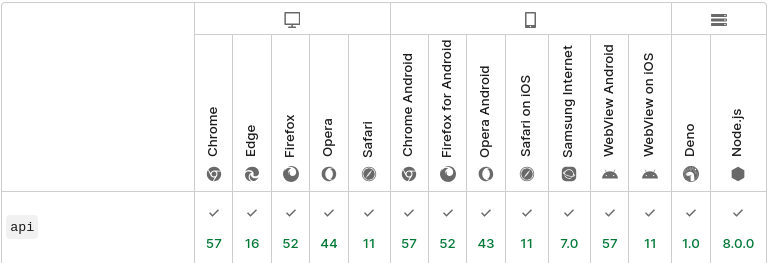
\includegraphics[width=0.95\textwidth]{gfx/figures/webassembly-browsercompability.png}
  \caption{Browser Compatibility: WebAssembly \cite{methodology:wasmdocu}}
  \label{fig:methodology:wasm}
\end{figure}
~\\
\autoref{fig:methodology:wasm} displays the browser compatibility of WebAssembly with multiple major browsers \cite{methodology:wasmdocu}. The check mark indicates WebAssembly support and the green number below marks the version since WebAssembly support was implemented. All browsers are sorted by desktop and mobile version. 

\subsection{emscriptren for C and C++}
\label{subsec:methodology:wasm:cpp}
The toolchain, used in this work, to compile C or C++ code into the WebAssembly binary format is emscripten. The team of emscripten already focused on the compilation of C and C++ code to \emph{asm.js} - a predecessor of WebAssembly - in the past \cite{methodology:emcc}. This compiler infrastructure has evolved to target the WebAssembly format, enabling the execution of native C/C++ applications in web browsers. Furthermore, emscripten provides the necessary JavaScript glue code to initialize the WebAssembly environment according to the compiled source code \cite{methodology:emcc}.

\subsection{Go}
\label{subsec:methodology:wasm:go}
The standard Go compiler inherently provides a option to directly target the WebAssembly format during the compilation process \cite{methodology:go}. This was utilized to support Go applications in WebArgo. Unlike emscripten, this compilation to WebAssembly is not producing a specific JavaScript glue code file for each Go application, however Go provides a general JavaScript glue code file suitable for all generated WebAssembly binaries \cite{methodology:go}. The files size of this general Go JavaScript glue code is surprisingly small compared to the JavaScript glue code generated by emscripten.

\subsection{Pyodie for Python}
\label{subsec:methodology:wasm:python}
Pyodide is described to be a port from CPython to WebAssembly/Emscripten \cite{methodology:pyodie}. It is a JavaScript library that provides a robust foreign function interface to compile python code to WebAssembly and execute it inside the browser environment \cite{methodology:pyodie}. Additionally it enables the installation and execution of Python packages inside the browser using micropip \cite{methodology:pyodie}. Also Pyodide promisses, that the executed Python code has full access to the Web \ac{API}s \cite{methodology:pyodie}, which is not an default feature of emscripten or Go.

Unfortunatly, Pyodide performed relatively slow compared to emscripten or Go during the testing of this work.

\section{WebSokets}
\label{sec:methodology:websokets}
WebSockets play a crucial role for the communication infrastructure of WebArgo. Different from standard \ac{HTTP} requests enable WebSockets a faster, bidirectional and full-duplex communication between clients and servers \cite{methodology:websockets1, methodology:websockets3, methodology:websockets2}. Unlike traditional \ac{HTTP} request-response patterns, WebSocket are establishing a persistent connections between client and server \cite{methodology:websockets3}, allowing real-time data transmission in both directions with minimal overhead after the initial handshake \cite{methodology:websockets3}. This protocol utilizes the ws:// or wss:// (secure) URI scheme and efficiently handles scenarios requiring live updates such as financial trading platforms, multiplayer games, or chat applications, with significantly reduced latency compared to polling mechanisms.

The real-time capability is leveraged for efficient task distribution, progress monitoring, and result collection in the implementation of the WebArgo platform. Additionally, is the bidirectional and full-duplex communication model extreamly usefull to handel the transmission of task and results between the server and workers. This replaces unperformant polling strategies and therfore enhances the performance of the communication process between server and workers.
\begin{figure}[htbp]
  \centering
  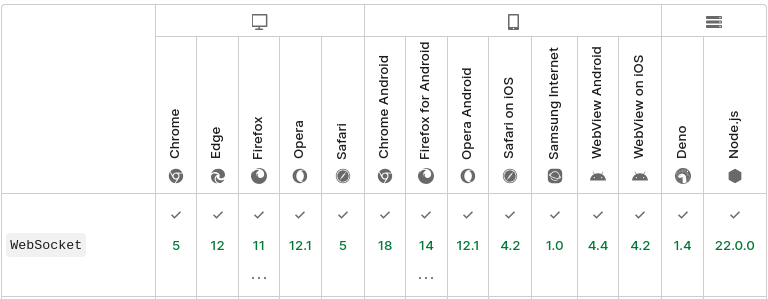
\includegraphics[width=0.95\textwidth]{gfx/figures/websocket-browsercompability.png}
  \caption{Browser Compatibility: WebSocket \cite{methodology:websockets1}}
  \label{fig:methodology:websocket}
\end{figure}
~\\
\autoref{fig:methodology:websocket} displays the browser compatibility of WebSocket with multiple major browsers \cite{methodology:websockets1}. The check mark indicates WebSocket support and the green number below marks the version since WebSocket support was implemented. All browsers are sorted by desktop and mobile version. 

\subsection{Socket.IO}
Socket.IO \cite{methodology:websockets2} is a popular JavaScript library that implements the usage of WebSockets on both the server and client side. NestJS \cite{methodology:nestjs}, the selected framework to implement the backend, has an inherent support of Socket.IO, using its concept of so called \emph{Gateways} \cite{methodology:nestjs}. Therfore the Socket.IO libary was selected to implement WebSocket inside the WebArgo platform.

\section{WebWorker}
\label{sec:methodology:webworker}
WebWorkers can be accessed through a specific JavaScript \ac{API}, enabling concurrent execution of scripts in background threads separate from the main browser UI thread \cite{methodology:webworkers}. These WebWorkers operate in an isolated context, communicating with the main thread through a message-passing interface, and therfore cannot directly access the \acs{HTML} \acs{DOM} of the web page \cite{methodology:webworkers}. 

This implementation of parallel processing through WebWorkers prevents the computationally intensive WebAssembly execution from blocking the user interface of a worker. This enables the worker to monitor the currently executed task and prevents an unpleasent user experience caused by an unexpectatly frozen screen. Furthermore, the WebWorker \ac{API} allows to create multiple WebWorkers in parallel. This feature could be used in the future to implement a browser based multi-threading solution for WebArgo.
\begin{figure}[htbp]
  \centering
  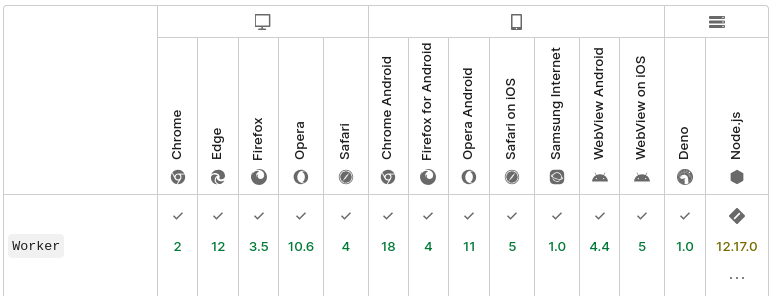
\includegraphics[width=0.95\textwidth]{gfx/figures/webworker-browsercompability.png}
  \caption{Browser Compatibility: WebWorker \cite{methodology:webworkers}}
  \label{fig:methodology:webworker}
\end{figure}
~\\
\autoref{fig:methodology:webworker} displays the browser compatibility of WebWorker with multiple major browsers \cite{methodology:webworkers}. The check mark indicates WebWorker support and the green number below marks the version since WebWorker support was implemented. All browsers are sorted by desktop and mobile version. 

\section{Benchmark: Visualizing the Mandelbrot set}
\label{sec:methodology:benchmark}
To benchmark the platform's performance, a computationally intensive job is implemented and executed across multiple connected workers. The total execution time is compared to the execution time of the same job on a single machine with native source code. The visualization of the Mandelbrot set represents all characteristics previously described in section \ref{sec:background:theory}, making it suitable as a job for this benchmark.

The Mandelbrot set is a famous subset of the complex numbers $\mathbb{C}$. \autoref{fig:methodology:mandelbrot} displays a coloriesed visualization of the set in the plane of complex numbers.
\begin{figure}[htbp]
  \centering
  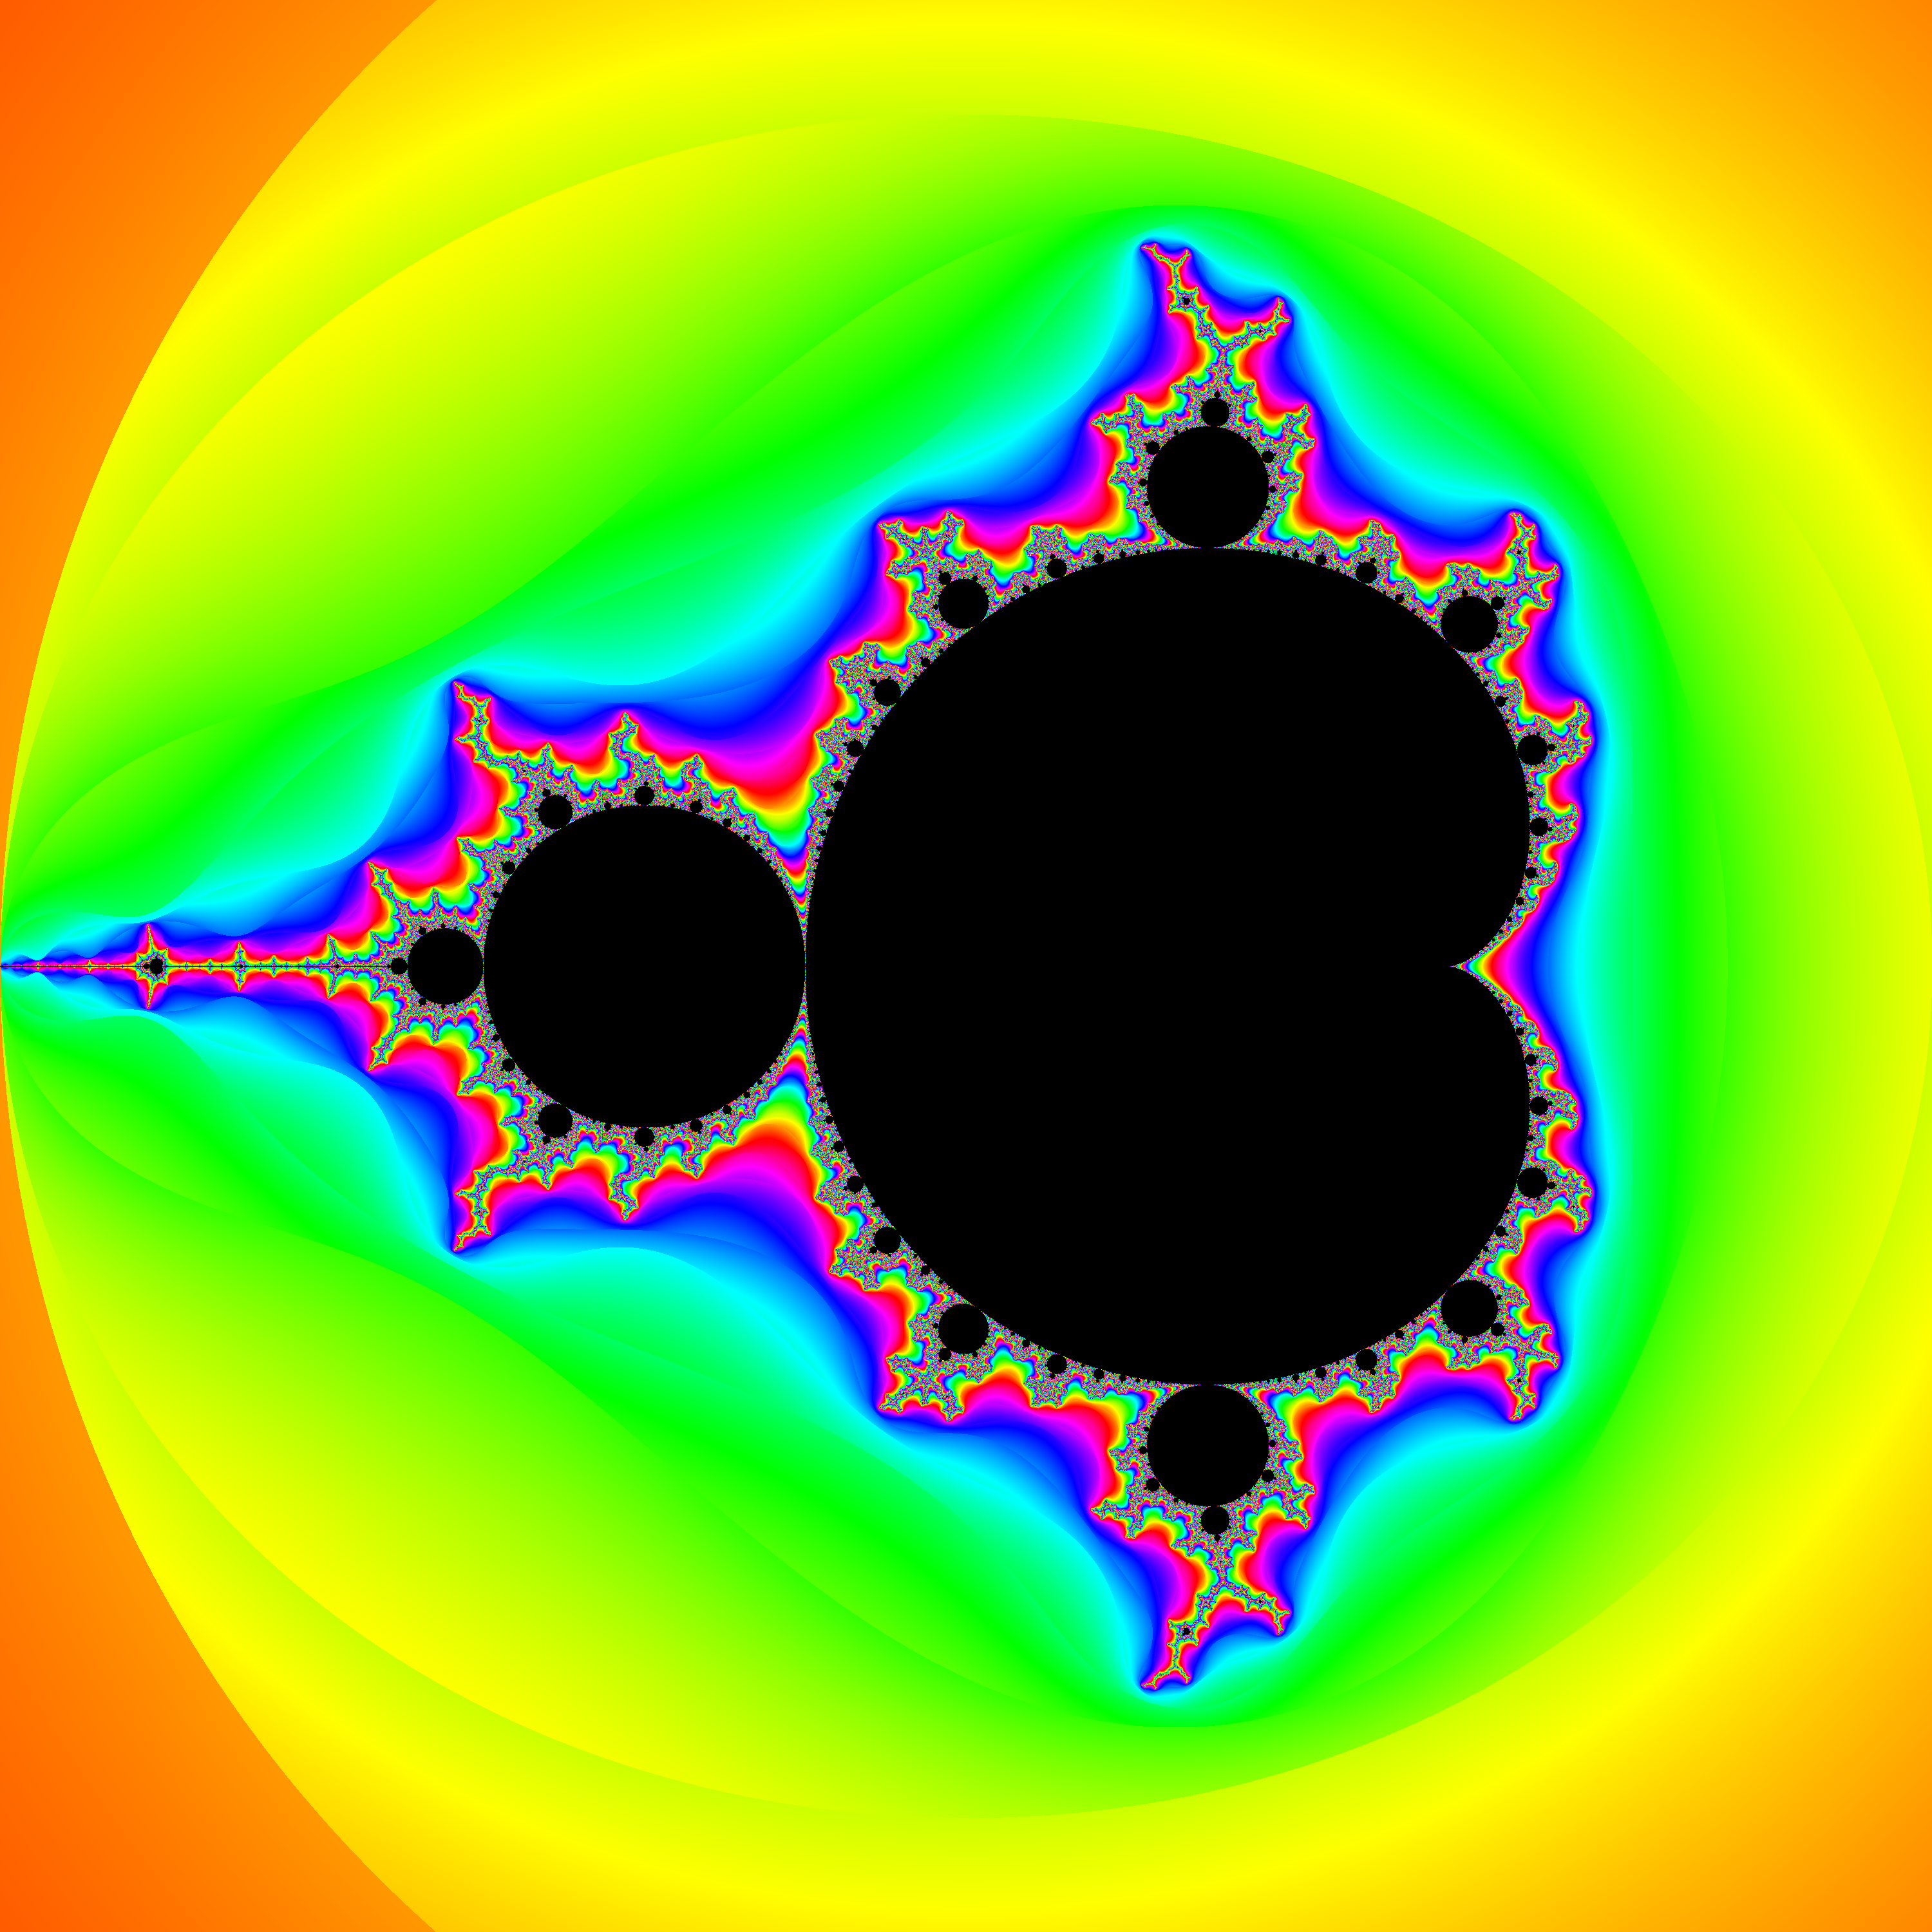
\includegraphics[width=0.95\textwidth]{gfx/figures/mandelbrot.png}
  \caption{Mandelbrot Set (Generated with Code in \autoref{app:code:mandelbrot1})}
  \label{fig:methodology:mandelbrot}
\end{figure}
~\\
To determine if a complex number $c$ is part of the Mandelbrot set, $c$ is applied to the function (\ref{equ:mandelbrot}) with $z_{0}=0$.
\begin{equation}
  z_{n+1} = z_{n}^2 + c
  \label{equ:mandelbrot}
\end{equation}
If the value of $z_{n+1}$ does not diverge over $n$ iterations, $c$ belongs to the Mandelbrot set. In \autoref{fig:methodology:mandelbrot}, all complex numbers $c$, for wich $z_{n+1}$ remains bounded over $n$ iterations are colored black. All other $c$ are colored based on the number of iterations required for $z_{n+1}$ to diverge, with the color spectrum ranging from red (low iteration count) over to blue (high iteration count) indicating increasing iteration counts.

The calculation and visualization of the Mandelbrot set can be partitioned into multiple tasks. Each task executes the same source code but with different input parameters, which define a unique two-dimensional area in the complex plane. These tasks can be executed in parallel due to the independence of calculations between different areas. The implementation for this benchmark is provided in \autoref{ch:appendix}. The source code for the native Go variant can be found in \autoref{app:code:mandelbrot1} and its Go-to-WebAssembly counterpart in \autoref{app:code:mandelbrot2}.
\chapter{Implementation}
\label{ch:implementation}
This chapter presents the technical implementation of the dynamic and heterogeneous volunteer computing platform WebArgo in detail. The implementation leverages modern web technologies introduced in \autoref{sec:methodology:technologies} to create a high-performance distributed computing solution for the web. At its core, the system utilizes WebAssembly for cross-platform compatibility, high-performance, and language independence (\autoref{sec:methodology:wasm}), WebSockets for efficient bidirectional communication (\autoref{sec:methodology:websockets}) and WebWorkers to enhance user experience and to enable potential parallel Task execution (\autoref{sec:methodology:webworker}).

The following sections describe WebArgo's communication protocol, persistence mechanisms, scheduling strategies, security measures and the challenges encountered during the implementation process. \autoref{sec:implementation:backend} and \autoref{sec:implementation:frontend} describe the implementation and usage of WebArgo's \ac{API} and web application interface.

\section{WebArgo's Communication Protocol}
\label{sec:implementation:communication}
When workers or administrators establish a connection to the platform by accessing the frontend application, a WebSocket connection to the backend is automatically initiated. This enables real-time and bidirectional communication between the backend and these clients. Therefore, this connection is used to send tasks from the backend to the workers as well to send the result of each task from the workers back to the backend. Furthermore, administrators receive real-time data about all connected workers and the current status of each job through their WebSocket connection.
\begin{figure}[htbp]
    \centering
    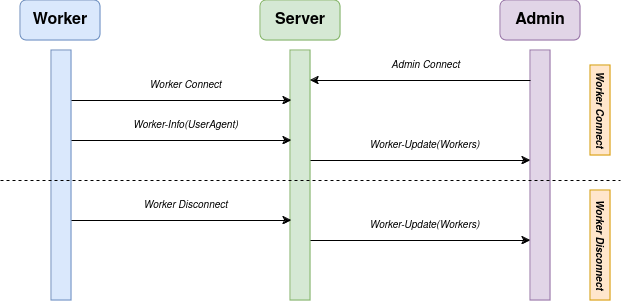
\includegraphics[width=0.9\textwidth]{gfx/figures/communication-connection-label.png}
    \caption{Communication: Connection of Worker \& Real-time Update for Administrator}
    \label{fig:implementation:communication1}
\end{figure}
~\\
The first sequence in \autoref{fig:implementation:communication1} illustrates the process of a worker establishing a connecting to the backend in WebArgo. Upon successful connection, the worker transmits all available information regarding its hardware and operating system in form of the browser user agent to the backend. After this initialization of the worker, all previously connected administrators automatically receive an updated list of all connected workers. Similarly, if a Worker disconnects a automatic update is send to all administrators, as described by the second sequence in \autoref{fig:implementation:communication1}.
\begin{figure}[htbp]
    \centering
    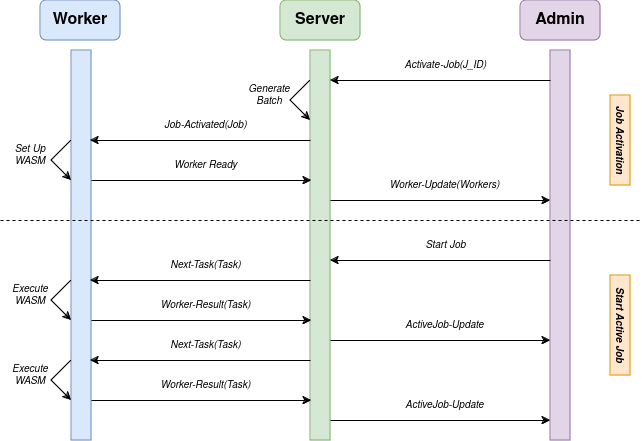
\includegraphics[width=0.95\textwidth]{gfx/figures/communication-jobexecution-label.png}
    \caption{Communication: Administrator Starts Job \& Worker Executes Tasks}
    \label{fig:implementation:communication2}
\end{figure}
~\\
\autoref{fig:implementation:communication2} illustrates the job initialization and execution process. The first sequence describes the job activation process and is initiated when an administrator changes a jobs status to \emph{ACTIVE}. The backend then generates a batch of tasks for this specific job and notifies all connected workers by transmitting a object of this activated job to them. Upon receiving this notification, each worker fetches the corresponding WebAssembly binary and JavaScript glue code file from the backend via \acs{HTTP} request to initializes a WebWorker with the specific WebAssembly environment for this currently active job. When this step is successfully completed the worker notifies the backend, which then marks this workers as \emph{ready}. This update is also forwarded to all administrators with an active WebSocket connection to the backend.

The second sequence in \autoref{fig:implementation:communication2} illustrates th process of starting an active job. This process is initiated when an administrator changes the status of an active job to \emph{RUNNING}. After that begins the backend to distribute unique tasks from the current batch to all workers who have been marked as \emph{ready} by transmitting the \emph{Worker Ready} message and therefore already have successfully completed the initialization process of the currently active job. Each worker executes its assigned task, then appends the corresponding result to the task object and transmits the completed task back to the backend application. If unprocessed or unscheduled tasks remain in the batch at the moment of receiving the completed task, the backend responds by assigning the next pending task to this worker. Additionally, the backend notifies all administrators after each successfully completed task about the current progress of the \emph{RUNNING} job. This enables monitoring of the jobs progression in real-time for all administrators.

If a Worker is connecting to WebArgo while there is already an active or running job, the communication sequence is automatically executed identically. Accordingly, the worker starts to initialize this job and then proceeds to process tasks of the corresponding batch, hence enabling dynamic participation in ongoing jobs for workers.
\\~\\
Each job has a timeout attribute for its tasks. Scheduled tasks that remain incomplete after their allocated timeout period can be redistributed to a different worker. This mechanism enables the rescheduling of tasks, which have been assigned to a malfunctioning worker or a worker that has disconnected before completing its assigned task. Additionally, this approach allows rescheduling of tasks that have been assigned to slower workers, known as stragglers, to more efficient workers. Hence, this mechanism can optimize the overall execution time of a job.
\begin{figure}[htbp]
    \centering
    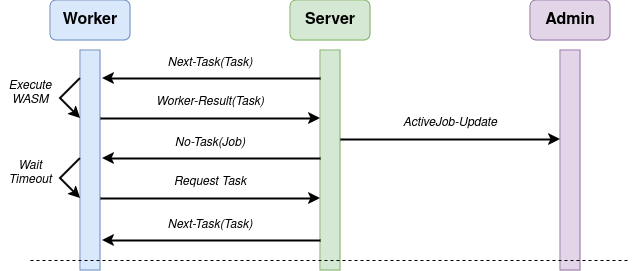
\includegraphics[width=0.95\textwidth]{gfx/figures/communication-timeout.png}
    \caption{Communication: Rescheduling of Tasks after Timeout}
    \label{fig:implementation:communication3}
\end{figure}
~\\
\autoref{fig:implementation:communication3} illustrates the case, if all tasks of the batch already have been scheduled, but one or more are not yet completed. When a worker transmits a completed task to the backend - and therby is expecting to receive a new task to compute from the backend - while the timeout period of all other scheduled tasks has not expired, the backend responds with the \emph{No-Task} message accompanied by the job object of the currently active job. The worker extracts the status and the timeout value from this job objects and initiates a waiting period equivalent to the timeout value plus a randomized overhead, if the jobs status is still \emph{RUNNING}. This additional randomized overhead time prevents simultaneous task requests, if multiple workers are waiting for a task at the same time. After the completion of the waiting period, the worker transmits a \emph{Request Task} message to the backend. The backend responds either with a newly available task or another \emph{No-Task} message, repeating this sequence until the current batch is fully processed.

\section{Persistence}
\label{sec:implementation:persistence}
This section describes the persistent data storage implementation of the platform. The primary adressed objective is to ensure system recovery capabilities in cases of system failures, unexpected system crashes, or scheduled system restarts. The following data objects have been identified as critical for a system recovery:
\begin{itemize}
    \item Job data
    \item Task input arguments
    \item Task results
    \item User credentials
\end{itemize}
Information regarding workers, their hardware specifications and operating systems is intentionally excluded from permanent storage.
\\~\\
WebArgo implements a robust persistence mechanism for job progression. When a running job is stopped, the current progress and all task results are automatically saved, hence actively stopping a running job initiates the persistence process for this job's current state. This functionality should be utilized if the platform is scheduled to be restarted or terminated.

Additionally, the system persists the progress of a currently running job after each batch completion. This mechanism enables periodic job backups, as each batch completion establishes a save point. Consequently, the batch size determines the job's fallback tolerance in the event of an unexpected system failure.

It is noteworthy that from a worker's perspective, task progress can not be persisted. Since WebAssembly is executed in a save sandbox environment the code has usually no access to local files. In the event of an unexpected crash of the worker's WebAssembly process or browser, the progress of the affected task has not been persisted on the workers device and therefore will be lost.

\subsection{Data in Files}
The system utilizes text files for persistent storage of task input arguments and task results. Each job's critical information about its tasks is stored in a separate text file for task input arguments and the task results on the web server. 
~\\
The method to generate a new batch of the active job reads the corresponding task input arguments text file line by line, where each line represents an input argument. For each line, the method creates a unique task and adds it in sequence to the batch.

When the progress of a job is persisted, the backend writes the results of all completed tasks within the batch to the corresponding task results text file. Each result is written in a new line, and the results are stored in sequential order.
\\~\\
Additionally, the backend implements a special mechanism to handle tasks that produce files as results. When a worker transmits such a completed task, the backend immediately stores the result file in a result directory corresponding to the running job. Subsequently, when later a jobs progress is saved, the backend stores the file path to each result in the corresponding task results text file instead of the actual result data.

\subsection{Database}
The PostgreSQL \cite{methodology:db} database is used to store the user credentials as well as each job object. Each job object contains a progress attribute that represents a pointer indexing the last completed task in the task sequence. During job recovery, this progress value determines the starting point for the first task in the new batch.

Furthermore, the following subsections describe the implementation of all entities that are used in WebArgo, as introduced in \autoref{sec:concept:terminology}.

\subsubsection{Job}
The job entity represents a problem to be processed or solved using the WebArgo platform. The platform is designed to handle multiple jobs while each job is a unique object. The State of a job can have one of the following values:
\begin{itemize}
  \item PENDING
  \item ACTIVE
  \item RUNNING
  \item STOPPED
  \item DONE
\end{itemize}
~\\
However, at the current state of the WebArgo implementation only one job at a time can have the \emph{ACTIVE} or \emph{RUNNING} state.

\autoref{fig:methodology:job-task} illustrates the \ac{UML} class diagram for the job entity on the left side, lisitng all important attributes and methods of a job. The language attribute defines the programming langugae of the source code that has been compiled to a WebAssembly binary file.
\\~\\
Job entities are stored on the database and can be loaded from the backend. Additionally, the backend provides a compromised \ac{DTO} of each job object for workers or administrator users.
\begin{figure}[htbp]
    \centering
    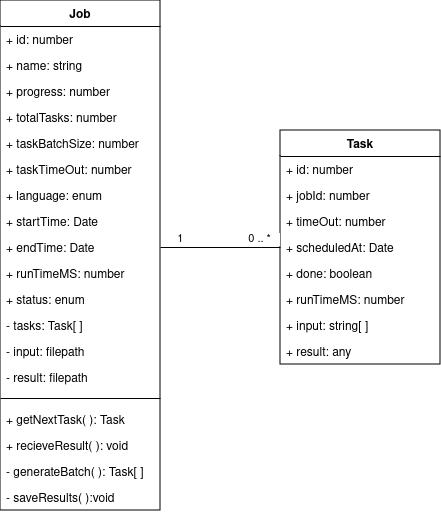
\includegraphics[width=0.75\textwidth]{gfx/figures/Job-Task.png}
    \caption{\acs{UML} Class Diagram: Job \& Task}
    \label{fig:methodology:job-task}
\end{figure}

\subsubsection{Task}
Each job is divided into multiple tasks and ideally has each task an equal computational workload. These tasks are distributed to the participating worker nodes. Tasks are unique objects, each holding the specific input parameters that describe the particular portion of the job to which the task is assigned. \autoref{fig:methodology:job-task} displays the \ac{UML} class diagram for the task entity on the right side. The relationship between the job and task entities is defined as One-to-Many, meaning a job can consist of multiple tasks, but each task is always assigned to a single job.

A batch is defined to be a subset of tasks, which are all assigned to the same job. When the state of a job becomes \emph{ACTIVE} the backend enriches the \emph{tasks} attribute of this job object to match the current batch of this job.
\\~\\
Tasks are not stored in the database, but dynamically generated in the backend under utilization of the corresponding task input argument file stored on the web server. These tasks are then distributed to workers for computation.

\subsubsection{User}
A user represents a client that accesses the WebArgo platform through the frontend application. The actions a user can perform are determined by its assigned user role. This user role can either have the value \emph{User} for limited access or \emph{Admin} for full access to all features. \autoref{fig:methodology:client} displays the \ac{UML} class diagram for the user entity at the top of the illustration. This user information is stored in the database and used for the security measures, later described in \autoref{sec:implementation:authentication}. 

\begin{figure}[htbp]
    \centering
    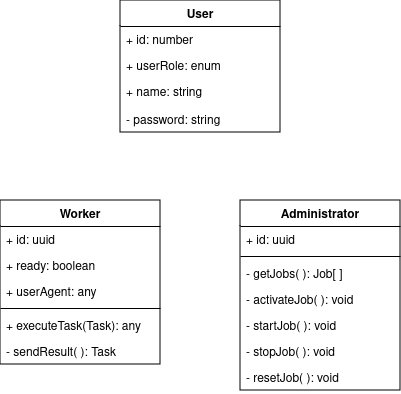
\includegraphics[width=0.75\textwidth]{gfx/figures/Client.png}
    \caption{\acs{UML} Class Diagram: User | Worker \& Administrator}
    \label{fig:methodology:client}
\end{figure}
~\\
Workers receive tasks from the current batch of the active job, compute these tasks, and send the corresponding results to the backend. \autoref{fig:methodology:client} presents the \ac{UML} class diagram of the worker entity on the left side, listing all relevant attributes and methods. As workers connect to the frontend via web browsers, the browser's user agent is utilized to individually characterize each worker. This so-called browser user agent can be accessed inside the clients browser environment and provides information about the client's hardware resources and operating system. A worker object is dynamically generated in the frontend and backend application when a worker client accesses WebArgo.
\\~\\
An administrator user can perform the same actions as a worker, but also has additional capabilities. Only administrators have the ability to set or change the state of jobs and to oversee the progress of all jobs. \autoref{fig:methodology:client} illustrates the \ac{UML} class diagram of the administrator entity on the right side. When an administrator accesses the WebArgo platform an corresponding administrator object is dynamically generated in the frontend and backend application.

\section{Scheduling}
\label{sec:implementation:scheduling}
The backend is responsible for distributing tasks from the current batch to participating workers. To maximize performance, the backend keeps track of scheduled tasks to prevent duplicate task distribution among workers. The scheduling of tasks follows the \ac{FIFO} methodology, scheduling the tasks in sequential order. As described in \autoref{sec:implementation:communication}, each job object has a timeout attribute for its tasks. Only if a task remains incomplete after its designated timeout period has expired, can this task be rescheduled. This mechanism serves to mitigate issues that arise from malfunctioning, disconnected, or straggling workers.
\\~\\
The scheduling mechanism could be enhanced through the implementation of performance-aware distribution, allocating computationally intensive tasks to workers identified to possess superior hardware. Furthermore, these identified stronger workers could execute multiple WebWorker with different tasks, performing parallel task execution on a single worker instance.

\section{Security through Authentication \& Authorization}
\label{sec:implementation:authentication}
To prevent malicious use, particularly in critical processes managed by administrators, the system implements a authentication mechanism. This is achieved through user credentials combined with a \ac{JWT}.

Authentication and Authorization are two key security concepts that work together to protect systems and data. Authentication is used to verify a clients identity - proving they are who they claim to be - in this platform realized through user credentials. Once a user is authenticated, Authorization determines what they're allowed to do within the system by checking their permissions and access rights. The \emph{userRole} attribute in the user object defines the specific access permissions. Together, these processes ensure that users are verified and these authenticated users can only access the resources and perform the actions appropriate for their role or permission level.

A \ac{JWT} implements a compact, \acs{URL}-safe methodology for secure information transmission between parties as a \ac{JSON} object \cite{implementation:jwt}. The token architecture comprises three dot-separated components: a header that describes the token type and signing algorithm, a payload containing the encoded data and a signature to verify the token's authenticity \cite{implementation:jwt}. \ac{JWT}s are commonly used in authentication and authorization processes, where information like user identity and permissions needs to be securely shared between services. The token can be verified by other services using the signature, eliminating the need to repeatedly validate credentials against a database. This makes \ac{JWT}s particularly useful in modern web applications and microservices architectures where secure, stateless authentication is required. \cite{implementation:jwt}

Upon successful user authentication, when a client connects to the platform, the backend generates and sings a \ac{JWT}, which is used to authenticate subsequent requests of this user. This generated \ac{JWT} is stored as a browser cookie on the client side which remains valid during a two-day expiration period. The data stored in the \ac{JWT} payload is a \ac{JSON} object containing the attributes \emph{id}, \emph{name}, and \emph{userRole} corresponding to the authenticated user. Clients transmit their specific \ac{JWT} with every \ac{API} request or when establishing a WebSocket connection. Hence, the backend can then use this token to authenticate the user and check if the user is authorized for this action.

\section{Backend}
\label{sec:implementation:backend}
This section describes the usage and features of the backend, which is implemented using the NestJS \cite{methodology:nestjs} framework. The backend application serves three primary functions: 
\begin{itemize}
    \item Data management for users, jobs, tasks, and their associated results.
    \item Handling the WebSockets communication with all connected clients.
    \item Task distribution to participating workers.
\end{itemize}
~\\
To manage and interact with jobs or users, the backend exposes multiple endpoints through a \acs{REST}ful \ac{API}. \autoref{fig:implementation:backend} presents a list of all available endpoints and their corresponding \acs{HTTP} request method. Due to their handling of critical and sensitive data, all endpoints are secured through \ac{JWT} authorization and always require administrator privileges, granted only for users with the \emph{Admin} \emph{userRole}. The login endpoint represents the only exception to this security measure, as it serves to generate a \ac{JWT} in the first place by validating a users credentials, and therefore operates without any \ac{JWT} authorization.

The backend \ac{API} implements comprehensive \ac{CRUD} operations for both job and user entities. These endpoints enable the retrieval of individual objects or complete object collections, the creation of new objects, and the modification or removal of existing objects. Furthermore, the \ac{API} exposes four additional endpoints to change the state of jobs and therefore providing the features to control job execution of WebArgo. Upon job activation, a batch associated to this job is generated and all connected workers are triggered to initiate the initialization of their corresponding WebAssembly environment. Starting a job initiates the process of distributing tasks from its batch to \emph{ready} participating workers. When a job is stopped, its current state is persisted on the web server as described in \autoref{sec:implementation:persistence}. The job reset operation permanently removes all progress associated with a job and generates a new unprocessed batch containing the initial tasks.
\begin{figure}[bth]
    \myfloatalign
    \subfloat[Job \ac{API} endpoints]{
    \label{fig:implementation:backend:job}
    
\includegraphics[width=.25\linewidth]{gfx/figures/Job_API.png}
    } \quad \quad
    \subfloat[User \ac{API} endpoints]{
    \label{fig:implementation:backend:user}
    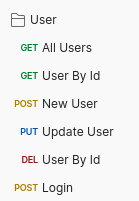
\includegraphics[width=.25\linewidth]{gfx/figures/User_API.png}
    }
    \caption{Available Backend \ac{API} endpoints}
    \label{fig:implementation:backend}
\end{figure}
~\\
Additionally, the backend \ac{API} serves static files of the compiled WebAssembly binaries and the optional required JavaScript glue code files for each job. These files are required to initializes a WebAssembly environment, and are therefore requested by worker nodes.

Furthermore, the backend implements the WebSocket-based communication protocol as described in \autoref{sec:implementation:communication} that manages bidirectional data streams between the backend and connected clients. This implementation enables performant task distribution and task result collection as well as real-time comunication for job progress monitoring while minimizing the overall communication overhead.

\section{Frontend}
\label{sec:implementation:frontend}
This section describes the features and main web pages served by the frontend. It is implemented utilizing the NextJS \cite{methodology:nextjs} framework in combination with styled components from the React Bootstrap library \cite{implementation:bootstrap}. The core features implemented in the frontend application are:
\begin{itemize}
    \item Providing an easy to use interface to interact with WebArgo
    \item Establishing a WebSocket connection between clients and the backend
    \item Computing tasks with WebAssembly in a WebWorker
    \item Serving a dashboard for administrators to manage jobs
\end{itemize}
The frontend implements two main web pages. These are the \emph{Dashboard Page} and the \emph{Client Page}.

\subsection{Dashboard Page}
\label{subsec:implementation:dashboard-page}
The \emph{Dashboard Page}, displayed in \autoref{fig:implementation:dashboard-page}, is only accessible for administrators. This page is used to monitor all connected workers and the progress of jobs in real-time. Furthermore, are administrators able to manage jobs through this web page.
\begin{figure}[htbp]
    \myfloatalign
    \subfloat[Dashboard Page: Job List]{
        \label{fig:implementation:job-list}
        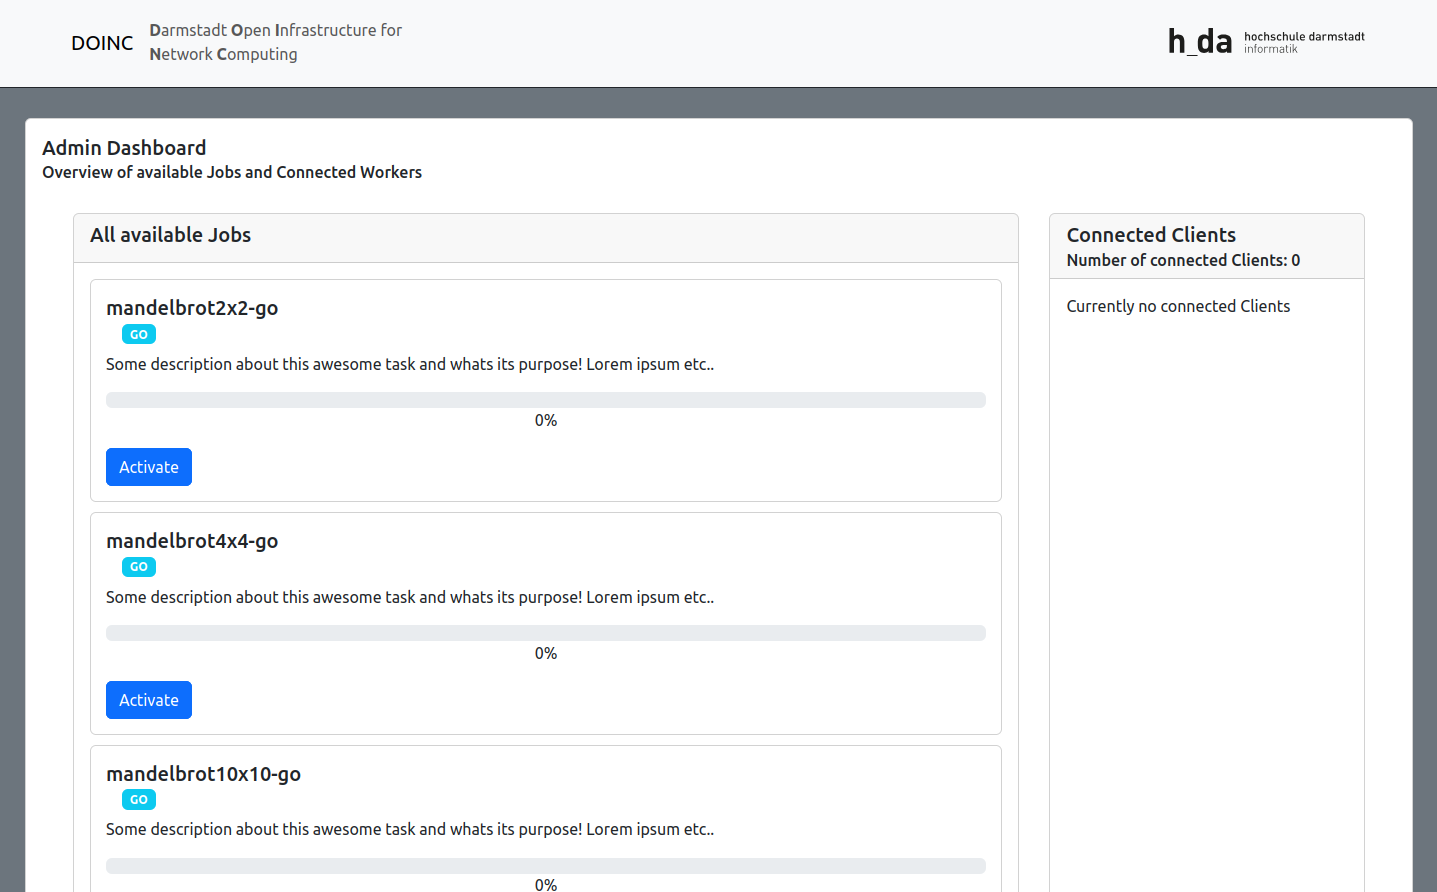
\includegraphics[width=.8\textwidth]{gfx/figures/job-list.png}
    } \\
    \subfloat[Dashboard Page: Active Job]{
        \label{fig:implementation:active-job}
        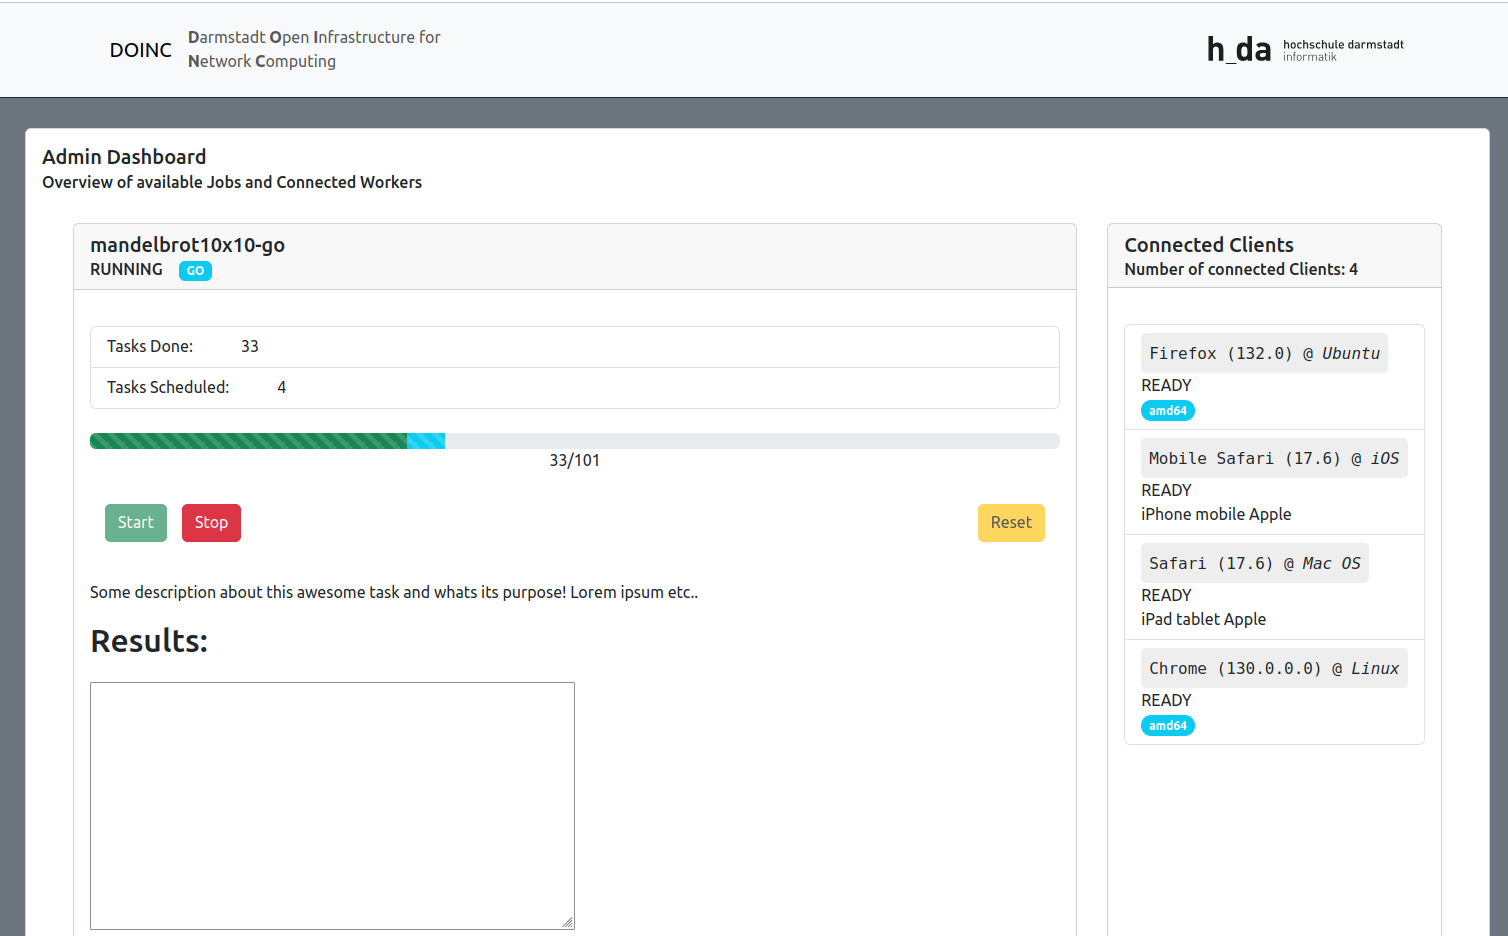
\includegraphics[width=.8\linewidth]{gfx/figures/active-job-2.png}
    }
    \caption{Frontend Dashboard Page}
    \label{fig:implementation:dashboard-page}
\end{figure}
~\\
On the left side of the \emph{Dashboard Page} is a component located to manage the jobs of the platform. It holds a list of all existing jobs and their current progress, displayed in \autoref{fig:implementation:job-list}. Above this list of jobs appears a new component when a job is activated by an administrator.

\autoref{fig:implementation:active-job} displays a view of this active job component on the left side. This component visualizes the progress of an active job and displays the gathered results of complete tasks after each batch completion in real-time. Additionally it provides an interface to interact with this job. When a button of this interface is clicked, a corresponding \acs{HTTP} request, containing the administrator's \ac{JWT}, is transmitted to the backend. After all tasks are completed and the state of the job is \emph{DONE}, this component presents information about the total run time of the job. 

On the right side is another component located that displays a list of all connected workers, also in real-time. This list contains information about the initialization progress as well as the hardware and operating system for each worker with an active WebSocket connection to the backend. A view of this list is displayed in \autoref{fig:implementation:active-job} on the right side.

\subsection{Client Page}
\label{subsec:implementation:client-page}
The \emph{Client Page} represents the logic for workers and can be accessed by workers or administrators. When a client is accessing this web page the browser process becomes a participating worker in the WebArgo volunteer computing platform. First the worker establishes a WebSocket connection to the backend to receive job and task data and to send task results as described in \autoref{sec:implementation:communication}. If this connection is successful the browser user agent of the workers device is extracted and transmitted to the backend. When a job is active or running the connected worker is creating an independent browser thread - the WebWorker - and initializes the corresponding WebAssembly environment inside this WebWorker. Each task that the worker is receiving is forwarded for computation to this WebWorker. The performance and availability of the main browser thread, responsible for the \ac{UI} and WebSocket connection, is not affected by the processing of incoming tasks, since the intensive WebAssembly computation is handled inside the separate and independent WebWorker.

\autoref{fig:implementation:client-page} displays the view of the \emph{Client Page}. The main component of this page presents various information about the worker, like the status of its WebSocket connection, the current actively supported job and statistics about all tasks that have been completed by this worker. Therefore workers can always monitor the current status of their device, task computation and what kind of job they are supporting. Additionally, the usage of a WebWorker for the WebAssembly execution prevents the user page from becoming unresponsive or frozen during task computation. This enhances the user experience and also is supposed to prevent workers from potentially disconnecting because they could experience a unexpected frozen \ac{UI}.
\clearpage
\begin{figure}[htbp]
    \centering
    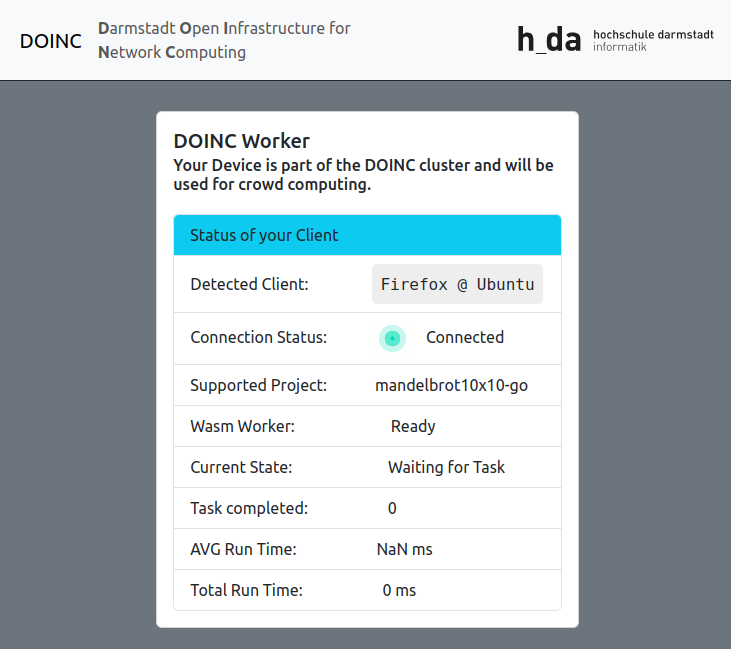
\includegraphics[width=0.8\textwidth]{gfx/figures/client-page.png}
    \caption{Frontend Client Page}
    \label{fig:implementation:client-page}
\end{figure}
~\\
In the current state of WebArgo the worker is implemented to initialize and execute WebAssembly binaries complied from either C \& C++, Go or Python source code. The support of further WebAssembly targeting languages can be added effortlessly to this work, since the usage of WebWorker scripts is handled generic. To support specific programming languages each WebWorker script requires additional unique glue code during the WebAssembly initialization process.

\section{Benchmark}
\label{sec:implementation:benchmark}
As described in \autoref{sec:methodology:benchmark}, the visualization of the Mandelbrot set is used to benchmark the performance of the volunteer computing platform in \autoref{ch:evaluation}. To achieve this, this job is distributed among multiple workers through the WebArgo platform and the resulting total execution time of this approach is then compared to the total execution time of the same job on a single device in a native environment.

Since the Mandelbrot set represents a subset of complex numbers, it is visualized in a two-dimensional coordinate system representing the two-dimensional complex plane. The primary region of interest is located in an area bounded by $1$ to $-2$ on the X-axis (real numbers) and $1.5$ to $-1.5$ on the Y-axis (imaginary numbers). This area is partitioned into 100 equally sized sections, forming a 10x10 grid. \autoref{fig:implementation:mandelbrot-page} visualizes the Mandelbrot set's primary region of interest divided into 100 equal areas.
\clearpage 
\begin{figure}[htbp]
    \centering
    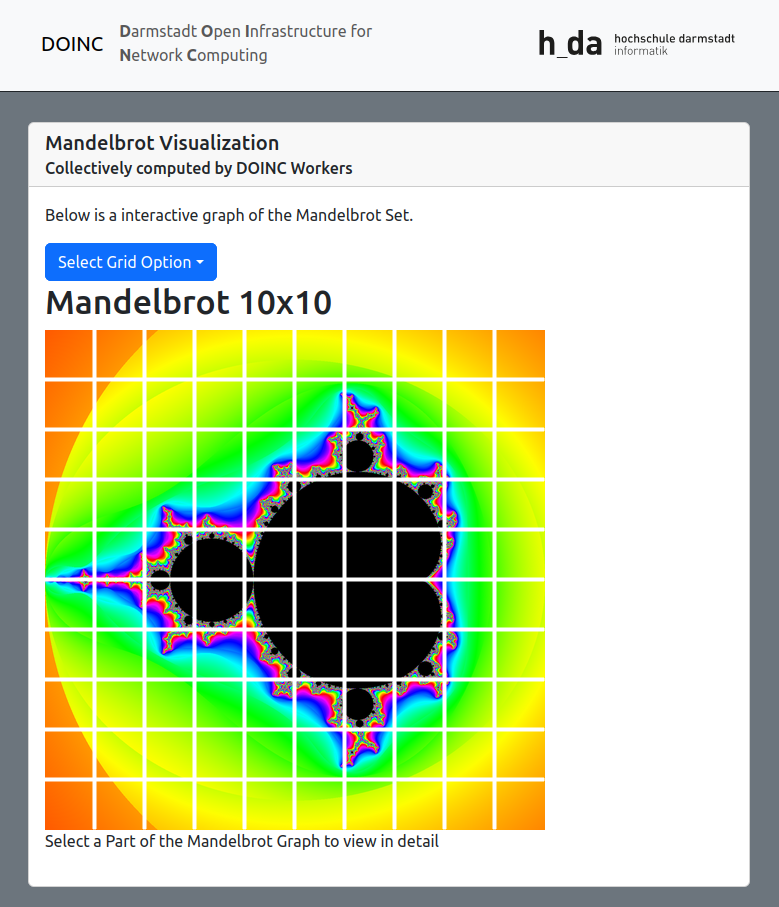
\includegraphics[width=0.95\textwidth]{gfx/figures/mandelbrot-page.png}
    \caption{Frontend Mandelbrot Page}
    \label{fig:implementation:mandelbrot-page}
\end{figure}
~\\
Each grid tile represents the input arguments of a distinct task. An additional task computes the entire area of the Mandelbrot set at a lower resolution as a thumbnail, resulting in a total of 101 unique tasks for the benchmark job. Each of these tasks is generating a \acs{PNG} file that visualizes the corresponding Mandelbrot set tile, utilizing the same color scheme as illustrated in \autoref{fig:methodology:mandelbrot}. Each task computes the Mandelbrot condition for 2.25 million complex numbers $c$ within a 1500x1500 square region. Each of these 2.25 million $c$ represents a pixel in the \acs{PNG} file generated by the task. On task completion the generated \acs{PNG} file is transmitted to the backend through the WebSocket connection and stored on the web server in a corresponding directory. After the job is successfully completed an interactive visualization of the Mandelbrot set becomes accessible via the \emph{Mandelbrot page}, served by the frontend application. This specific page is displayed in \autoref{fig:implementation:mandelbrot-page}. Each tile and the thumbnail picture is computed and generated by a worker, representing the workload of a single task. By clicking on one of these tiles on the thumbnail, the corresponding \acs{PNG} picture can be viewed in its original resolution underneath the interactive Mandelbrot visualization component.

The WebAssembly-compatible Go source code, which is executed by workers during Task computation, is presented in \autoref{app:code:mandelbrot2}. The corresponding native Go implementation, executed in comparision on a single device, can be found in \autoref{app:code:mandelbrot3}.

\section{Challenges}
\label{sec:implementation:challenges}
This section lists and describes the  challenges that occurred during the development process of the volunteer computing platform.
\newline
\newline
\textbf{Generic implementation of Jobs:}
\newline
The platform is designed to allow the execution of any kind of custom job. To ensure a flexible development of new jobs, the job entity and the handling of tasks, WebAssembly binaries, and input arguments are implemented using generic patterns throughout the architecture in all components. This enables the distribution of jobs across the platform, written in any supported programming language and with any amount of tasks, effortlessly with a minimal programming overhead.
\newline
\newline
\textbf{Loading glue code and WebAssembly files from external source (Backend) inside WebWorker:}
\newline
To maintain simplicity, all WebAssembly binaries and their associated glue code files are centrally stored in their corresponding job directory on the web server, hence ensuring that all files specific to a job remain in a single location. However, the initialization of the WebAssembly environment in the \emph{Client Page} of the frontend requires fetching and incorporating files from the backend as a third-party source in this design. This behavior presented a challenge during the implementation, as the glue code scripts expect its corresponding WebAssembly binary to be located in the same local directory instead of being externaly loaded. It was not trivial to reproduce this behavior inside the WebWorker.
\newline
\newline
\textbf{Handling the Input and Output of WebAssembly code:}
\newline
A string array format, similar to conventional command-line input arguments, has been selected as the uniform input type across all tasks. This standardized format enables simple parsing of arguments from the input text files and can also be effortlessly forwarded to WebAssembly functions within the JavaScript runtime environment.

The implementation of a generic output format across all tasks and programming languages presented significant challenges. Especially for C and C++ source code, where the \emph{main} function is constrained to return always a single numeric value (\emph{int}). However, the developed solution supports the output of any primitive datatypes, lists of primitive datatypes, objects and also binaries, even for C and C++ applications. This behaviour applies to all kinds of tasks throughout all supported programming languages.

To enable binaries as task output the WebSocket connection between workers and the backend had to be adjusted. The default message size limit (\emph{maxHttpBufferSize}) of the Socket.IO \cite{methodology:websockets2} library has been raised to $100MB$ per message to ensure the transmission of larger files.
\newline
\newline
\textbf{Implement system recovery measures:}
\newline
The design and implementation of system recovery mechanisms, as described in \autoref{sec:implementation:persistence}, has represented a complex enhancement to the platform.
\newline
\newline
\textbf{Prevent duplicate Task execution \& ensure Job completion in case of malfunctioning Workers:}
\newline
The timeout mechanism described in \autoref{sec:implementation:scheduling}, comparable but not identical to the timeout implementation of XtremWeb \cite{relatedwork:xtremweb}, was a crucial enhancement that had to be integrated into the scheduling process. This timeout mechanism is used to prevent duplicate task execution and ensures rescheduling of aborted tasks.
\chapter{Evaluation}
\label{ch:evaluation}
This chapter presents the evaluation of the implemented WebCrowd platform through a series of experiments designed to address the research questions defined in \autoref{subsec:into:objectives:questions}. These three research questions focus on WebCrowds computational capabilities when handling complex parallelizable tasks, its dynamic viability in managing fluctuating worker participation, and its ability to support heterogeneous devices as workers. Each of the following sections in this chapter corresponds to one of the research questions and presents the experimental setup, the expected outcome, and a analysis of these results.

The experiments of the evaluation utilize the implemented visualization of the Mandelbrot set, described in \autoref{sec:implementation:benchmark}, as a benchmark job. This benchmark job represents a computationally intensive test case, which can be used to demonstrate and test WebCrowd's capabilities. Each task of this benchmark job coveres a unique 1500x1500 area of the Mandelbrot set and all generated \ac{PNG} files have the same resolution. However, the computation time varies significantly among each of these tasks. According to the Mandelbrot function in (\ref{equ:mandelbrot}) require complex numberers that are part of the Mandelbrot set more iterations of the calculation than complex numbers that are not part of the Mandelbrot set. Therefore depends the execution time of a task on the amount of calculated points that belong to the Mandelbrot set.

Additionally, \autoref{sec:evaluation:languages} compares the performance of the various in WebCrowd implemented WebAssembly environments, each supporting the execution of source code from different programming languages compiled to a WebAssembly binary.

\section{Computational Capability}
\label{sec:evaluation:computation}
\textbf{Is WebCrowd capable of successfully solving large, parallelizable problems?} 
\newline
The objective of the following experiment is to evaluate WebCrowd's ability to successfully execute computationally intensive, parallelizable tasks across a distributed network of volunteer workers. This empirical experiment compares the total execution time between distributed computation across multiple workers and native execution on a single computer.

\subsection{Experimental Setup}
The batch size of the benchmark job was set to 101. Therfore, only a singel batch is generated and processed during all experiments and the job progress is only persisted once upon completion of all 101 tasks.

At first the benchmark job was computed on the system specified in \autoref{app:system:server} in a native Go environment using the source code of \autoref{app:code:mandelbrot3}. The resulting computation time serves as a baseline for the following experiments, because this system is later also used to host the WebCrowd platform. Since this system is already required to serve WebCrowd in the first place, the following experiments additionally investigate whether distributing the workload to external clients provides a performance advantage compared to utilizing the existing host system for computation. Throughout the experiments, all workers maintained available and executed only the WebCrowd browser process. The benchmark job was evaluated across the following six distinct scenarios:
\begin{itemize}
    \item Two homogeneous and independent smartphones with the harware specified in \autoref{app:system:phone} as workers, executing the client page in a Apple Safari 18.1 \cite{evaluation:safari} browser
    \item Three homogeneous and independent smartphones with the harware specified in \autoref{app:system:phone} as workers, executing the client page in a Apple Safari 18.1 \cite{evaluation:safari} browser
    \item Three parallel Mozilla Firefox 132.0 \cite{background:firefox} browser taps of the client page on a single laptop, specified in \autoref{app:system:mymachine}
    \item Three parallel Microsoft Edge 131.0.0.0 \cite{evaluation:edge} browser taps of the client page on the same \acs{PC}, specified in \autoref{app:system:mypc}
    \item 16 homogeneous and independent single-board computers with the harware specified in \autoref{app:system:pi} as workers, each executing the client page in a headless Mozilla Firefox 133.0 \cite{background:firefox2} browser
    \item 32 homogeneous and independent single-board computers with the harware specified in \autoref{app:system:pi} as workers, each executing the client page in a headless Mozilla Firefox 133.0 \cite{background:firefox2} browser
\end{itemize}

\subsection{Expectations}
It is expected that all tasks of the benchmark job will be scheduled as intended and distributed over all participating workers and each task result is successfully received by the server and saved on the server. To verify if this process was successful, each worker is monitored through the interface of the client page during the experiment and after the experiment is the implemented mandelbrot page (\autoref{sec:implementation:benchmark}) utilized to examine the generated task results.

Additinally, all experiments are carried out using the interactive dashboard page (\autoref{subsec:implementation:dashboard-page}) to start and monitor the execution of the benchmark job. It is expected that all features of this application work as intended and the job progress as well as all participating workers can be monitored in real-time.

Furthermore, based on the theoretical model presented in \autoref{sec:background:theory}, distributing the benchmark job across multiple workers should reduce the total execution time of a job when the number of workers $N$ exceeds the threshold value represented in the inequality term of \eqref{equ:transformation2}. To estimate this threshold value of $N$ for all previously listed experiment scenarios the amount of tasks $T$ was set to 101 and an Internet latency of 32 ms \cite{backend:latency} was assumed for $t_{L}$. Since the computation times $t_{Native}$ and $t_{Virtual}$ are not equal for all 101 tasks, a heavy computational task - handeling the center of the Mandelbrot set - was selected to represent these computation times. This single task has been executed and measured independently on the native Go environment on the server system as well as on the WebAssembly browser environment through the WebCrowd platform for each device participating in the experiment as worker. The computation time $t_{Native}$ of this computationally heavy task was measured to be 34.60 seconds on the server system specified in \autoref{app:system:server}. The corresponding computation time $t_{Virtual}$ of the same task was measured to be 57.53 seconds using the Apple Safari 18.1 \cite{evaluation:safari} browser on a smartphone specified in \autoref{app:system:phone}, 1 minute and 34.8 seconds using the Mozilla Firefox 132.0 \cite{background:firefox} browser on the laptop specified in \autoref{app:system:mymachine}, 1 minute and 28.2 seconds using the Microsoft Edge 131.0.0.0 \cite{evaluation:edge} browser on the \acs{PC} specified in \autoref{app:system:mypc} and a total of 7 minutes and 13.2 seconds using the headless Mozilla Firefox 133.0 \cite{background:firefox2} browser on one single-board computer specified in \autoref{app:system:pi}. With this information the amount of workers $N$ - expected to provide a performance advantage compared to the native code execution - was calculated with the inequality term of \eqref{equ:transformation2} for each scenerio:
\begin{itemize}
    \item \textbf{Smartphones:} $N > 1.7$, meaning two or more smartphones are expected to achieve a performance gain 
    \item \textbf{Laptops:} $N > 2.8$, meaning three or more laptops are expected to achieve a performance gain
    \item \textbf{PCs:} $N > 2.6$, meaning three or more \acs{PC}s are expected to achieve a performance gain
    \item \textbf{Single-board computers:} $N > 14.3$, meaning 15 or more single-board computers are expected to achieve a performance gain
\end{itemize}

\subsection{Results}
The benchmark job was successfully computed in every experiment and all features of the web application behaved as intended.
\newpage
\begin{figure}[htbp]
    \centering
    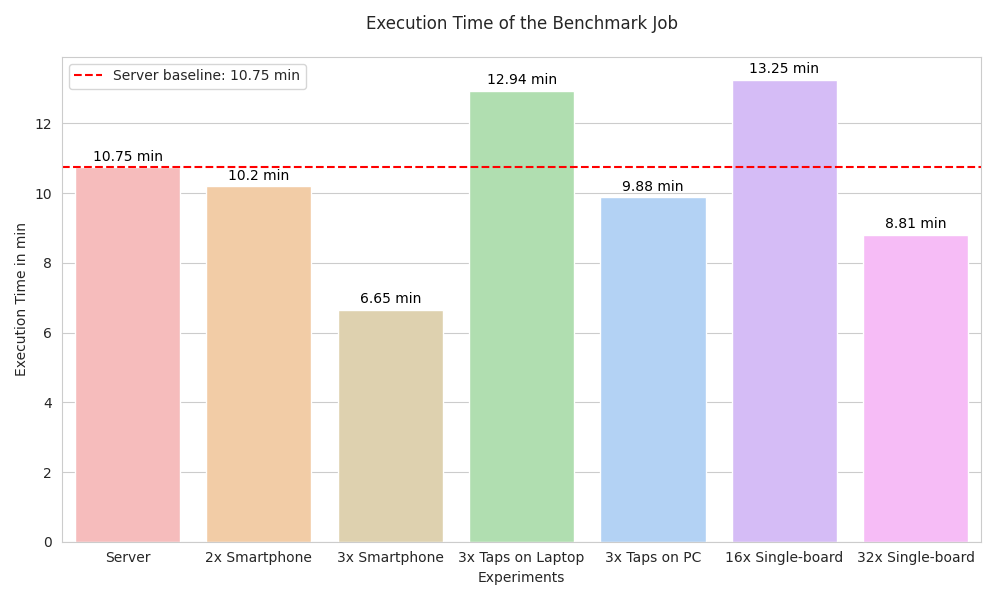
\includegraphics[width=0.95\textwidth]{gfx/figures/Evaluation_A.png}
    \caption{WebCrowd Execution Time Compared to Native Execution Time}
    \label{fig:evaluation:experiment-A}
\end{figure}
~\\
\autoref{fig:evaluation:experiment-A} compares the measured execution times of the different experiments to the baseline time of the server. The native execution on the server system completed all 101 tasks in an average execution time $t_{ExSeq}$ of 10 minutes and 45 seconds across three runs. Distributing the benchmark job across the two smartphone workers resulted in a total execution time $t_{ExDist}$ of 10 minutes and 12 seconds, and therfore faster than the baseline as predicted. With three smartphone workers, the execution time further decreased to 6 minutes and 39 seconds, representing a performance improvement of 38\% compared to the native execution on the server. 

Distributing the benchmark job across three browser taps on the laptop took 12 minutes and 56.4 seconds to complete the total workload. This approach did not achieve a performance gain compared to the native code execution on the server. However, distributing the benchmark job across three browser taps on the \acs{PC} complete the total workload in only 9 minutes and 52.8 seconds and therfore faster than the baseline of the server. These two experiments show that a single device can be successfully utilized to participate in WebCrowd with running multiple worker processes in parallel, and therfore effectively allows to expand the job progress computed by a single device. But it can not be expected that a single browser tab in this scenario will behave in the same way as an independent device. The bahavior of multiple worker tabs on a single device most likely depends on the devices hardware, the amount of available \acs{CPU} cores and the browser and operating system used.

Utilizing the 16 independent single-board computers resulted in a total execution time $t_{ExDist}$ of 13 minutes and 15 seconds, and therfore did not achieve an expected performance gain compared to the native code execution. Since all single-board computers are continuously transmitting \ac{PNG} files across a shared networking hardware, a reason for this unexpected longer total execution time could be congestion, jamming or packet loss in the communication between the single-board computers and the server. Because the WebSocket communication utilized in WebCrowd is leveraging the \ac{TCP}, packet loss does not impact the result of the job, but could increase the overall computation time due to retransmission of network packets. However, the network communication has not been further investigated, therfore it can not be excluded that this unexpected slowdown issue is caused by something else. Distributing the same workload across 32 single-board computers completed the benchamrk job in 8 minutes and 48.6 seconds.
\\~\\
These results overall validate the predictions of the theoretical model presented in \autoref{sec:background:theory}. Furthermore, these experiments demonstrate that WebCrowd can successfully leverage parallel processing through volunteer computing to reduce the total computation time of a job, despite the overhead of communicating through the Internet and the longer computation time $t_{Virtual}$ in the WebAssembly environment. This performance gain scales with the number of participating workers $N$.

\section{Dynamic Viability}
\label{sec:evaluation:dynamic}
\textbf{Is the WebCrowd platform stable in a environment with dynamic clients?}
\newline
The second research question investigates whether WebCrowd maintains stability in an environment with dynamic clients, addressing a fundamental challenge in volunteer computing where worker participation is inherently unpredictable and therfore dynamic. This evaluation is crucial, as a key feature of WebCrowd is to maintain operational despite workers joining or leaving at any time. Hence, the following experiments in this section evaluate WebCrowd's ability to handle fluctuating worker participation.

\subsection{Experimental Setup}
To evaluate WebCrowd's dynamic viability, the platform was tested in a controlled environment with manually connecting or disconnecting workers. The experiments utilized 32 single-board computers specified in \autoref{app:system:pi}, each running a headless Mozilla Firefox 133.0 \cite{background:firefox2} browser to participate in WebCrowd as a worker through the cleint web application. \autoref{evaluation:pilab} further describes the technical setup of these single-board computers. The task timeout to enable rescheduling of aborted tasks was set to be 60 seconds throughout the benchmark job. The following two experiments were conducted to simulate a dynamic environment where workers join or leave the network during the execution of an active job:
\begin{enumerate}
    \item Disconnecting of 8 workers (25\% of all conneted workers) after about 50\% of total job completion 
    \item Starting with 8 connected workers and gradually connecting more devices until 32 workers are connected
\end{enumerate}
Again, the Mandelbrot benchmark job was utilized for these experiments.

\subsubsection{Pi-lab from h\_da}
\label{evaluation:pilab}
TODO

\subsection{Expectations}
It is expected that all 101 tasks of the bechmark job are successfully completed, regardless of the fluctuating behaviour of workers. Hence, aborted task from disconnected workers are expected to be rescheduled to other availabile workers, and workers wich are connecting while the active job is already running are expected to automatically setup the corresponding WebAssembly environment and then immediately participate as workers.

\subsection{Results}
The benchmark job was successfully computed in both experiments and all connecting workers have actively participated in computing the workload of the job. Therfore, these experimental results demonstrate WebCrowd's robust handling of dynamic worker participation. \autoref{fig:evaluation:experiment-B} displays the total computaion time of both experiments compared to the basline computation time of 32 permanently connected single-board computers as workers, previously measured in \autoref{sec:evaluation:computation}.
\begin{figure}[htbp]
    \centering
    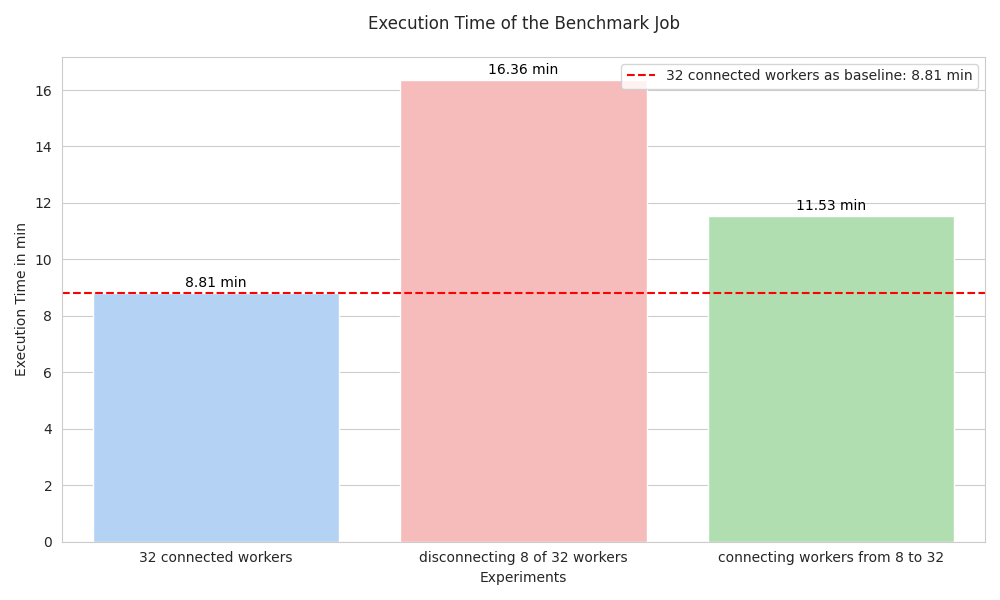
\includegraphics[width=0.95\textwidth]{gfx/figures/Evaluation_B.png}
    \caption{WebCrowd Execution Time in Dynamic Environment}
    \label{fig:evaluation:experiment-B}
\end{figure}
~\\
In experiment 1, the WebCrowd platform successfully demonstrated reliable task redistribution when workers are disconnecting during the computation of a task. The implemented timeout mechanism effectively rescheduled all 8 aborted tasks distributed to the 8 manually disconnected workers. The system maintained consistent progress despite losing up 25\% of the initial worker pool, though with a expected increases of the total computation time to 16 minutes and 21.6 seconds.

During experiment 2, the WebCrowd platform successfully integrated new workers as they joined, with each additional worker immediately receiving and computing tasks from the current batch after they successful initialized the corresponding WebAssembly environment. Since this experiment started with only 25\% of the amount of workers compared to the baseline experiment, it was expected that the total computation time is slower than the baseline. Corresponding, the total execution time of this experiment was 11 minutes and 31.8 seconds. 
\\~\\
Both experiments demonstrated that the WebCrowd platform can maintain operation continuity despite significant worker pool fluctuations. This validates WebCrowd's implementation for dynamic worker participation and confirms, that it is suitability for real-world volunteer computing scenarios where the availability of a worker device is not guaranteed.

\section{Heterogeneous Viability}
\label{sec:evaluation:heterogen}
\textbf{Does WebCrowd support a diverse range of client devices without issues?}
The third research question examines WebCrowd's capability to effectively support diverse client devices as workers, therfore also addressing a critical requirement for volunteer computing platforms. As the pool of potential worker devices in a real-world environment is expected to be diverse in hardware, software and operating systems \cite{intro:diverseDevices}, the following experiment is used to evaluate whether WebCrowd can successfully operate with a heterogeneous group of participating workers.

\subsection{Experimental Setup}
To evaluate the platform's support for heterogeneous devices, a diverse set of everyday consumer devices was assembled to participate simultaneously in the benchmark job through the WebCrowd platform. The following four devices represent different hardware architectures, various operating systems (iOS, Windows, and Ubuntu), and also different browser environments (Apple Safari 18.1 \cite{evaluation:safari}, Mozilla Firefox 132.0 \cite{background:firefox}, and Microsoft Edge 131.0.0.0 \cite{evaluation:edge}):
\begin{itemize}
    \item One smartphone as specified in \autoref{app:system:phone}
    \item One laptop as specified in \autoref{app:system:mymachine}, executing 3 worker tabs in parallel
    \item One \acs{PC} as specified in \autoref{app:system:mypc}, executing 3 worker tabs in parallel
    \item One tablet as specified in \autoref{app:system:tablet}
\end{itemize}
All of these devices where found in one hoeshold to demonstrate the easy accessibility to a potential performance gain of a computational intensive job by leveraging the WebCrowd platform.

\subsection{Expectations}
It is expected that the bechmark job is successfully computed and that all participating workers are able to compute their scheduled tasks, regardless of the heterogeneous pool of connected devices. Furthermore, this set of devices - representing a single household - is expected to achieve a significant performance improvement compared to the baseline execution time of the natively computed Mandelbrot visualization on the server.  

\subsection{Results}
The Mandelbrot visualization job was again successfully computed and all participating workers were able to compute the tasks that have been distributed to them. Therfore, this experiment demonstrated WebCrowd's support for heterogeneous devices as workers. All devices successfully connected to the platform, initialized their WebAssembly environments, and computed their assigned tasks without any occuring issues. The WebSocket connections remained stable and the WebWorker-WebAssembly environment was effortlessly established across all corresponding browsers, each beeing preinstalled on the devices by default. \autoref{fig:evaluation:experiment-C} displays the total execution time of this experiment compared to the basline execution time of the native server environment measured in \autoref{sec:evaluation:computation}.
\begin{figure}[htbp]
    \centering
    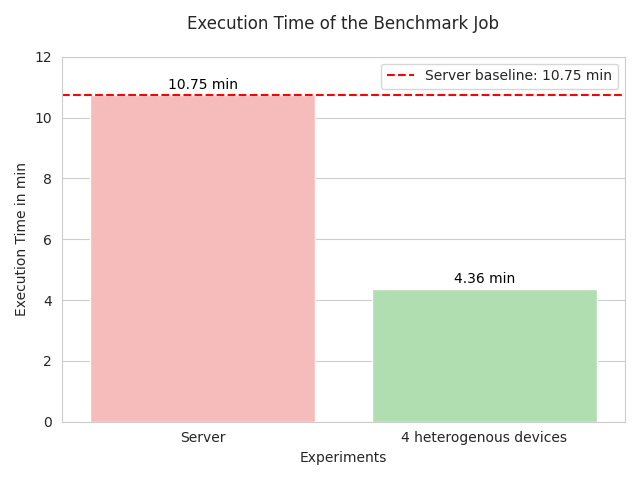
\includegraphics[width=0.95\textwidth]{gfx/figures/Evaluation_C.png}
    \caption{WebCrowd Execution Time with Heterogeneous Set of Workers}
    \label{fig:evaluation:experiment-C}
\end{figure}
~\\
Using the setup of this experiment, the benchmark job was already completed after 4 minutes and 21.6 seconds. This represents a performance improvement of 59\% compared to the native execution on the server. The substantial reduction in execution time demonstrates the effectiveness of WebCrowd's approach to volunteer computing, even when considering the additional overhead of network communication, task scheduling and computation time $t_{Virtual}$ in a WebAssembly environment. This validates that WebCrowd can effectively utilize an environment of heterogeneous devices to achieve significant performance improvements compared to native code execution on a  single system.
\\~\\
The implemented web interface of the client page adapted appropriately to all different screen sizes and resolutions, providing a consistent user experience across all devices. Additionally, the WebWorker implementation effectively prevented any freezing effects of the browser \ac{UI} during the computation of tasks for all participating workers. Therfore, the web application maintained responsiv throughout the experiment and provided real-time monitoring of each worker, as intended.
\\~\\
These results validate that WebCrowd successfully leveraged WebAssembly's platform independence to enable consistent computation across different architectures, while the web-based approach provided a uniform and easy-to-use application, accessible on any device with a modern browser. This confirms that WebCrowd achieves its intended design goal.

\section{Comparison of Implemented WebAssembly Environments}
\label{sec:evaluation:languages}
As WebCrowd currently supports three different programming languages as source for jobs, this section compares the performance of these implemented WebAssembly environments. Each of these programming langues utilizes a unique compilation toolchain to generate the executable WebAssembly binary files and unique JavaScript glue code to handel the corresponding WebAssembly binary in a browser environment, as described in \autoref{sec:methodology:wasm}. A comparison of these implementations can provide valuable insights for potential administrators, which develop new jobs served by a hostet WebCrowd platform.

\subsection{Prime Numbers}
The three implemented WebAssembly environments were evaluated with three other benchmark jobs, each implemented in either C++, Go or Python. Each of these benchmark jobs finds and lists all prime numbers in the range from $0$ to $10.000.000$ and is divided in 10 distinct tasks, each processing a unique intervall of 1 million numbers. All of these 3 prime number jobs have been executed through the WebCrowd platform by a single worker instance, executed in a Apple Safari 18.1 \cite{evaluation:safari} browser on the smartphone specified in \autoref{app:system:phone}.

\autoref{fig:evaluation:experiment-D} compares the total execution time of each prime number job executed in this experiment, revealing significant variations in performance across the different environments. The C++ WebAssembly environment, leveraging the toolchain of emscripten \cite{methodology:emcc}, demonstrated the best computational performance and successfully completed all 10 tasks in only 5.9 seconds. The Go WebAssembly environment, compiled and initialized with the tools provided by Go \cite{methodology:go}, achieved similar but slower execution time of 7.2 seconds for the prime number job. In contrast to these results, the Python WebAssembly environment, utilizing the Pyodide library \cite{methodology:pyodie}, took a total of 156.6 seconds to compute the same workload.
\begin{figure}[htbp]
    \centering
    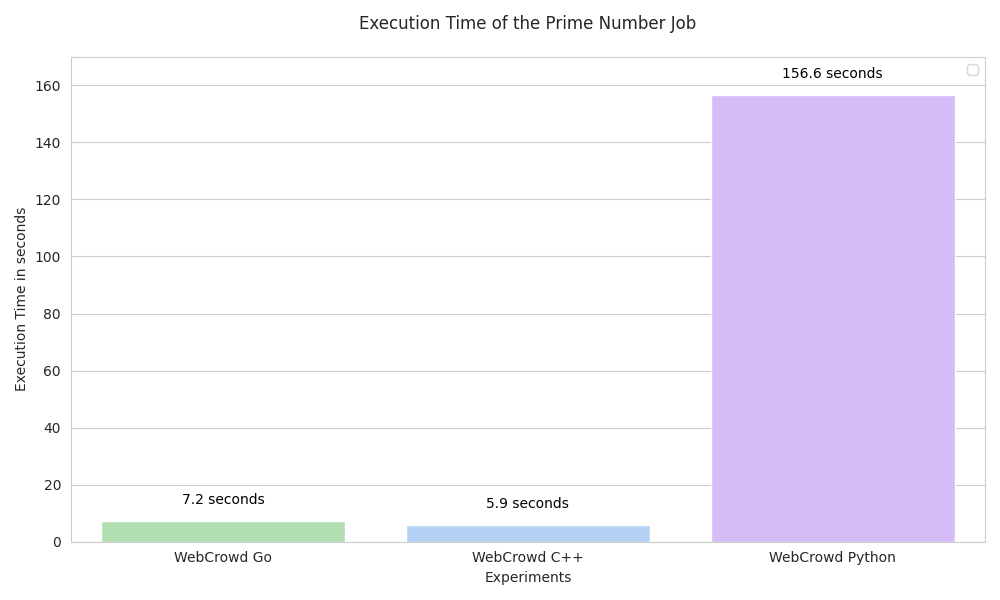
\includegraphics[width=0.95\textwidth]{gfx/figures/Evaluation_D.png}
    \caption{WebCrowd Execution Time of Different WebAssembly Environments}
    \label{fig:evaluation:experiment-D}
\end{figure}
~\\
Despite the fact that all three jobs executed the same workload with a WebAssembly binary on the same system and in the same browser, the execution time of each job varied significantly. The emscripten \cite{methodology:emcc} WebAssembly toolchain demonstrated the best computational performance in this scenerio, however it has not been further investigated why this is the case.

\subsection{Mandelbrot Set}
Additionally to the previous experiment, the implemented C++ and Go WebAssembly environments are further compared in this section. Both environments demonstrated a similar performance when computing the simple prime number job. However, the following experiments again utilize the visualization of Mandelbrot set. The Go source code, compiled with Go \cite{methodology:go} to WebAssembly, can be found in \autoref{app:code:mandelbrot2}, and the according C++ source code, compiled by the emscripten \cite{methodology:emcc} toolchain, can be found in (TODO).

To compare both environment, 
\chapter{Conclusion}
\label{ch:conclusion}
This work has introduced WebArgo, a volunteer computing platform that leverages several modern web technologies to create a new, dynamic and heterogeneous distributed computing solution. Through empirical evaluation, the implemented WebArgo platform has demonstrated its capability to effectively distribute computational workloads across heterogeneous client devices as workers while maintaining robustness in dynamic environments with fluctuating worker participation. 

All three research questions, listed in \autoref{subsec:into:objectives:questions}, were addressed in \autoref{ch:evaluation} and confirmed by the empirical evidence of the evaluations experiments. Furthermore, the experiments revealed that WebArgo is able to successfully reduce the total computation time of the Mandelbrot benchmark job, decribed in \autoref{sec:implementation:benchmark}, by 59\% compared to a native code execution, when distributing the corresponding tasks across four consumer devices found in a single household.

Additionally, WebArgo is successfully fulfilling all its objectives outlined in \autoref{sec:intro:objectives}. Hence, WebArgo provides an accessible volunteer computing solution that requires no setup except a browser and a internet connection for participants.  WebArgo also limits the overhead for administrators, because the development of new jobs does not require a deep understanding of the underlying architecture, and these jobs can be implemented in three different programming languages, through which C/C++ in combination with the emscripten \cite{methodology:emcc} toolchain has turned out to be the currently best performing option. Additionally, hosting a WebArgo instance has limited requirements and can potentially even be used by a single private individual. A public web server with enough storage for the incoming job results and capable of running Docker Compose \cite{conclusion:docker} to orchestrate the backend application, frontend application and database are enough to host a private WebArgo platform.

Furthermore, the web-based approach potentially addressed privacy and security concerns of participants, because installation and execution of third party applications is not required.
\\~\\
In conclusion, WebArgo successfully addresses key challenges in distributed computing while providing an accessible solution for organizations with limited access to traditional \ac{HPC} computing resources. Also its web-based approach reduces any barriers for participation while additionally maintaining the web security model and WebAssembly sandboxing, potentially enabling broader adoption of volunteer computing.


\section{Limitations}
\label{sec:conclusion:limitations}
While WebArgo demonstrates promising capabilities as a volunteer computing platform, several limitations have been identified during its development and evaluation that warrant acknowledgment. The current implementation of the scheduling algorithm operates on a simple \ac{FIFO} basis, without consideration of individual worker hardware capabilities. This approach potentially leads to suboptimal task distribution, as computationally intensive tasks may be assigned to less capable devices while more powerful workers remain underutilized. A more sophisticated scheduling mechanism that accounts for worker hardware specifications and historical performance metrics could improve overall system efficiency.

A significant performance limitation is rooted in the performance of WebAssembly. Despite WebAssembly is promised to perform at near native speed \citeauthor{background:not-so-fast} have discovered, that the WebAssembly execution time can potentially be twice as slow as the corresponding native code execution \cite{background:not-so-fast}, wich is consistent with measurements of this worker. This performance gap impacts WebArgo's computational efficiency. While the parallel processing capabilities of multiple distributed workers can compensate for this limitation, the inherent overhead remains a constraint on individual task performance.

Furthermore, the current implementation is not providing a real multi-threading option for task computation on a single worker device. This limitation prevents full utilization of available computational resources, as workers cannot leverage their potential multi-core capabilities. However, a worker with enough computational capabilitys can effectively execute multiple worker instances to process multiple tasks concurrently, each in an independent browser tap, as experiments of this work confirmed.

Currently, WebArgo's operational scope is constrained to support only one active job at a time. This restriction prevents workers to actively choose wich project or contributor they support with their participation, and therfore potentially reducing volunteer engagement.
\\~\\
These limitations are significant, but do not fundamentally undermine WebArgo's utility as a volunteer computing platform. In fact, these limitations represent opportunities for future development and enhancement of WebArgo.

\section{Future Work}
\label{sec:conclusion:future_work}
This section lists various drafts for future work options. The previously identified limitations of WebArgo provide a clear roadmap for future development and enhancement of the platform.  
\\~\\
\textbf{Performance-Aware Task Scheduling}
\newline
A potential focus for future development is the implementation of an intelligent scheduling algorithm that considers the hardware capabilities of participating workers and assumes the complexity of each task. Therfore, WebArgo could optimize the task distribution across the heterogeneous workers to ensure a optimal utilization of each individual worker.
\\~\\
\textbf{Multi-Threading Support}
\newline
Implementing a approach to enable multi-threaded task execution for workers represents a significant opportunity to further improve the performance WebArgo. This can be achieved either at the source code level by leveraging emscripten's Pthreads support \cite{methodology:emcc} for example, or at the browser level through the initialization of more than one WebWorker instances wich simultaneous process multiple tasks. This additon to WebArgo could be combined with the previously described performance-aware scheduling, hence scheduling multiple tasks for parallel processing to workers with sufficient harware capabilities.
\\~\\
\textbf{Multi-Job Support}
Expanding WebArgo to support multiple actively running jobs simultaneously can improve the user experience for workers. To achieve this, the server needs to handle multiple batches of active tasks and the implemented communication protocol between server and worker needs to be updated. Furthermore, an additional feature to select preferred jobs can be included in the \ac{UI} of the client web page.  
\\~\\
\textbf{Extended Programming Language Support}
While WebArgo currently supports C++, Go, and Python, future work could focus on expanding WebAssembly compilation support for additional programming languages, since WebAssembly is a a compilation target for many more high-level programming languages \cite{methodology:wasm, methodology:wasmW3C, methodology:wasm2}. This can potentially make the platform more accessible to a broader range of developers and scientific computing applications.
\\~\\
\textbf{Implement the MapReduce model}
Implementing the MapReduce \cite{conclusion:map-reduce} model in WebArgo is a big opportunity to significantly enhance the platforms capability of providing more complex jobs. Currently the processing module of a job can be assumed to be similar to the mapping step. Each task therfore represents a single map operation. MapReduce could be used to aggregate all gathered task results of a job to a total result of the job. This enables the processing of more complex jobs like a single epoch of reinforcement learning, with each task representing an episode and the reduce step performing the corresponding policy updates. This approach can be further investigated to potentially enable reinforcement learning through a pipeline of multiple MapReduce jobs in WebArgo.
%*************************************************************************
% Recommendations
%*************************************************************************
%\part{Empfehlungen zur Erstellung wissenschaftlicher Abschlussarbeiten}
%\label{pt:recommendations}
%*************************************************************************
% Backmatter
%*************************************************************************
\appendix
%\renewcommand{\thechapter}{\alph{chapter}}
\cleardoublepage
\part{Appendix}
\chapter{Appendix}
\label{ch:appendix}

\section{System Specifications}
Experiments and code executions have been made on a systems with the following specifications:

\subsection{Local Linux System}
\label{app:system:mymachine}
\begin{itemize}
    \item \textbf{CPU:} Intel(R) Core(TM) i5-8250U CPU @ 1.60GHz
    \item \textbf{RAM:} 15 Gi (15.4667 GB)
    \item \textbf{Operating System:} Ubuntu 20.04.6 LTS
    \item \textbf{Kernel:} 5.15.0-119-generic
    \item \textbf{GPU:} Intel Corporation UHD Graphics 620 (rev 07)
\end{itemize}

\subsection{Local Windows System}
\label{app:system:mypc}
\begin{itemize}
    \item \textbf{CPU:} Intel(R) Core(TM) i7-4790 CPU @ 3.60GHz
    \item \textbf{RAM:} 32 GB
    \item \textbf{Operating System:} Microsoft Windows 10 Home
    \item \textbf{Kernel:} Windows 10.0.19045.5131
    \item \textbf{GPU:} NVIDIA GeForce GTX 1080
\end{itemize}

\subsection{Server Linux System}
\label{app:system:server}
\begin{itemize}
    \item \textbf{CPU:} Intel Xeon Processor (Cascadelake)
    \item \textbf{RAM:} 3.8 Gi
    \item \textbf{Operating System:} Ubuntu 24.04.1 LTS
    \item \textbf{Kernel:} 6.8.0-36-generic
    \item \textbf{GPU:} Cirrus Logic GD 5446
\end{itemize}

\subsection{Raspberry Pi Linux System}
\label{app:system:pi}
\begin{itemize}
    \item \textbf{CPU:} Raspberry Pi 4 Model B Rev 1.4
    \item \textbf{RAM:} 7.7 Gi
    \item \textbf{Operating System:} Ubuntu 22.04.3 LTS
    \item \textbf{Kernel:} 5.15.0-1034-raspi
\end{itemize}

\subsection{Smartphone | iPhone 13}
\label{app:system:phone}
\begin{itemize}
    \item \textbf{Operating System:} iOS 18.1.1
    \item \textbf{CPU:} A15 Bionic chip
    \begin{itemize}
        \item 6-core CPU with 2 performance and 4 efficiency cores \cite{appendix:smartphone}
        \item 4-core GPU \cite{appendix:smartphone}
        \item 16-core Neural Engine \cite{appendix:smartphone}
    \end{itemize}
    \item \textbf{ROM:} 256 GB
\end{itemize}

\subsection{Tablet | iPad Pro 11-inch (3rd generation)}
\label{app:system:tablet}
\begin{itemize}
    \item \textbf{Operating System:} iOS 18.1.1
    \item \textbf{CPU:} Apple M1 chip
    \begin{itemize}
        \item 8-core CPU with 4 performance and 4 efficiency cores \cite{appendix:tablet}
        \item 8-core GPU \cite{appendix:tablet}
        \item 16-core Neural Engine \cite{appendix:tablet}
    \end{itemize}
    \item \textbf{RAM:} 8 GB \cite{appendix:tablet}
    \item \textbf{ROM:} 128 GB
\end{itemize}

\section{Sourcecode and Output}

\subsection{Calculation of Mandelbrot Set: Go}
\label{app:code:mandelbrot1}
Below is the Go source code for generating a colored PNG file of the Mandelbrot set:

\begin{lstlisting}[language=go, frame=tb, caption={Mandelbrot Set Calculation}]
    package main

    import (
        "os"
        "fmt"
        "image"
        "image/color"
        "image/png"
        "math"
        "math/cmplx"
        "time"
    )
    
    func main() {
        startTime := time.Now()
    
        // Set Parameters
        width := 1500
        height := 1500
        maxIterations := 3000
        realMin := -2.0
        realMax := 1.0
        imagMin := -1.5
        imagMax := 1.5
    
        img := image.NewRGBA(image.Rect(0, 0, width, height))
        fmt.Println("Generating PNG of Mandelbrot set... ")
    
        // Calculate Mandelbrot for each Pixel
        for py := 0; py < height; py++ {
            y := imagMax - float64(py)/float64(height)*(imagMax-imagMin)
            for px := 0; px < width; px++ {
                x := float64(px)/float64(width)*(realMax-realMin) + realMin
                z := complex(x, y)
                c := z
                iteration := mandelbrot(z, c, maxIterations)
    
                // Paint Pixel depending on Iteration count
                if iteration >= maxIterations {
                    img.Set(px, py, color.Black)
                } else {
                    img.Set(px, py, colorize(iteration))
                }
            }
        }
    
        // Save PNG
        f, _ := os.Create("mandelbrot_theory.png")
        png.Encode(f, img)
        f.Close()
    
        // Calculate and Print Computation Time
        elapsedTime := time.Since(startTime)
        fmt.Printf("Mandelbrot PNG generation completed in %v\n", elapsedTime)
    }
    
    // Mandelbrot Algorithm
    func mandelbrot(z, c complex128, maxIterations int) (int, float64) {
        var v complex128
        for i := 0; i < maxIterations; i++ {
            if cmplx.Abs(z) > 2 {
                log_zn := math.Log(real(z)*real(z) + imag(z)*imag(z)) / 2
                nu := math.Log(log_zn / math.Log(2)) / math.Log(2)
                return i, float64(i) + 1 - nu
            }
            z = z*z + c
            if z == v {
                return maxIterations, 0
            }
            v = z
        }
        return maxIterations, 0
    }
    
    // Set Color for Pixel
    func colorize(t float64) color.Color {
        t = math.Mod(t*0.1, 1.0) // Adjust color cycle frequency
        hue := 6 * t
        saturation := 1.0
        value := 1.0
        if t >= 1.0 {
            hue = 0
            saturation = 0
            value = 0
        }
    
        hi := math.Floor(hue)
        f := hue - hi
        p := value * (1 - saturation)
        q := value * (1 - saturation*f)
        t = value * (1 - saturation*(1-f))
    
        var r, g, b float64
        switch int(hi) % 6 {
            case 0:
                r, g, b = value, t, p
            case 1:
                r, g, b = q, value, p
            case 2:
                r, g, b = p, value, t
            case 3:
                r, g, b = p, q, value
            case 4:
                r, g, b = t, p, value
            case 5:
                r, g, b = value, p, q
        }
    
        return color.RGBA{
            uint8(r * 255),
            uint8(g * 255),
            uint8(b * 255),
            255,
        }
    }    
\end{lstlisting}

This code has been executed in three isolated runs as follows:
\begin{lstlisting}
    go run mandelbrot_native.go
\end{lstlisting}

The output of this code on the system specified in \ref{app:system:mymachine} was:
\begin{lstlisting}
    Generating PNG of Mandelbrot set... 
    Mandelbrot PNG generation completed in 33.592224199s
\end{lstlisting}
\begin{lstlisting}
    Generating PNG of Mandelbrot set... 
    Mandelbrot PNG generation completed in 34.73396341s
\end{lstlisting}
\begin{lstlisting}
    Generating PNG of Mandelbrot set... 
    Mandelbrot PNG generation completed in 36.602893897s
\end{lstlisting}

\subsection{Calculation of Mandelbrot Set: Go (WASM build)}
\label{app:code:mandelbrot2}
Below is the Go source code for generating a colored PNG file of the Mandelbrot set with all required additions to be compiled to a WebAssembly binary file and executed in the browser:

\begin{lstlisting}[language=go, frame=tb, caption={Mandelbrot Set Calculation (WASM build)}]
    package main

    import (
        "bytes"
        "strconv"
        "fmt"
        "image"
        "image/color"
        "image/png"
        "math"
        "math/cmplx"
        "syscall/js"
        "time"
    )
    
    func main() {
        fmt.Println("Hello WebAssembly")
        c := make(chan bool)
        js.Global().Set("wasmMain", js.FuncOf(wasmMain))
        <-c
    }
    
    func wasmMain(this js.Value, args []js.Value) any {
        startTime := time.Now()
    
        // Get Input Arguments
        width, _ := strconv.Atoi(args[0].String())
        height, _ := strconv.Atoi(args[1].String())
        maxIterations, _ := strconv.Atoi(args[2].String())
        realMin, _ := strconv.ParseFloat(args[3].String(), 64)
        realMax, _ := strconv.ParseFloat(args[4].String(), 64)
        imagMin, _ := strconv.ParseFloat(args[5].String(), 64)
        imagMax, _ := strconv.ParseFloat(args[6].String(), 64)
    
        img := image.NewRGBA(image.Rect(0, 0, width, height))
        fmt.Println("Generating PNG of Mandelbrot set... ")
    
        // Calculate Mandelbrot for each Pixel
        for py := 0; py < height; py++ {
            y := imagMax - float64(py)/float64(height)*(imagMax-imagMin)
            for px := 0; px < width; px++ {
                x := float64(px)/float64(width)*(realMax-realMin) + realMin
                z := complex(x, y)
                c := z
    
                iteration := mandelbrot(z, c, maxIterations)
    
                // Paint Pixel depending on Iteration count
                if iteration >= maxIterations {
                    img.Set(px, py, color.Black)
                } else {
                    img.Set(px, py, colorize(iteration))
                }
            }
        }
    
        // Generate PNG BLOB
        var buf bytes.Buffer
        png.Encode(&buf, img)
    
        elapsedTime := time.Since(startTime)
        fmt.Printf("Mandelbrot PNG generation completed in %v\n", elapsedTime)
    
        // Convert []byte to JS Uint8Array
        uint8Array := js.Global().Get("Uint8Array").New(buf.Len())
        js.CopyBytesToJS(uint8Array, buf.Bytes())
    
        return uint8Array
    }
    
    // Mandelbrot Algorithm
    func mandelbrot(z, c complex128, maxIterations int) (int, float64) {
        var v complex128
        for i := 0; i < maxIterations; i++ {
            if cmplx.Abs(z) > 2 {
                log_zn := math.Log(real(z)*real(z) + imag(z)*imag(z)) / 2
                nu := math.Log(log_zn / math.Log(2)) / math.Log(2)
                return i, float64(i) + 1 - nu
            }
            z = z*z + c
            if z == v {
                return maxIterations, 0
        }
        v = z
        }
        return maxIterations, 0
    }
    
    // Set Color for Pixel
    func colorize(t float64) color.Color {
        t = math.Mod(t*0.1, 1.0) // Adjust color cycle frequency
        hue := 6 * t
        saturation := 1.0
        value := 1.0
        if t >= 1.0 {
            hue = 0
            saturation = 0
            value = 0
        }
    
        hi := math.Floor(hue)
        f := hue - hi
        p := value * (1 - saturation)
        q := value * (1 - saturation*f)
        t = value * (1 - saturation*(1-f))
    
        var r, g, b float64
        switch int(hi) % 6 {
            case 0:
                r, g, b = value, t, p
            case 1:
                r, g, b = q, value, p
            case 2:
                r, g, b = p, value, t
            case 3:
                r, g, b = p, q, value
            case 4:
                r, g, b = t, p, value
            case 5:
                r, g, b = value, p, q
        }
    
        return color.RGBA{
            uint8(r * 255),
            uint8(g * 255),
            uint8(b * 255),
            255,
        }
    }    
\end{lstlisting}

This code was compiled to a WebAssembly binary using the Go \cite{methodology:go} compiler as follows:
\begin{lstlisting}
    GOOS=js GOARCH=wasm go build -o mandelbrot.wasm mandelbrot.go
\end{lstlisting}

\begin{lstlisting}[language=html, frame=tb, caption={Execute \emph{mandelbrot.wasm} in Browser (HTML)}]
    <!DOCTYPE html>
    <html lang="en">
    <head>
        <meta charset="UTF-8">
        <title>Mandelbrot Set with WebAssembly</title>
        <script src="wasm_exec.js"></script>
    </head>
    <body>
        <h1>Mandelbrot Set Calculator</h1>
        <button id="calculate">Calculate Mandelbrot Set</button>
        <br><br>
        <img id="mandelbrotImage" alt="Mandelbrot Set">
        <script>                 
            // Set Up WebAssembly Environment
            const go = new Go();
            let wasmInstance;
    
            WebAssembly.instantiateStreaming(fetch("mandelbrot.wasm"), go.importObject).then((result) => {
                wasmInstance = result.instance;
                go.run(wasmInstance);
            });
    
            document.getElementById('calculate').addEventListener('click', () => {
                const pngData = wasmMain('1500', '1500', '3000', '-2.0', '1.0', '-1.5', '1.5');
                
                // Create a Blob from the PNG data
                const blob = new Blob([pngData], {type: 'image/png'});
                const url = URL.createObjectURL(blob);
                              
                // Display the image
                const img = document.getElementById('mandelbrotImage');
                img.src = url;
                img.onload = () => URL.revokeObjectURL(url);  // Clean up the object URL
            });
        </script>
    </body>
    </html>
\end{lstlisting}

This code has been executed in three isolated runs by accessing the web application with a Mozilla Firefox 132.0 \cite{background:firefox} browser on the system specified in \ref{app:system:mymachine}. The resulting output was:
\begin{lstlisting}
    Generating PNG of Mandelbrot set... 
    Mandelbrot PNG generation completed in 1m11.048999936s
\end{lstlisting}
\begin{lstlisting}
    Generating PNG of Mandelbrot set... 
    Mandelbrot PNG generation completed in 1m11.327000064s
\end{lstlisting}
\begin{lstlisting}
    Generating PNG of Mandelbrot set... 
    Mandelbrot PNG generation completed in 1m11.123000064s
\end{lstlisting}

\subsection{Calculation of Mandelbrot Set: Go (native benchmark)}
\label{app:code:mandelbrot3}
Below is the Go source code for generating 101 unique colored \acs{PNG} files of the Mandelbrot set:

\begin{lstlisting}[language=go, frame=tb, caption={Mandelbrot Set Calculation}]
    package main

    import (
        "os"
        "fmt"
        "image"
        "image/color"
        "image/png"
        "math"
        "math/cmplx"
        "time"
    )

    func main() {
        startTime := time.Now()

        // Set Parameters
        width := 1500
        height := 1500
        maxIterations := 3000
        realMin := -2.0
        realMax := 1.0
        imagMin := -1.5
        imagMax := 1.5
        gridSize := 10
        counter := 0
        realStep := (realMax - realMin) / float64(gridSize)
        imagStep := (imagMax - imagMin) / float64(gridSize) 

        // Generate Thumbnail
        generatePNG(counter, width, height, maxIterations, realMin, realMax, imagMin, imagMax)
        counter++
        // Generating Grid
        for y := 0; y < gridSize; y++ {
            imagLower := imagMax - (float64(y + 1) * imagStep)
            imagUpper := imagMax - (float64(y) * imagStep)
            for x := 0; x < gridSize; x++ {
                realLower := realMin + (float64(x) * realStep)
                realUpper := realMin + (float64(x + 1) * realStep)
                generatePNG(counter, width, height, maxIterations, realLower, realUpper, imagLower, imagUpper)
                counter++
            }   
        }

        // Calculate and Print Computation Time
        elapsedTime := time.Since(startTime)
        fmt.Printf("Mandelbrot PNG generation completed in %v\n", elapsedTime)
    }

    // Generate Mandelbrot PNG
    func generatePNG(counter, width, height, maxIterations int, realMin, realMax, imagMin, imagMax float64) {
        img := image.NewRGBA(image.Rect(0, 0, width, height))
        fmt.Printf("Generating PNG #%v of Mandelbrot set...\n", counter)

        // Calculate Mandelbrot for each Pixel
        for py := 0; py < height; py++ {
            y := imagMax - float64(py)/float64(height)*(imagMax-imagMin)
            for px := 0; px < width; px++ {
                x := float64(px)/float64(width)*(realMax-realMin) + realMin
                z := complex(x, y)
                c := z
                iteration, smooth := mandelbrot(z, c, maxIterations)

                // Paint Pixel depending on Iteration count
                if iteration >= maxIterations {
                    img.Set(px, py, color.Black)
                } else {
                    img.Set(px, py, colorize(smooth))
                }
            }
        }

        // Save PNG
        f, _ := os.Create(fmt.Sprintf("mandelbrot_%d.png", counter))
        png.Encode(f, img)
        f.Close()
    }

    // Mandelbrot Algorithm
    func mandelbrot(z, c complex128, maxIterations int) (int, float64) {
        var v complex128
        for i := 0; i < maxIterations; i++ {
            if cmplx.Abs(z) > 2 {
                log_zn := math.Log(real(z)*real(z) + imag(z)*imag(z)) / 2
                nu := math.Log(log_zn / math.Log(2)) / math.Log(2)
                return i, float64(i) + 1 - nu
            }
            z = z*z + c
            if z == v {
                return maxIterations, 0
            }
            v = z
        }
        return maxIterations, 0
    }

    // Set Color for Pixel
    func colorize(t float64) color.Color {
        t = math.Mod(t*0.1, 1.0) // Adjust color cycle frequency
        hue := 6 * t
        saturation := 1.0
        value := 1.0
        if t >= 1.0 {
            hue = 0
            saturation = 0
            value = 0
        }

        hi := math.Floor(hue)
        f := hue - hi
        p := value * (1 - saturation)
        q := value * (1 - saturation*f)
        t = value * (1 - saturation*(1-f))

        var r, g, b float64
        switch int(hi) % 6 {
            case 0:
                r, g, b = value, t, p
            case 1:
                r, g, b = q, value, p
            case 2:
                r, g, b = p, value, t
            case 3:
                r, g, b = p, q, value
            case 4:
                r, g, b = t, p, value
            case 5:
                r, g, b = value, p, q
        }

        return color.RGBA{
            uint8(r * 255),
            uint8(g * 255),
            uint8(b * 255),
            255,
        }
    }    
\end{lstlisting}

This code has been executed in three isolated runs as follows:
\begin{lstlisting}
    go run mandelbrot_benchmark.go
\end{lstlisting}

The output of this code on the system specified in \ref{app:system:server} was:
\begin{lstlisting}
    Generating PNG #0 of Mandelbrot set...
       [...]
    Generating PNG #100 of Mandelbrot set...
    Mandelbrot PNG generation completed in 10m43.723762025s
\end{lstlisting}
\begin{lstlisting}
    Generating PNG #0 of Mandelbrot set...
       [...]
    Generating PNG #100 of Mandelbrot set...
    Mandelbrot PNG generation completed in 10m48.318590362s
\end{lstlisting}
\begin{lstlisting}
    Generating PNG #0 of Mandelbrot set...
       [...]
    Generating PNG #100 of Mandelbrot set...
    Mandelbrot PNG generation completed in 10m44.884158311s
\end{lstlisting}

\subsection{Calculation of Mandelbrot Set: C++ (WASM build)}
\label{app:code:mandelbrot4}
Below is the C++ source code for generating a colored PNG file of the Mandelbrot set with all required additions to be compiled to a WebAssembly binary file and executed in the browser:

\begin{lstlisting}[language=go, frame=tb, caption={Mandelbrot Set Calculation (WASM build)}]
    #include <emscripten/bind.h>
    #include <emscripten/val.h>
    #include <complex>
    #include <vector>
    #include <cmath>
    #include <chrono>
    #include <iostream>
    #include "lodepng.h"

    using namespace emscripten;

    // Structure to hold iteration result and smooth coloring value
    struct IterationResult {
        int iterations;
        double smooth_value;
    };

    // Color structure
    struct Color {
        uint8_t r;
        uint8_t g;
        uint8_t b;
        uint8_t a;
    };

    // Mandelbrot calculation function
    IterationResult mandelbrot(std::complex<double> z, std::complex<double> c, int maxIterations) {
        std::complex<double> v(0, 0);

        for (int i = 0; i < maxIterations; i++) {
            if (std::abs(z) > 2.0) {
                double log_zn = std::log(std::norm(z)) / 2.0;
                double nu = std::log(log_zn / std::log(2.0)) / std::log(2.0);
                return {i, static_cast<double>(i) + 1.0 - nu};
            }
            z = z * z + c;
            if (z == v) {
                return {maxIterations, 0.0};
            }
            v = z;
        }
        return {maxIterations, 0.0};
    }

    // Color calculation function
    Color colorize(double t) {
        t = fmod(t * 0.1, 1.0); // Adjust color cycle frequency
        double hue = 6.0 * t;
        double saturation = 1.0;
        double value = 1.0;

        if (t >= 1.0) {
            return {0, 0, 0, 255};
        }

        int hi = static_cast<int>(std::floor(hue));
        double f = hue - hi;
        double p = value * (1.0 - saturation);
        double q = value * (1.0 - saturation * f);
        double tt = value * (1.0 - saturation * (1.0 - f));

        double r = 0, g = 0, b = 0;
        switch (hi % 6) {
            case 0: r = value; g = tt; b = p; break;
            case 1: r = q; g = value; b = p; break;
            case 2: r = p; g = value; b = tt; break;
            case 3: r = p; g = q; b = value; break;
            case 4: r = tt; g = p; b = value; break;
            case 5: r = value; g = p; b = q; break;
        }

        return {
            static_cast<uint8_t>(r * 255),
            static_cast<uint8_t>(g * 255),
            static_cast<uint8_t>(b * 255),
            255
        };
    }

    // Main function to generate Mandelbrot set
    std::vector<unsigned char> generateMandelbrot(int width, int height, int maxIterations,
                                                double realMin, double realMax,
                                                double imagMin, double imagMax) {
        std::vector<unsigned char> imageData(width * height * 4);

        // Calculate Mandelbrot for each pixel
        for (int py = 0; py < height; py++) {
            double y = imagMax - static_cast<double>(py) / height * (imagMax - imagMin);
            for (int px = 0; px < width; px++) {
                double x = static_cast<double>(px) / width * (realMax - realMin) + realMin;
                std::complex<double> z(x, y);
                std::complex<double> c = z;

                auto [iteration, smooth] = mandelbrot(z, c, maxIterations);
                Color color;

                if (iteration >= maxIterations) {
                    color = {0, 0, 0, 255}; // Black
                } else {
                    color = colorize(smooth);
                }

                // Set pixel in RGBA format
                size_t idx = (py * width + px) * 4;
                imageData[idx] = color.r;
                imageData[idx + 1] = color.g;
                imageData[idx + 2] = color.b;
                imageData[idx + 3] = color.a;
            }
        }

        return imageData;
    }

    // WebAssembly exposed function
    val wasmMain(val args) {
        // Input validation
        if (!args.isArray()) {
            std::cerr << "Error: Expected array of arguments" << std::endl;
            return val::null();
        }

        // Get array length using proper method
        int argsLength = args["length"].as<int>();

        if (argsLength < 7) {
            std::cerr << "Error: Not enough arguments" << std::endl;
            return val::null();
        }

        // Extract arguments
        int width = args[0].as<int>();
        int height = args[1].as<int>();
        int maxIterations = args[2].as<int>();
        double realMin = args[3].as<double>();
        double realMax = args[4].as<double>();
        double imagMin = args[5].as<double>();
        double imagMax = args[6].as<double>();

        auto startTime = std::chrono::high_resolution_clock::now();
        std::cout << "Generating PNG of Mandelbrot set..." << std::endl;

        // Generate the Mandelbrot image data
        auto imageData = generateMandelbrot(width, height, maxIterations,
                                        realMin, realMax, imagMin, imagMax);

        // Encode to PNG
        std::vector<unsigned char> pngData;
        unsigned error = lodepng::encode(pngData, imageData, width, height);

        if (error) {
            std::cerr << "PNG encoding error: " << error << std::endl;
            return val::null();
        }

        auto endTime = std::chrono::high_resolution_clock::now();
        auto duration = std::chrono::duration_cast<std::chrono::milliseconds>(endTime - startTime);
        std::cout << "Mandelbrot PNG generation completed in " << duration.count() << "ms" << std::endl;

        // Create JavaScript Uint8Array from the PNG data
        val uint8Array = val::global("Uint8Array").new_(pngData.size());
        uint8Array.call<void>("set", val(typed_memory_view(pngData.size(), pngData.data())));

        return uint8Array;
    }

    EMSCRIPTEN_BINDINGS(module) {
        function("wasmMain", &wasmMain);
    }
\end{lstlisting}

This code was compiled to a WebAssembly binary using the emscripten \cite{methodology:emcc} toolchain with the corresponding \emph{loadpng.cpp} file as follows:
\begin{lstlisting}
    emcc mandelbrot10x10-cpp.cpp lodepng.cpp -o mandelbrot10x10-cpp.js -s WASM=1 -s NO_EXIT_RUNTIME=1 -s "EXPORTED_RUNTIME_METHODS=['ccall', 'cwrap']" -s EXPORTED_FUNCTIONS="['_malloc', '_free']" -O3 -s ALLOW_MEMORY_GROWTH=1 -s EXPORT_NAME='GlueCode' -s MODULARIZE=1 -s ENVIRONMENT=worker --bind
\end{lstlisting}
%*************************************************************************
% Other Stuff in the Back
%*************************************************************************
\cleardoublepage%********************************************************************
% Bibliography
%*******************************************************
% work-around to have small caps also here in the headline
% https://tex.stackexchange.com/questions/188126/wrong-header-in-bibliography-classicthesis
% Thanks to Enrico Gregorio
\defbibheading{bibintoc}[\bibname]{%
  \phantomsection
  \manualmark
  \markboth{\spacedlowsmallcaps{#1}}{\spacedlowsmallcaps{#1}}%
  \addtocontents{toc}{\protect\vspace{\beforebibskip}}%
  \addcontentsline{toc}{chapter}{\tocEntry{#1}}%
  \chapter*{#1}%
}

% allow Linebreaks in urls anywhere
\setcounter{biburlnumpenalty}{100}
\setcounter{biburlucpenalty}{100}
\setcounter{biburllcpenalty}{100}
% enable to long words to break anywhere by increasing the allowed whitespace between words.
\sloppy

\printbibliography[heading=bibintoc]

%*************************************************************************
% Game Over: Restore, Restart, or Quit?
%*************************************************************************
\end{document}
%*************************************************************************